% Options for packages loaded elsewhere
\PassOptionsToPackage{unicode}{hyperref}
\PassOptionsToPackage{hyphens}{url}
%
\documentclass[
  ngerman,
]{book}
\usepackage{lmodern}
\usepackage{amsmath}
\usepackage{ifxetex,ifluatex}
\ifnum 0\ifxetex 1\fi\ifluatex 1\fi=0 % if pdftex
  \usepackage[T1]{fontenc}
  \usepackage[utf8]{inputenc}
  \usepackage{textcomp} % provide euro and other symbols
  \usepackage{amssymb}
\else % if luatex or xetex
  \usepackage{unicode-math}
  \defaultfontfeatures{Scale=MatchLowercase}
  \defaultfontfeatures[\rmfamily]{Ligatures=TeX,Scale=1}
\fi
% Use upquote if available, for straight quotes in verbatim environments
\IfFileExists{upquote.sty}{\usepackage{upquote}}{}
\IfFileExists{microtype.sty}{% use microtype if available
  \usepackage[]{microtype}
  \UseMicrotypeSet[protrusion]{basicmath} % disable protrusion for tt fonts
}{}
\makeatletter
\@ifundefined{KOMAClassName}{% if non-KOMA class
  \IfFileExists{parskip.sty}{%
    \usepackage{parskip}
  }{% else
    \setlength{\parindent}{0pt}
    \setlength{\parskip}{6pt plus 2pt minus 1pt}}
}{% if KOMA class
  \KOMAoptions{parskip=half}}
\makeatother
\usepackage{xcolor}
\IfFileExists{xurl.sty}{\usepackage{xurl}}{} % add URL line breaks if available
\IfFileExists{bookmark.sty}{\usepackage{bookmark}}{\usepackage{hyperref}}
\hypersetup{
  pdftitle={Formeln und Flächen},
  pdflang={de},
  hidelinks,
  pdfcreator={LaTeX via pandoc}}
\urlstyle{same} % disable monospaced font for URLs
\usepackage{longtable,booktabs}
\usepackage{calc} % for calculating minipage widths
% Correct order of tables after \paragraph or \subparagraph
\usepackage{etoolbox}
\makeatletter
\patchcmd\longtable{\par}{\if@noskipsec\mbox{}\fi\par}{}{}
\makeatother
% Allow footnotes in longtable head/foot
\IfFileExists{footnotehyper.sty}{\usepackage{footnotehyper}}{\usepackage{footnote}}
\makesavenoteenv{longtable}
\usepackage{graphicx}
\makeatletter
\def\maxwidth{\ifdim\Gin@nat@width>\linewidth\linewidth\else\Gin@nat@width\fi}
\def\maxheight{\ifdim\Gin@nat@height>\textheight\textheight\else\Gin@nat@height\fi}
\makeatother
% Scale images if necessary, so that they will not overflow the page
% margins by default, and it is still possible to overwrite the defaults
% using explicit options in \includegraphics[width, height, ...]{}
\setkeys{Gin}{width=\maxwidth,height=\maxheight,keepaspectratio}
% Set default figure placement to htbp
\makeatletter
\def\fps@figure{htbp}
\makeatother
\usepackage[normalem]{ulem}
% Avoid problems with \sout in headers with hyperref
\pdfstringdefDisableCommands{\renewcommand{\sout}{}}
\setlength{\emergencystretch}{3em} % prevent overfull lines
\providecommand{\tightlist}{%
  \setlength{\itemsep}{0pt}\setlength{\parskip}{0pt}}
\setcounter{secnumdepth}{5}
\usepackage{amsthm}
\usepackage{float}
\usepackage{rotating, graphicx}
\usepackage{multirow}
\usepackage{tabularx}

% new command for pretty oversets with \sim
\newcommand\simcal[1]{\stackrel{\sim}{\smash{\mathcal{#1}}\rule{0pt}{0.5ex}}}

\newcommand{\comma}{,\,}

\floatplacement{figure}{H}

\PassOptionsToPackage{table}{xcolor}

\usepackage{tcolorbox}

\definecolor{kcblue}{HTML}{D7DDEF}
\definecolor{kcdarkblue}{HTML}{2B4E70}

\makeatletter
\def\thm@space@setup{%
  \thm@preskip=8pt plus 2pt minus 4pt
  \thm@postskip=\thm@preskip
}
\makeatother

% \makeatletter % undo the wrong changes made by mathspec
% \let\RequirePackage\original@RequirePackage
% \let\usepackage\RequirePackage
% \makeatother

\newenvironment{rmdknit}
    {\begin{center}
    \begin{tabular}{|p{0.9\textwidth}|}
    \hline\\
    }
    {
    \\\\\hline
    \end{tabular}
    \end{center}
    }

\newenvironment{rmdnote}
    {\begin{center}
    \begin{tabular}{|p{0.9\textwidth}|}
    \hline\\
    }
    {
    \\\\\hline
    \end{tabular}
    \end{center}
    }

\newtcolorbox[auto counter, number within=section]{keyconcepts}[2][]{%
colback=kcblue,colframe=kcdarkblue,fonttitle=\bfseries, title=Key Concept~#2, after title={\newline #1}, beforeafter skip=15pt}

\ifxetex
  % Load polyglossia as late as possible: uses bidi with RTL langages (e.g. Hebrew, Arabic)
  \usepackage{polyglossia}
  \setmainlanguage[]{german}
\else
  \usepackage[shorthands=off,main=ngerman]{babel}
\fi
\ifluatex
  \usepackage{selnolig}  % disable illegal ligatures
\fi
\usepackage[]{natbib}
\bibliographystyle{apalike}

\title{Formeln und Flächen}
\author{}
\date{\vspace{-2.5em}}

\begin{document}
\maketitle

{
\setcounter{tocdepth}{1}
\tableofcontents
}
\hypertarget{was-ist-das}{%
\chapter*{Was ist das?}\label{was-ist-das}}
\addcontentsline{toc}{chapter}{Was ist das?}

Ein Distanzlernpfad zum Thema \emph{Formeln und Flächen}

Hier geht's zur bisherigen \href{https://gdischinger.github.io/Mathe_8d/03FormelnErstellen/FlächenberechnungErinnerung.html}{Seite}. Dort ist alles unverändert\ldots{}

\hypertarget{aktuelles}{%
\subsection*{Aktuelles}\label{aktuelles}}
\addcontentsline{toc}{subsection}{Aktuelles}

\begin{itemize}
\tightlist
\item
  Stichtag für das Abschlussquiz ist der \textbf{28. Februar}
\end{itemize}

\hypertarget{allgemeines}{%
\subsection*{Allgemeines}\label{allgemeines}}
\addcontentsline{toc}{subsection}{Allgemeines}

Dieser Lernpfad soll dir helfen, das große Thema ``Formeln und Flächen'' nicht zu vergessen. Natürlich darfst du auch das Buch zum Nachlesen und zusätzlichen Üben nutzen. Einige Aufgaben, die hier vorkommen, werden mehr oder weniger aus dem Buch übernommen sein.

Da jede*r von euch über individuelles Vorwissen verfügt, wirst du dich mehr oder weniger lang mit diesen Lernpfad beschäftigen müssen wie andere aus deiner Klasse. Es kann sein, dass du feststellst, dass es gut wäre, alte Inhalte noch einmal aufzufrischen oder zu erarbeiten. Arbeite daran, wenn du gerade ein bisschen Zeit hast. In Mathe macht die Übung den Meister - auch die Meisterin.

\hypertarget{binomische-formeln}{%
\chapter{Binomische Formeln}\label{binomische-formeln}}

Die binomischen Formeln sind Spezialfälle der Multiplikation von zwei Summen. Merkt man sich diese drei Formeln, spart man sich oft zwei Zwischenschritte. Damit ist man schneller und macht (hoffentlich) weniger Fehler.

\textbf{Die 1. binomische Formel}

\[(\color{blue}{a}+\color{red}{b})^2= \color{blue}{a}^2 +2\color{blue}{a}\color{red}{b} + \color{red}{b}^2\]

\textbf{Die 2. binomische Formel}

\[(\color{blue}{a}-\color{red}{b})^2= \color{blue}{a}^2 -2\color{blue}{a}\color{red}{b} + \color{red}{b}^2\]

\textbf{Die 3. binomische Formel}

\[(\color{blue}{a}+\color{red}{b})(\color{blue}{a}-\color{red}{b}) = \color{blue}{a}^2 - \color{red}{b}^2\]

\hypertarget{aufgaben}{%
\section*{Aufgaben}\label{aufgaben}}
\addcontentsline{toc}{section}{Aufgaben}

\hypertarget{aufgabe-1}{%
\subsubsection*{Aufgabe 1}\label{aufgabe-1}}
\addcontentsline{toc}{subsubsection}{Aufgabe 1}

Wende die erste binomische Formel an.

\((18u+9a)^2\)

\leavevmode\hypertarget{toggleText1}{}%
\(324u^2+324au+81a^2\)

\((6+22b)^2\)

\leavevmode\hypertarget{toggleText2}{}%
\(484b^2+264b+36\)

\((13+11d)^2\)

\leavevmode\hypertarget{toggleText3}{}%
\(169+286d+121d^2\)

\((16l+11r)^2\)

\leavevmode\hypertarget{toggleText4}{}%
\(256l^2+352lr+121r^2\)

\((24n+5w)^2\)

\leavevmode\hypertarget{toggleText5}{}%
\(576n^2+240nw+25w^2\)

\((14+16s)^2\)

\leavevmode\hypertarget{toggleText6}{}%
\(196+ 448s+256s^2\)

\((8f+14z)^2\)

\leavevmode\hypertarget{toggleText7}{}%
\(64f^2+224fz+196z^2\)

\((h+13i)^2\)

\leavevmode\hypertarget{toggleText8}{}%
\(h^2+26hi+169i^2\)

\((17n+13r)^2\)

\leavevmode\hypertarget{toggleText9}{}%
\(289n^2+442nr+169r^2\)

\((11b+4p)^2\)

\leavevmode\hypertarget{toggleText10}{}%
\(121b^2+88bp+16p^2\)

\((3+18w)^2\)

\leavevmode\hypertarget{toggleText11}{}%
\(9+108w+324w^2\)

\((20i+24h)^2\)

\leavevmode\hypertarget{toggleText12}{}%
\(400i^2+960hi+576h^2\)

\((20r+8i)^2\)

\leavevmode\hypertarget{toggleText13}{}%
\(400r^2+320ir+64i^2\)

\((c+5d)^2\)

\leavevmode\hypertarget{toggleText14}{}%
\(c^2+10cd+25d^2\)

\((7+19x^2)^2\)

\leavevmode\hypertarget{toggleText15}{}%
\(49+266x^2+361x^4\)

\((22s+9fs)^2\)

\leavevmode\hypertarget{toggleText16}{}%
\(484s^2+396fs^2+81f^2s^2\)

\((22b+2l^2)^2\)

\leavevmode\hypertarget{toggleText17}{}%
\(484b^2+88bl^2+4l^4\)

\((15vw+17a)^2\)

\leavevmode\hypertarget{toggleText18}{}%
\(225v^2w^2+510avw+289a^2\)

\((4le+7el)^2\)

\leavevmode\hypertarget{toggleText19}{}%
\(121e^2l^2\)

\((2t^2+23t)^2\)

\leavevmode\hypertarget{toggleText20}{}%
\(4t^4+92t^3+529t^2\)

\((18h^3+13n)^2\)

\leavevmode\hypertarget{toggleText21}{}%
\(324h^6+468h^3n+169n^2\)

\((13+16m^4)^2\)

\leavevmode\hypertarget{toggleText22}{}%
\(169+416m^4+256m^8\)

\((10l+7lp)^2\)

\leavevmode\hypertarget{toggleText23}{}%
\(100l^2+140l^2p+49l^2p^2\)

\((6p+ {7 \over p})^2\)

\leavevmode\hypertarget{toggleText24}{}%
\(36p^2+ 84 +{49 \over p^2}\)

\hypertarget{aufgabe-2}{%
\subsubsection*{Aufgabe 2}\label{aufgabe-2}}
\addcontentsline{toc}{subsubsection}{Aufgabe 2}

Wende die zweite binomische Formel an.

\((2h-15k)^2\)

\leavevmode\hypertarget{toggleText25}{}%
\(4h^2-60hk+225k^2\)

\((6z-5b)^2\)

\leavevmode\hypertarget{toggleText26}{}%
\(36z^2-60bz+25b^2\)

\((22i-19w)^2\)

\leavevmode\hypertarget{toggleText27}{}%
\(484i^2-836iw+361w^2\)

\(((-18c)+19h)^2\)

\leavevmode\hypertarget{toggleText28}{}%
\(324c^2-684ch+361h^2\)

\(((-15m)+24a)^2\)

\leavevmode\hypertarget{toggleText29}{}%
\(576a^2-720am+225m^2\)

\(((-13u)-7l)^2\)

\leavevmode\hypertarget{toggleText30}{}%
\(169u^2+182lu+49l^2\)

\((14e-c^2)^2\)

\leavevmode\hypertarget{toggleText31}{}%
\(196e^2+28ce+c^4\)

\((-3x+3s)^2\)

\leavevmode\hypertarget{toggleText32}{}%
\(9s^2-18sx+9x^2\)

\((22-25s)^2\)

\leavevmode\hypertarget{toggleText33}{}%
\(484-1100s+625s^2\)

\(((-10s)+13qs)^2\)

\leavevmode\hypertarget{toggleText34}{}%
\(100s^2-260qs^2+169q^2s^2\)

\(((-24w)+8z)^2\)

\leavevmode\hypertarget{toggleText35}{}%
\(576w^2-384wz+64z^2\)

\((21b-24z)^2\)

\leavevmode\hypertarget{toggleText36}{}%
\(441b^2-1008bz+576z^2\)

\((16v^2+6)^2\)

\leavevmode\hypertarget{toggleText37}{}%
\(256v^4+192v^2+36\)

\((7t-6do)^2\)

\leavevmode\hypertarget{toggleText38}{}%
\(49t^2-84dot+36d^2o^2\)

\((e-12r)^2\)

\leavevmode\hypertarget{toggleText39}{}%
\(e^2-24er+144r^2\)

\(((-w)+24b)^2\)

\leavevmode\hypertarget{toggleText40}{}%
\(w^2-48bw+576b^2\)

\((15m-25)^2\)

\leavevmode\hypertarget{toggleText41}{}%
\(225m^2-750m+625\)

\(((-6)-22h)^2\)

\leavevmode\hypertarget{toggleText42}{}%
\(36+264h+484h^2\)

\(((-10j)+2q)^2\)

\leavevmode\hypertarget{toggleText43}{}%
\(100j^2-40jq+4q^2\)

\((19l-12t)^2\)

\leavevmode\hypertarget{toggleText44}{}%
\(361l^2-456lt+144t^2\)

\((12w^2-3h^2)^2\)

\leavevmode\hypertarget{toggleText45}{}%
\(144w^4-72h^2w^2+9h^4\)

\(((-8q)-18c)^2\)

\leavevmode\hypertarget{toggleText46}{}%
\(64q^2+288cq+324c^2\)

\(((-15e)-{1,4 \over e})^2\)

\leavevmode\hypertarget{toggleText47}{}%
\(225e^2+42+{1,96 \over e^2}\)

\((6p- {7 \over p})^2\)

\leavevmode\hypertarget{toggleText48}{}%
\(36p^2- 84 +{49 \over p^2}\)

\hypertarget{aufgabe-3}{%
\subsubsection*{Aufgabe 3}\label{aufgabe-3}}
\addcontentsline{toc}{subsubsection}{Aufgabe 3}

Wende die dritte binomische Formel an.

\((8u+9a)(8u-9a)\)

\leavevmode\hypertarget{toggleText49}{}%
\(64u^2-81a^2\)

\((2a+22b)(2a-22b)\)

\leavevmode\hypertarget{toggleText50}{}%
\(4a^2-484b^2\)

\((13d+11)(13d-11)\)

\leavevmode\hypertarget{toggleText51}{}%
\(169d^2-121\)

\((15k+12r)(15k-12r)\)

\leavevmode\hypertarget{toggleText52}{}%
\(225k^2-144r^2\)

\((24v+7w)(24v-7w)\)

\leavevmode\hypertarget{toggleText53}{}%
\(576v^2-49w^2\)

\((16s+14t)(16s-14t)\)

\leavevmode\hypertarget{toggleText54}{}%
\(256s^2-196t^2\)

\(({1 \over 8}f+{3\over 7}e)({1 \over 8}f-{3\over 7}e)\)

\leavevmode\hypertarget{toggleText55}{}%
\({1 \over 64}f^2-{9 \over 49}e^2\)

\((3h+13i)(3h-13i)\)

\leavevmode\hypertarget{toggleText56}{}%
\(9h^2-169i^2\)

\(({5 \over 6} n + 2g)({5 \over 6} n - 2g)\)

\leavevmode\hypertarget{toggleText57}{}%
\({25 \over 36} n^2 - 4g^2\)

\((11b-4p)(11b+4p)\)

\leavevmode\hypertarget{toggleText58}{}%
\(121b^2-16p^2\)

\((3a+17b)(3a-17b)\)

\leavevmode\hypertarget{toggleText59}{}%
\(9a^2-289b^2\)

\((7g+0,4h)(7g-0,4h)\)

\leavevmode\hypertarget{toggleText60}{}%
\(49g^2-0,16h^2\)

\((20r+8i)(20r-8i)\)

\leavevmode\hypertarget{toggleText61}{}%
\(400r^2-64i^2\)

\(({1 \over 2}+b)({1 \over 2}-b)\)

\leavevmode\hypertarget{toggleText62}{}%
\({1 \over 4}-b^2\)

\((7+19x^2)(7-19x^2)\)

\leavevmode\hypertarget{toggleText63}{}%
\(49-361x^4\)

\((21t+9ft)(21t-9ft)\)

\leavevmode\hypertarget{toggleText64}{}%
\(441t^2-81f^2t^2\)

\((12b+2l^2)(12b-2l^2)\)

\leavevmode\hypertarget{toggleText65}{}%
\(144b^2-4l^4\)

\((13vw+16a)(13vw-16a)\)

\leavevmode\hypertarget{toggleText66}{}%
\(169v^2w^2-256a^2\)

\((42da+7ad)(42da-7ad)\)

\leavevmode\hypertarget{toggleText67}{}%
\(1715a^2d^2\)

\((2t^2+11t)(2t^2-11t)\)

\leavevmode\hypertarget{toggleText68}{}%
\(4t^4-121t^2\)

\((6h^3+13n)(6h^3-13n)\)

\leavevmode\hypertarget{toggleText69}{}%
\(36h^6-169n^2\)

\((5+16m^4)(5-16m^4)\)

\leavevmode\hypertarget{toggleText70}{}%
\(25-256m^8\)

\((10l+7lp)(10l-7lp)\)

\leavevmode\hypertarget{toggleText71}{}%
\(100l^2-49l^2p^2\)

\(({10 \over 11}+{7 \over p})({10 \over 11}-{7 \over p})\)

\leavevmode\hypertarget{toggleText72}{}%
\({100 \over 121} - {49 \over p^2}\)

\hypertarget{aufgabe-4}{%
\subsubsection*{Aufgabe 4}\label{aufgabe-4}}
\addcontentsline{toc}{subsubsection}{Aufgabe 4}

Wende eine passende binomische Formel an.

\((1,8j-23g)^2\)

\leavevmode\hypertarget{toggleText73}{}%
\(3,24j^2-82,8gj+529g^2\)

\((1,8j+23g)(1,8j-23g)\)

\leavevmode\hypertarget{toggleText74}{}%
\(3,24j^2-529g^2\)

\((7u-1,3)^2\)

\leavevmode\hypertarget{toggleText75}{}%
\(49u^2-18,2u+1,69\)

\((2,1i+9q)^2\)

\leavevmode\hypertarget{toggleText76}{}%
\(4,41i^2+37,8iq+81q^2\)

\((2,4n-1,6f)^2\)

\leavevmode\hypertarget{toggleText77}{}%
\(5,76n^2-7,68fn+2,56f^2\)

\((-0,5j+0,5l)^2\)

\leavevmode\hypertarget{toggleText78}{}%
\(0,25j^2-0,5jl+0,25l^2\)

\((10h+1,4z)^2\)

\leavevmode\hypertarget{toggleText79}{}%
\(100h^2+28hz+1,96z^2\)

\((1,2x+6h)^2\)

\leavevmode\hypertarget{toggleText80}{}%
\(1,44x^2+14,4hx+36h^2\)

\((2,2t-1,3u)^2\)

\leavevmode\hypertarget{toggleText81}{}%
\(4,84t^2-5,72tu+1,69u^2\)

\((-0,15+2,4u)^2\)

\leavevmode\hypertarget{toggleText82}{}%
\(0,0225-0,72u+5,76u^2\)

\((0,23t-11g)^2\)

\leavevmode\hypertarget{toggleText83}{}%
\(0,0529t^2-5,06gt+121g^2\)

\((10k+{3 \over 4}w)(10k-{3 \over 4}w)\)

\leavevmode\hypertarget{toggleText84}{}%
\(100k^2-{9 \over 16}w^2\)

\(({18 \over 19}v+{7 \over 19})^2\)

\leavevmode\hypertarget{toggleText85}{}%
\({324\over 361}v^2+{252 \over 361}v+{49 \over 361}\)

\((-{12 \over 7}-{3 \over 5}m)^2\)

\leavevmode\hypertarget{toggleText86}{}%
\({144 \over 49}+{72\over 35}m+{9 \over 25}m^2\)

\((-{1\over 3}n+{21 \over 11}l)^2\)

\leavevmode\hypertarget{toggleText87}{}%
\({1 \over 9}n^2 -{14 \over 11}ln + {441\over 121}l^2\)

\(({10 \over 11} + {1 \over 2}n)^2\)

\leavevmode\hypertarget{toggleText88}{}%
\({100 \over 121}+{10 \over 11}n+{1 \over 4}n^2\)

\((2m-{1\over 22}b)(2m+{1\over 22}b)\)

\leavevmode\hypertarget{toggleText89}{}%
\(4m^2-{1 \over 484}b^2\)

\(({1 \over 6}n-{2 \over 3}g)^2\)

\leavevmode\hypertarget{toggleText90}{}%
\({1 \over 36}n^2 - {2 \over 9}gn + {4 \over 9}g^2\)

\(({1 \over 2} +b)({1 \over 2}-b)\)

\leavevmode\hypertarget{toggleText91}{}%
\({1 \over 4}-b^2\)

\((-{1 \over 7}s-{5 \over 8}g)^2\)

\leavevmode\hypertarget{toggleText92}{}%
\({1 \over 49}s^2 + {5 \over 28}gs + {25 \over 64}g^2\)

\(({4 \over 7}n-{5 \over 9})^2\)

\leavevmode\hypertarget{toggleText93}{}%
\({16 \over 49}n^2-{40 \over 63}n+{25 \over 81}\)

\((-{2 \over 3}a-{3 \over 4}b)(-{2 \over 3}a+{3 \over 4}b)\)

\leavevmode\hypertarget{toggleText94}{}%
\({4 \over 9}a^2-{9 \over 4}b^2\)

\(({8 \over 9}r+{1 \over 5}b)^2\)

\leavevmode\hypertarget{toggleText95}{}%
\({64 \over 81}r^2+{16\over 45}br+{1 \over 25}b^2\)

\((-{2 \over 3}r+{3 \over 4}r)^2\)

\leavevmode\hypertarget{toggleText96}{}%
\({1 \over 144}r^2\)

\hypertarget{aufgabe-5}{%
\subsubsection*{Aufgabe 5}\label{aufgabe-5}}
\addcontentsline{toc}{subsubsection}{Aufgabe 5}

Wende eine passende binomische Formel an, um die Summe als Produkt zu schreiben.

\(4r^2-12rx+9x^2\)

\leavevmode\hypertarget{toggleText97}{}%
\((2r-3x)^2\)

\(121z^2+374uz+289u^2\)

\leavevmode\hypertarget{toggleText98}{}%
\((11z+17u)\)

\(4b^2-36bc+81c^2\)

\leavevmode\hypertarget{toggleText99}{}%
\((2b-9c)^2\)

\(k^2-46gk+529g^2\)

\leavevmode\hypertarget{toggleText100}{}%
\((-k+23g)^2\)

\(324j^2+432j+144\)

\leavevmode\hypertarget{toggleText101}{}%
\((18j+12)^2\)

\(400c^2-1000cg+625g^2\)

\leavevmode\hypertarget{toggleText102}{}%
\((20c-25g)^2\)

\(196a^2+56a+4\)

\leavevmode\hypertarget{toggleText103}{}%
\((14a+2)^2\)

\(2,25r^2+15rs+25s^2\)

\leavevmode\hypertarget{toggleText104}{}%
\((1,5r+5s)^2\)

\(16s^4+11,2s^2w+1,96w^2\)

\leavevmode\hypertarget{toggleText105}{}%
\((4s^2+1,4w)^2\)

\(0,16g^2+8gn+100n^2\)

\leavevmode\hypertarget{toggleText106}{}%
\((0,4g+10n)^2\)

\(0,09y^4-2,4y^2z+16z^2\)

\leavevmode\hypertarget{toggleText107}{}%
\((0,3y^2-4z)^2\)

\(4w^4+8,4w^2f^2+4,41f^4\)

\leavevmode\hypertarget{toggleText108}{}%
\((2w^2+2,1f^2)^2\)

\(0,81d^4-16,2d^2l+81l^2\)

\leavevmode\hypertarget{toggleText109}{}%
\((0,9d^2-9l)^2\)

\(400y^4-92y^2k^2+5,29k^4\)

\leavevmode\hypertarget{toggleText110}{}%
\((20y^2-2,3k^2)^2\)

\({1 \over 4}t^2-{6 \over 7}tx+{36 \over 49}x^2\)

\leavevmode\hypertarget{toggleText111}{}%
\(({1 \over 2}t-{6 \over 7}x)^2\)

\({16 \over 81}g^2-{16 \over 45}ga+{4 \over 25}a^2\)

\leavevmode\hypertarget{toggleText112}{}%
\(({4 \over 9}g-{2 \over 5}a)^2\)

\({1 \over 81}h^2+{4 \over 27}hv+{4 \over 9}v^2\)

\leavevmode\hypertarget{toggleText113}{}%
\(({1 \over 9}h+{2 \over 3}v)^2\)

\({9 \over 16}y^2-{2 \over 3}ys+{16 \over 81}s^2\)

\leavevmode\hypertarget{toggleText114}{}%
\(({3 \over 4}y-{4 \over 9}s)^2\)

\({1 \over 4}i^2-{4 \over 5}in+{16 \over 25}n^2\)

\leavevmode\hypertarget{toggleText115}{}%
\(({1 \over 2}i-{4 \over 5}n)^2\)

\({1 \over 16}r^2-{5 \over 16}ir+{25 \over 64}i^2\)

\leavevmode\hypertarget{toggleText116}{}%
\(({1 \over 4}r-{5 \over 8}i)^2\)

\({49 \over 64}i^2-{35 \over 36}gi+{25 \over 81}g^2\)

\leavevmode\hypertarget{toggleText117}{}%
\(({7 \over 8}i-{5 \over 9}g)^2\)

\({25 \over 49}r^2+{10 \over 9}r+{49 \over 81}\)

\leavevmode\hypertarget{toggleText118}{}%
\(({5 \over 7}r+{7 \over 9})^2\)

\({4 \over 81}g^2-{20 \over 63}gh+{25 \over 49}h^2\)

\leavevmode\hypertarget{toggleText119}{}%
\(({2 \over 9}g-{5 \over 7}h)^2\)

\({1 \over 4}j^2+{5 \over 6}ju+{25 \over 36}u^2\)

\leavevmode\hypertarget{toggleText120}{}%
\(({1 \over 2}j+{5 \over 6}u)^2\)

\hypertarget{aufgabe-6}{%
\subsubsection*{Aufgabe 6}\label{aufgabe-6}}
\addcontentsline{toc}{subsubsection}{Aufgabe 6}

Ergänze die Summe um einen Summanden so, dass du sie mit Hilfe der ersten oder zweiten binomischen Formel in ein Produkt umwandeln kannst. Schreibe die geschickt ergänzte Summe anschließend als Produkt.

\(9+576b^2\)

\leavevmode\hypertarget{toggleText121}{}%
\(9-144b+576b^2=(3-24b)^2\)

\(400k^2+324y^2\)

\leavevmode\hypertarget{toggleText122}{}%
\(400k^2+720ky+324y^2=(20k+18y)^2\)

\(44pt+484t^2\)

\leavevmode\hypertarget{toggleText123}{}%
\(p^2+44pt+484t^2=(p+22t)^2\)

\(225b^2-90bc\)

\leavevmode\hypertarget{toggleText124}{}%
\(225b^2-90bc+9c^2=(15b-3c)^2\)

\(46i+529\)

\leavevmode\hypertarget{toggleText125}{}%
\(i^2+46i+529=(i+23)^2\)

\(16w^2+64l^2\)

\leavevmode\hypertarget{toggleText126}{}%
\(16w^2+64wl+64l^2=(4w+8l)^2\)

\(2,56+5,29d^2\)

\leavevmode\hypertarget{toggleText127}{}%
\(2,56+7,36d+5,29d^2=(1,6+2,3d)^2\)

\(100g^2-36gq\)

\leavevmode\hypertarget{toggleText128}{}%
\(100g^2-36gq+3,24q^2=(10g-1,8q)^2\)

\(5,72fl+1,69f^2\)

\leavevmode\hypertarget{toggleText129}{}%
\(4,84l^2+5,72fl+1,69f^2=(2,2l+1,3f)^2\)

\(-10,4sz+16z^2\)

\leavevmode\hypertarget{toggleText130}{}%
\(1,69s^2-10,4sz+16z^2=(1,3s-4z)^2\)

\(4,41n^2+2,25d^2\)

\leavevmode\hypertarget{toggleText131}{}%
\(4,41n^2-6,3dn+2,25d^2=(2,1n-1,5d)^2\)

\(0,81e^2-10,8be\)

\leavevmode\hypertarget{toggleText132}{}%
\(0,81e^2-10,8be+36b^2=(0,9e-6b)^2\)

\({1 \over 14}tz+{25 \over 196}z^2\)

\leavevmode\hypertarget{toggleText133}{}%
\({1 \over 100}t^2+{1 \over 14}tz+{25 \over 196}z^2=({1 \over 10}t+{5 \over 14}z)^2\)

\({16 \over 81}d^2-{2 \over 9}dq\)

\leavevmode\hypertarget{toggleText134}{}%
\({16 \over 81}d^2-{2 \over 9}dq+{1 \over 16}q^2=({4 \over 9}d-{1 \over 4}q)^2\)

\({49 \over 256}v^2+{7 \over 18}vt\)

\leavevmode\hypertarget{toggleText135}{}%
\({49 \over 256}v^2+{7 \over 18}vt+{16 \over 81}t^2=({7 \over 16}v+{4 \over 9}t)^2\)

\({4 \over 5}w+{1 \over 4}w^2\)

\leavevmode\hypertarget{toggleText136}{}%
\({16 \over 25}+{4 \over 5}w+{1 \over 4}w^2=({4 \over 5}+{1 \over 2}w)^2\)

\({36 \over 169}s^2+{25 \over 64}p^2\)

\leavevmode\hypertarget{toggleText137}{}%
\({36 \over 169}s^2+{15 \over 26}sp+{25 \over 64}p^2=({6 \over 13}s+{5 \over 8}p)^2\)

\({36 \over 121}y^2+{25 \over 49}a^2\)

\leavevmode\hypertarget{toggleText138}{}%
\({36 \over 121}y^2+{60 \over 77}ya+{25 \over 49}a^2=({6 \over 11}y+{5 \over 7}a)^2\)

\hypertarget{dreieck}{%
\chapter{Dreieck}\label{dreieck}}

\begin{verbatim}
#> Warning in if (frame.plot) localBox(...): Bedingung hat Länge > 1 und nur das erste Element wird benutzt
\end{verbatim}

\begin{center}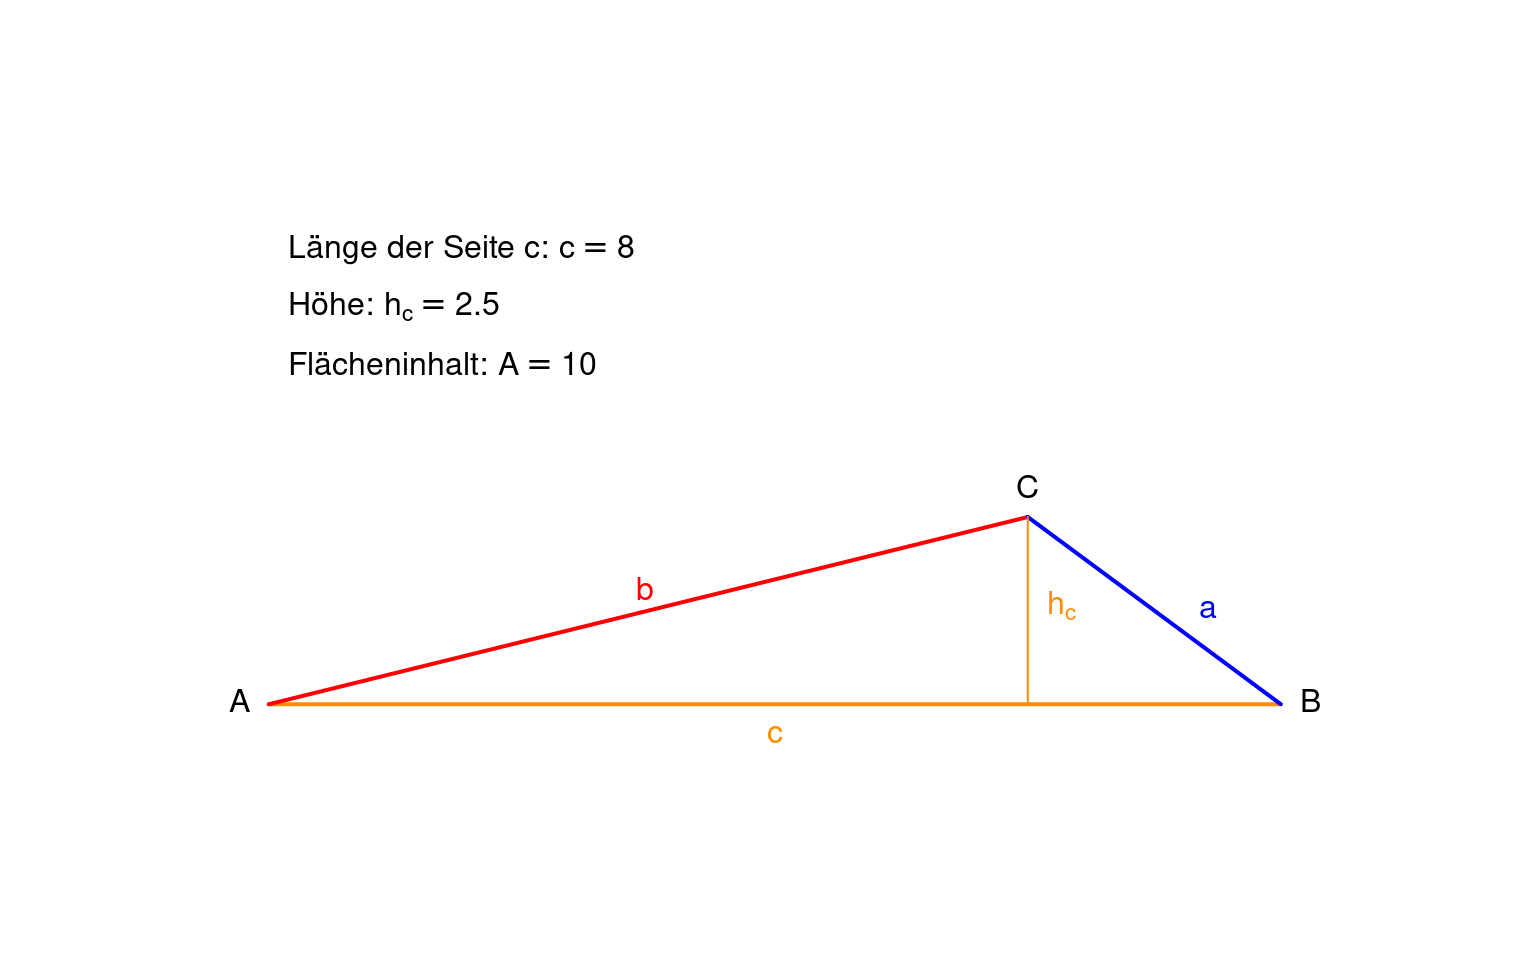
\includegraphics[width=1\linewidth]{Formeln-und-Flächen-8_files/figure-latex/Dreieck-1} \end{center}

\textbf{Flächeninhalt des Dreiecks:}

\[A = {1 \over 2} \cdot g \cdot h\]

\textbf{Umfang des Dreiecks}
\[U = a + b + c\]

\textbf{Was heißt das doch gleich?}

Hier einmal in Worten: Den Flächeninhalt \(A\) eines Dreiecks erhältst du, indem du die Länge der Höhe \(h\) mit der Länge der Grundseite \(g\) multiplizierst und das Ergebnis durch 2 dividierst. Dabei ist es wichtig, dass die Höhe und die Grundseite auch ``zusammengehören''. Im Beispiel oben sind die Grundseite \(c\) und die zugehörige Höhe \(h_c\) eingezeichnet. Die Höhe \(h_c\) gehört zur Grundseite \(c\), weil sie auf dieser senkrecht steht. Sie gehört nicht zur Seite \(a\) und genauso wenig zur Seite \(b\).

Natürlich erhält man denselben Flächeninhalt, wenn man sich für eine andere Grundseite und die dazugehörige Höhe entscheidet. Also:

\[A_{Dreieck} = {1 \over 2} \cdot a \cdot h_{a} = {1 \over 2} \cdot b \cdot h_{b} = {1 \over 2} \cdot c \cdot h_{c}\]

\hypertarget{aufgaben-1}{%
\section*{Aufgaben}\label{aufgaben-1}}
\addcontentsline{toc}{section}{Aufgaben}

\hypertarget{aufgabe-1-1}{%
\subsubsection*{Aufgabe 1}\label{aufgabe-1-1}}
\addcontentsline{toc}{subsubsection}{Aufgabe 1}

Berechne die fehlende Größe des Dreiecks.

\begin{longtable}[]{@{}llll@{}}
\toprule
& a) & b) & c)\tabularnewline
\midrule
\endhead
Grundseite g & 3 cm & & 8cm\tabularnewline
Höhe h & 6 cm & 30 cm &\tabularnewline
Flächeninhalt A & & 24 cm² & 12 cm²\tabularnewline
\bottomrule
\end{longtable}

Lösung

Die fehlende Größe des Dreiecks lautet:

\begin{longtable}[]{@{}llll@{}}
\toprule
& a) & b) & c)\tabularnewline
\midrule
\endhead
Grundseite g & 3 cm & \textbf{1,6cm} & 8cm\tabularnewline
Höhe h & 6 cm & 30 cm & \textbf{3cm}\tabularnewline
Flächeninhalt A & \textbf{9 cm²} & 24 cm² & 12 cm²\tabularnewline
\bottomrule
\end{longtable}

\textbf{Rechnungen:}

\[\begin{align} a) \quad\quad A &= {1 \over 2} \cdot g \cdot h \\
{}\\
A &= {1 \over 2} \cdot 3 cm \cdot 6 cm \\
{}\\
A&= 9 cm² \quad \end{align}\]

\[\begin{align} b) \quad\quad A\quad &= {1 \over 2} \cdot g \cdot h \\
{}\\
24 cm² &= {1 \over 2} \cdot g \cdot 30cm \\
{}\\
24 cm² &= {1 \over 2} \cdot 30cm \cdot g \\
{}\\
24 cm² &= 15cm \cdot g  \quad\quad | : 15 cm\\
{}\\
{8 \over 5} cm &= g\\
{}\\
\Rightarrow g &= 1,6 cm \end{align}\]

\[ \begin{align} c) \quad\quad A\quad &= {1 \over 2} \cdot g \cdot h \\
{}\\
12 cm² &= {1 \over 2} \cdot 8cm \cdot h\\
{}\\
12 cm² &= 4cm \cdot h \quad |:4cm\\
{}\\
3cm &= h \end{align}\]

\hypertarget{section}{%
\subsubsection*{}\label{section}}
\addcontentsline{toc}{subsubsection}{}

\hypertarget{aufgabe-2-1}{%
\subsubsection*{Aufgabe 2}\label{aufgabe-2-1}}
\addcontentsline{toc}{subsubsection}{Aufgabe 2}

Gegeben ist ein Dreieck mit Grundseite \(g\) und Höhe \(h\). Wie verändert sich der Flächeninhalt, wenn die Höhe verdoppelt/vervierfacht/halbiert wird?

\hypertarget{section-1}{%
\paragraph*{}\label{section-1}}
\addcontentsline{toc}{paragraph}{}

Tipp 1

Betrachte zunächst folgende Animation:

\begin{verbatim}
#> Warning in if (frame.plot) localBox(...): Bedingung hat Länge > 1 und nur das erste Element wird benutzt
\end{verbatim}

\begin{center}\animategraphics[width=1\linewidth,controls,loop]{0.769230769230769}{Formeln-und-Flächen-8_files/figure-latex/dirac1-}{1}{11}\end{center}

Notiere deine Beobachtungen:

\begin{itemize}
\item
  Wenn die Höhe verdoppelt wird, \ldots\ldots{} sich der Flächeninhalt.
\item
  Wenn die Höhe vervierfacht wird, \ldots. sich der Flächeninhalt.
\item
  Wenn die Höhe halbiert wird, \ldots{} sich der Flächeninhalt.
\end{itemize}

\hypertarget{section-2}{%
\paragraph*{}\label{section-2}}
\addcontentsline{toc}{paragraph}{}

Tipp 2

Versuche nun deine Beobachtungen auch zu zeigen. Verändere dafür die Variablen in der Gleichung zur Berechnung des Flächeninhaltes eines Dreiecks auf geeignete Weise.

\hypertarget{section-3}{%
\paragraph*{}\label{section-3}}
\addcontentsline{toc}{paragraph}{}

Lösung

\begin{itemize}
\tightlist
\item
  Folgende Beobachtungen lassen sich hier notieren:

  \begin{itemize}
  \tightlist
  \item
    Wenn die Höhe verdoppelt wird, \textbf{verdoppelt} sich der Flächeninhalt.
  \item
    Wenn die Höhe vervierfacht wird, \textbf{vervierfacht} sich der Flächeninhalt.
  \item
    Wenn die Höhe halbiert wird, \textbf{halbiert} sich der Flächeninhalt.
  \end{itemize}
\end{itemize}

Beweis:
Den Flächeninhalt eines Dreiecks berechnet man folgendermaßen:
\[ A = {1 \over 2} \cdot g \cdot h \]
Verdoppelt man die Höhe \(h\), so erhält man eine neue Höhe der Länge \(2h\), für die Berechnung des Flächeninhaltes \(A_{neu}\) des neuen Dreiecks mit der verdoppelten Höhe ergibt sich dann:
\[\begin{align} A_{neu} &= {1 \over 2} \cdot g \cdot (2h) = \\
&= 2 \cdot \underbrace{\left({1 \over 2} \cdot g \cdot h\right)}_{=A} =  2 \cdot A \end{align}\]
Damit ist der neue Flächeninhalt, der zur verdoppelten Höhe gehört, doppelt (zweimal) so groß wie der alte Flächeninhalt.

Die beiden anderen Aussagen zeigt man genauso! Versuch's doch auch mal mit der vierfachen Höhe!

\hypertarget{section-4}{%
\subsubsection*{}\label{section-4}}
\addcontentsline{toc}{subsubsection}{}

\hypertarget{aufgabe-3-1}{%
\subsubsection*{Aufgabe 3}\label{aufgabe-3-1}}
\addcontentsline{toc}{subsubsection}{Aufgabe 3}

In einem Dreieck beträgt der Flächeninhalt \(A=20cm²\). Die Höhe \(h_c\) ist doppelt so lang wie die zugehörige Grundseite \(c\). Berechne \(c\) und \(h_c\).

Lösung

\textbf{Gegeben}

Gegeben ist also:

\begin{enumerate}
\def\labelenumi{\arabic{enumi}.}
\tightlist
\item
  Der Flächeninhalt: \(A=20cm²\) und
\item
  der Hinweis, dass die Höhe \(h_c\) doppelt so lang ist wie die zugehörige Grundseite \(c\), also: \(h_c= 2 \cdot c\).
\end{enumerate}

Den Flächeninhalt eines Dreiecks berechnet man folgendermaßen:
\[ A = {1 \over 2} \cdot c \cdot h_c \]

\textbf{Einsetzen}

Setzt man nun alle Angaben ein, erhält man folgenden Gleichung:

\[ 20 cm² = {1 \over 2} \cdot c \cdot (2c) \]

\textbf{Auflösen}

Diese Gleichung muss man jetzt nach \(c\) auflösen:

\[ \begin{align} 20 cm² &= {1 \over 2} \cdot c \cdot (2c) \\
{}\\
20 cm² &= {1 \over 2} \cdot 2 \cdot c \cdot c \\
{}\\
20 cm² &= c² \quad\quad\quad |\sqrt{\quad}\\
{}\\
\Rightarrow c &= \sqrt{20} cm \approx 4,47 cm \\
\Rightarrow h_c &= 2 \cdot c = 2 \cdot \sqrt{20} cm \approx 8,94cm
\end{align}\]

\textbf{Antwort}

Die Seite \(c\) ist also ungefähr 4,47 cm lang und die Höhe \(h_c\) hat eine Länge von etwa 8,94 cm.

\hypertarget{section-5}{%
\subsubsection*{}\label{section-5}}
\addcontentsline{toc}{subsubsection}{}

\hypertarget{aufgabe-4-1}{%
\subsubsection*{Aufgabe 4}\label{aufgabe-4-1}}
\addcontentsline{toc}{subsubsection}{Aufgabe 4}

Berechne den Flächeninhalt des Dreiecks. Wähle dafür passende Größen aus.

\begin{longtable}[]{@{}llll@{}}
\toprule
\begin{minipage}[b]{(\columnwidth - 3\tabcolsep) * \real{0.26}}\raggedright
\strut
\end{minipage} & \begin{minipage}[b]{(\columnwidth - 3\tabcolsep) * \real{0.26}}\raggedright
a)\strut
\end{minipage} & \begin{minipage}[b]{(\columnwidth - 3\tabcolsep) * \real{0.26}}\raggedright
b)\strut
\end{minipage} & \begin{minipage}[b]{(\columnwidth - 3\tabcolsep) * \real{0.22}}\raggedright
c)\strut
\end{minipage}\tabularnewline
\midrule
\endhead
\begin{minipage}[t]{(\columnwidth - 3\tabcolsep) * \real{0.26}}\raggedright
gegebene Seiten\strut
\end{minipage} & \begin{minipage}[t]{(\columnwidth - 3\tabcolsep) * \real{0.26}}\raggedright
\(a=5cm\), \(b=4cm\)\strut
\end{minipage} & \begin{minipage}[t]{(\columnwidth - 3\tabcolsep) * \real{0.26}}\raggedright
\(b=8m\), \(c=6m\)\strut
\end{minipage} & \begin{minipage}[t]{(\columnwidth - 3\tabcolsep) * \real{0.22}}\raggedright
\(b=4cm\), \(c=5cm\)\strut
\end{minipage}\tabularnewline
\begin{minipage}[t]{(\columnwidth - 3\tabcolsep) * \real{0.26}}\raggedright
gegebene Höhen\strut
\end{minipage} & \begin{minipage}[t]{(\columnwidth - 3\tabcolsep) * \real{0.26}}\raggedright
\(h_a = 2,4 cm\), \(h_b = 3cm\)\strut
\end{minipage} & \begin{minipage}[t]{(\columnwidth - 3\tabcolsep) * \real{0.26}}\raggedright
\(h_b =3,75m\), \(h_c =5m\)\strut
\end{minipage} & \begin{minipage}[t]{(\columnwidth - 3\tabcolsep) * \real{0.22}}\raggedright
\(h_a =2cm\), \(h_b = 3,1 cm\)\strut
\end{minipage}\tabularnewline
\bottomrule
\end{longtable}

Lösung

\textbf{a)}

Für die Berechnung des Flächeninhaltes des Dreiecks wähle ich die Seite \(b=4cm\) und die zugehörige Höhe \(h_b = 3cm\), da die Rechnung mit diesen Angaben ein bisschen einfacher ist.

Rechnung: \[ \begin{align} A &= {1 \over 2} \cdot g \cdot h \\
                            {}\\
                             & = {1 \over 2} \cdot 4 cm \cdot 3cm  \\
                             {}\\
                             & = 6 cm² \end{align}\]

\textbf{b)}

Für die Berechnung des Flächeninhaltes des Dreiecks wähle ich die Seite \(c=6m\) und die zugehörige Höhe \(h_c = 5m\), da die Rechnung mit diesen Angaben ein bisschen einfacher ist.

Rechnung: \[ \begin{align} A &= {1 \over 2} \cdot g \cdot h \\
                              {}\\
                              & = {1 \over 2} \cdot 6m \cdot 5m \\ 
                              {}\\
                              & = 15m² \end{align}\]

\textbf{c)}

Für die Berechnung des Flächeninhaltes des Dreiecks wähle ich die Seite \(b=4cm\) und die zugehörige Höhe \(h_b = 3,1 cm\). Zur Seite \(c\) fehlt die Angabe der zugehörigen Höhe \(h_c\), ebenso wie zur Höhe \(h_a\) die Angabe der zugehörigen Seite \(a\) fehlt.

Rechnung: \[ \begin{align} A & = {1 \over 2} \cdot g \cdot h \\
                              {}\\
                              & = {1 \over 2} \cdot 4cm \cdot 3,1cm \\
                              {}\\
                              & = 6,2 cm²\end{align} \]

\hypertarget{section-6}{%
\subsubsection*{}\label{section-6}}
\addcontentsline{toc}{subsubsection}{}

\hypertarget{aufgabe-5---zusatzaufgabe}{%
\subsubsection*{\texorpdfstring{Aufgabe 5 - \textbf{Zusatzaufgabe}}{Aufgabe 5 - Zusatzaufgabe}}\label{aufgabe-5---zusatzaufgabe}}
\addcontentsline{toc}{subsubsection}{Aufgabe 5 - \textbf{Zusatzaufgabe}}

Im folgenden mathematischen ``Versuchsaufbau'' kannst du mit einem Dreieck experimentieren. Ziehe an den Ecken. Verschiebe sie. Beobachte, wie sich die Höhen verhalten. Wirf auch einen Blick auf die Formeln zur Berechnung des Flächeninhaltes.

\begin{enumerate}
\def\labelenumi{\alph{enumi})}
\item
  Verändere das Dreieck so, dass eine Höhe außerhalb des Dreiecks liegt. Schaffst du es, dass nur eine Höhe außerhalb des Dreiecks liegt?
\item
  Verändere das Dreieck so, dass eine Höhe genau auf einer Dreiecksseite liegt. Schaffst du es, dass nur eine Höhe auf einer Dreiecksseite liegt? Welches besondere Dreieck entsteht, wenn eine Höhe mit einer Dreiecksseite übereinstimmt? Was fällt dir in diesem Fall bei den Formeln zur Berechnung des Flächeninhaltes auf?
\item
  Konstruiere drei unterschiedliche Dreiecke mit dem Flächeninhalt 100.
\end{enumerate}

\hypertarget{aufgabe-6---zusatzaufgabe}{%
\subsubsection*{\texorpdfstring{Aufgabe 6 - \textbf{Zusatzaufgabe}}{Aufgabe 6 - Zusatzaufgabe}}\label{aufgabe-6---zusatzaufgabe}}
\addcontentsline{toc}{subsubsection}{Aufgabe 6 - \textbf{Zusatzaufgabe}}

Berechne die fehlende Größe des Dreiecks.

\begin{longtable}[]{@{}lllllll@{}}
\toprule
& a) & b) & c) & d) & e) & f)\tabularnewline
\midrule
\endhead
Grundseite g & \(6 cm\) & \(4 m\) & & \({1 \over 2}cm\) & \(3,2 km\) &\tabularnewline
Höhe h & & & \(8400 m\) & \(8cm\) & & \(125cm\)\tabularnewline
Flächeninhalt A & \(12,6 cm^2\) & \(32 m^2\) & \(10,08 km^2\) & & \(8,64 km^2\) & \(2 m^2\)\tabularnewline
\bottomrule
\end{longtable}

\hypertarget{aufgabe-7---zusatzaufgabe}{%
\subsubsection*{\texorpdfstring{Aufgabe 7 - \textbf{Zusatzaufgabe}}{Aufgabe 7 - Zusatzaufgabe}}\label{aufgabe-7---zusatzaufgabe}}
\addcontentsline{toc}{subsubsection}{Aufgabe 7 - \textbf{Zusatzaufgabe}}

Zeichne das Dreieck in ein Koordinatensystem und ermittle den Flächeninhalt. Wähle als Achseneinteilung 2 Kästchen = 1 Einheit.

\begin{enumerate}
\def\labelenumi{\alph{enumi})}
\item
  A(3\textbar0); B(8\textbar0); C(6\textbar5)
\item
  A(9\textbar1); B(9\textbar9); C(5\textbar5)
\end{enumerate}

\hypertarget{aufgabe-8---zusatzaufgabe}{%
\subsubsection*{\texorpdfstring{Aufgabe 8 - \textbf{Zusatzaufgabe}}{Aufgabe 8 - Zusatzaufgabe}}\label{aufgabe-8---zusatzaufgabe}}
\addcontentsline{toc}{subsubsection}{Aufgabe 8 - \textbf{Zusatzaufgabe}}

\begin{figure}
\centering
\includegraphics[width=6.25in,height=\textheight]{./Bilder/FlächenberechnungDreieckFehlerFinden.png}
\caption{Erkläre und korrigiere den Fehler.}
\end{figure}

\hypertarget{parallelogramm}{%
\chapter{Parallelogramm}\label{parallelogramm}}

\begin{verbatim}
#> Warning in if (frame.plot) localBox(...): Bedingung hat Länge > 1 und nur das erste Element wird benutzt
\end{verbatim}

\begin{center}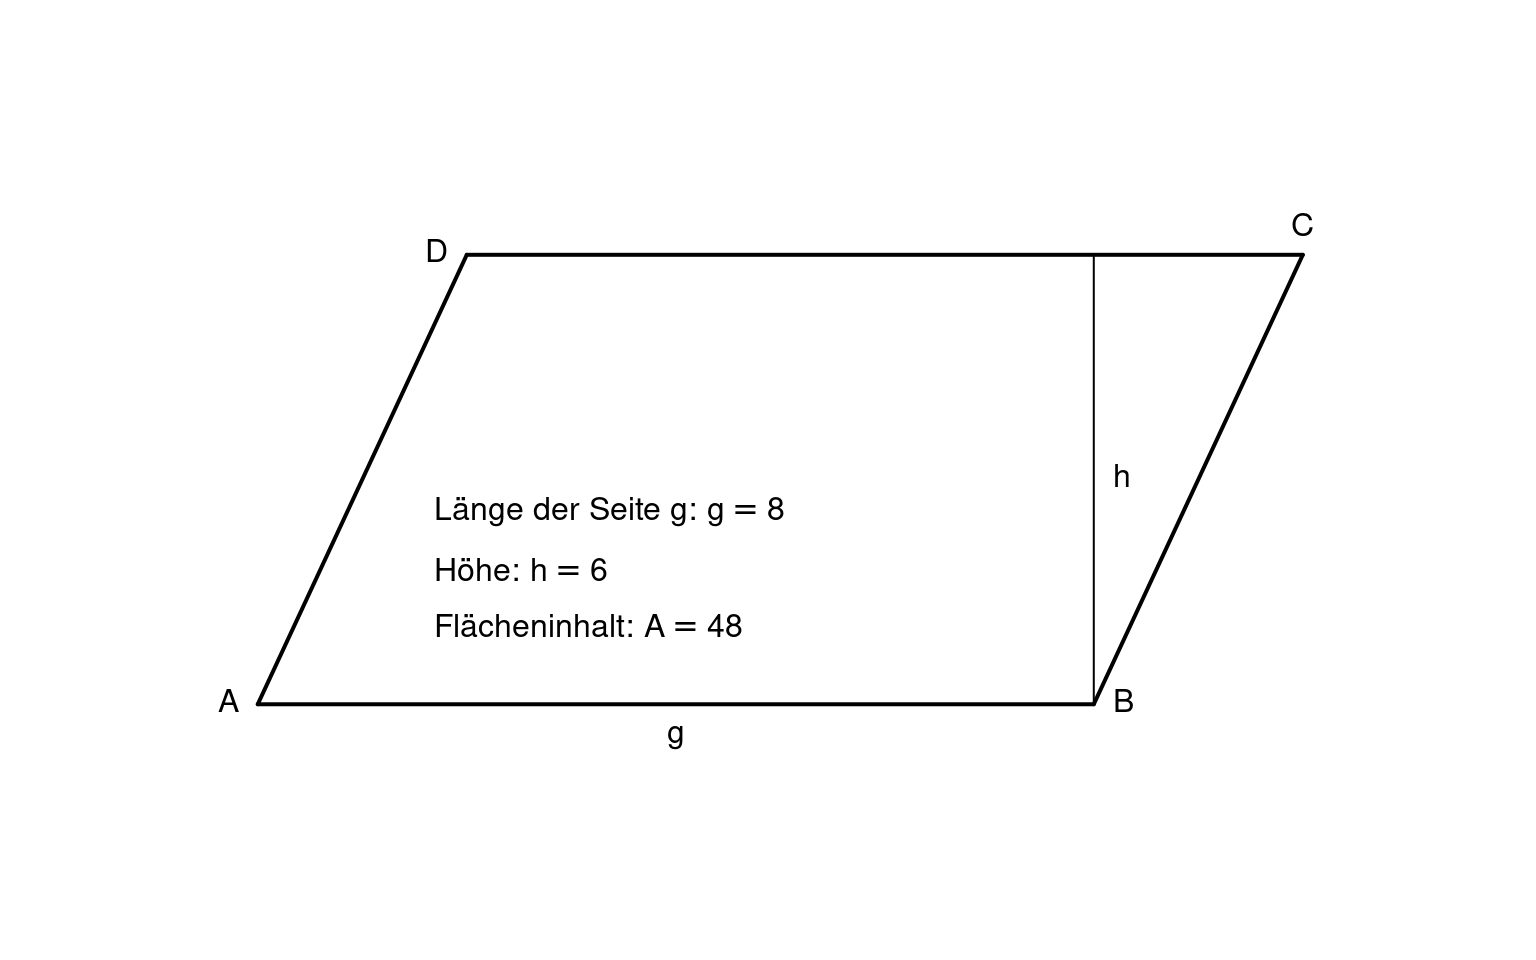
\includegraphics[width=1\linewidth]{Formeln-und-Flächen-8_files/figure-latex/Parallelogramm-1} \end{center}

\textbf{Flächeninhalt des Parallelogramms:}

\[A = g \cdot h\]

\textbf{Umfang des Parallelogramms}
\[U = a + b + c + d\]

\[U = a + b + c\]

\textbf{Was heißt das doch gleich?}

Hier einmal in Worten: Den Flächeninhalt \(A\) eines Parallelogramms erhältst du, indem du die Länge der Höhe \(h\) mit der Länge der Grundseite \(g\) multiplizierst. Dabei ist es wichtig, dass die Höhe und die Grundseite auch ``zusammengehören''. Die Höhe \(h\) im obigen Beispiel gehört zur Grundseite \(g\), weil sie auf dieser senkrecht steht.

\hypertarget{aufgaben-2}{%
\section*{Aufgaben}\label{aufgaben-2}}
\addcontentsline{toc}{section}{Aufgaben}

\hypertarget{aufgabe-1-2}{%
\subsubsection*{Aufgabe 1}\label{aufgabe-1-2}}
\addcontentsline{toc}{subsubsection}{Aufgabe 1}

Berechne die fehlende Größe des Parallelogramms.

\begin{longtable}[]{@{}llll@{}}
\toprule
& a) & b) & c)\tabularnewline
\midrule
\endhead
Grundseite g & 5 cm & & 90 mm\tabularnewline
Höhe h & 3 cm & 25 cm &\tabularnewline
Flächeninhalt A & & 625 cm² & 72 cm²\tabularnewline
\bottomrule
\end{longtable}

Lösung

\textbf{Die fehlende Größe des Parallelogramms lautet:}

\begin{longtable}[]{@{}llll@{}}
\toprule
& a) & b) & c)\tabularnewline
\midrule
\endhead
Grundseite g & 3 cm & \textbf{25cm} & 8cm\tabularnewline
Höhe h & 6 cm & 30 cm & \textbf{8cm}\tabularnewline
Flächeninhalt A & \textbf{15 cm²} & 24 cm² & 12 cm²\tabularnewline
\bottomrule
\end{longtable}

\textbf{Rechnungen:}

\textbf{a)}

\[\begin{align} A &= g \cdot h \\
{}\\
A &= 5 cm \cdot 3 cm \quad\quad\quad \\
{}\\
A &= 15 cm² \end{align}\]

\textbf{b)}

\[\begin{align} A \quad &= g \cdot h \\
{}\\
625 cm² &= g \cdot 25cm  \quad | : 25 cm\quad\quad\quad\\
{}\\
25 cm &= g \end{align}\]

\textbf{c)}

\[ \begin{align} A\quad &=  g \cdot h \\
{}\\
72 cm² &= 90mm \cdot h\\
{}\\
72 cm² &= 9cm \cdot h \quad |:9cm\\
{}\\
8cm &= h \end{align}\]

\hypertarget{section-7}{%
\subsubsection*{}\label{section-7}}
\addcontentsline{toc}{subsubsection}{}

\hypertarget{aufgabe-2-2}{%
\subsubsection*{Aufgabe 2}\label{aufgabe-2-2}}
\addcontentsline{toc}{subsubsection}{Aufgabe 2}

Frau Dischinger behauptet:

\begin{quote}
``Der Flächeninhalt eines Parallelogramms ändert sich nicht, wenn man eine Grundseite halbiert und die zugehörige Höhe verdoppelt.''
\end{quote}

Stimmt das?
Begründe deine Antwort.

Lösung

\textbf{Ja, das stimmt!}

Begründung:

Die Grundseite \(g\) wird halbiert, das heißt, man erhält eine neue Grundseite \(g_{neu}\), die halb so lang ist, wie die alte Grundseite \(g\), also: \(g_{neu}={1 \over 2} \cdot g\).
Gleichzeitig wird die Höhe \(h\) verdoppelt, das heißt man erhält eine neue Höhe \(h_{neu}\), die zweimal so lang ist, wie die alte Höhe \(h\), also \(h_{neu}= 2 \cdot h\).

Damit ergibt sich für den neuen Flächeninhalt:
\[\begin{align} A_{neu} &= g_{neu} \cdot h_{neu} = \\
{}\\
& = {1 \over 2} \cdot g \cdot 2 \cdot h =\\
{}\\
& = {1 \over 2} \cdot 2 \cdot g \cdot h =\\
{}\\
&= g \cdot h = A \end{align}\]

\hypertarget{section-8}{%
\subsubsection*{}\label{section-8}}
\addcontentsline{toc}{subsubsection}{}

\hypertarget{aufgabe-3-2}{%
\subsubsection*{Aufgabe 3}\label{aufgabe-3-2}}
\addcontentsline{toc}{subsubsection}{Aufgabe 3}

Ein Rechteck und ein Parallelogramm haben die gleiche Grundseite. Was weißt du über das Parallelogramm, wenn der Flächeninhalt des Rechtecks doppelt so groß ist wie der des Parallelogramms? Erläutere.

Lösung

Wenn der Flächeninhalt des Rechtecks doppelt so groß ist wie der Flächeninhalt des Parallelogramms (\(A_R = 2 \cdot A_P\)) und die eine Seite des Rechtecks genauso lang ist wie die Grundseite des Parallelogramms (\(l=g\)), dann muss die andere Rechtecksseite doppelt so lang sein wie Höhe des Parallelogramms (\(b=2h\)).

Was natürlich genau das Gleiche ist, wie zu sagen, dass die Höhe des Parallelogramms halb so lang sein muss wie die andere Rechtecksseite (\(h={1 \over 2} \cdot b\)).

\textbf{Erläuterung}

Für den Flächeninhalt eines Rechtecks gilt: \(\quad\quad\quad\quad A_{R}= Länge \cdot Breite = l \cdot b\).

Für den Flächeninhalt eines Parallelogramms gilt: \(\quad\quad A_{P} = Grundseite \cdot Höhe = g \cdot h\)

Aus der Aufgabenstellung ist bekannt:

\[\begin{align} &1. \quad A_{R} = 2 \cdot A_{P} \\
                {}\\
                &2. \quad l = g \end{align}\]

Damit muss \(b= 2 \cdot h\) sein oder, wenn man die Gleichung durch \(2\) dividiert, \(h={1 \over 2} \cdot b\).

Denn:
\[\begin{align} \underbrace{A_R}_{=l \cdot r} &= 2 \cdot A_{P}= 2 \cdot g \cdot h = 2 \cdot l \cdot h = l \cdot (2h)\\
{}\\
\Leftrightarrow \quad l \cdot b &= l \cdot (2h) \quad\quad |:l\\
                  {}\\
                 b &= 2h  \quad\quad |:2 \\
                 {}\\
                 {1 \over 2} b &= h \end{align}\]

\hypertarget{section-9}{%
\subsubsection*{}\label{section-9}}
\addcontentsline{toc}{subsubsection}{}

\hypertarget{aufgabe-4---zusatzaufgabe}{%
\subsubsection*{\texorpdfstring{Aufgabe 4 - \textbf{Zusatzaufgabe}}{Aufgabe 4 - Zusatzaufgabe}}\label{aufgabe-4---zusatzaufgabe}}
\addcontentsline{toc}{subsubsection}{Aufgabe 4 - \textbf{Zusatzaufgabe}}

Berechne die fehlende Größe im Parallelogramm.

\begin{longtable}[]{@{}lllllll@{}}
\toprule
& a) & b) & c) & d) & e) & f)\tabularnewline
\midrule
\endhead
Grundseite g & & \(9\;mm\) & & \(5,3\;cm\) & & \(625\;mm\)\tabularnewline
Höhe h & \(2,3\;cm\) & & \(3,2\;cm\) & & \(8,5\;m\) &\tabularnewline
Flächeninhalt A & \(6,9\;cm^2\) & \(108\;mm^2\) & \(22,4\;cm^2\) & \(424\;mm^2\) & \(131,75\;m^2\) & \(0,09\;m^2\)\tabularnewline
\bottomrule
\end{longtable}

\hypertarget{aufgabe-5---zusatzaufgabe-1}{%
\subsubsection*{\texorpdfstring{Aufgabe 5 - \textbf{Zusatzaufgabe}}{Aufgabe 5 - Zusatzaufgabe}}\label{aufgabe-5---zusatzaufgabe-1}}
\addcontentsline{toc}{subsubsection}{Aufgabe 5 - \textbf{Zusatzaufgabe}}

Zeichne das Viereck in ein Koordinatensystem und ermittle dann den Flächeninhalt. Wähle als Achseneinteilung 2 Kästchen = 1 Einheit.

\begin{enumerate}
\def\labelenumi{\alph{enumi})}
\item
  A(8\textbar1); B(12\textbar1); C(8\textbar5); D(4\textbar5)
\item
  A(8\textbar4); B(10\textbar7); C(8\textbar10); D(6\textbar7)
\end{enumerate}

\hypertarget{trapez}{%
\chapter{Trapez}\label{trapez}}

\begin{verbatim}
#> Warning in if (frame.plot) localBox(...): Bedingung hat Länge > 1 und nur das erste Element wird benutzt
\end{verbatim}

\begin{center}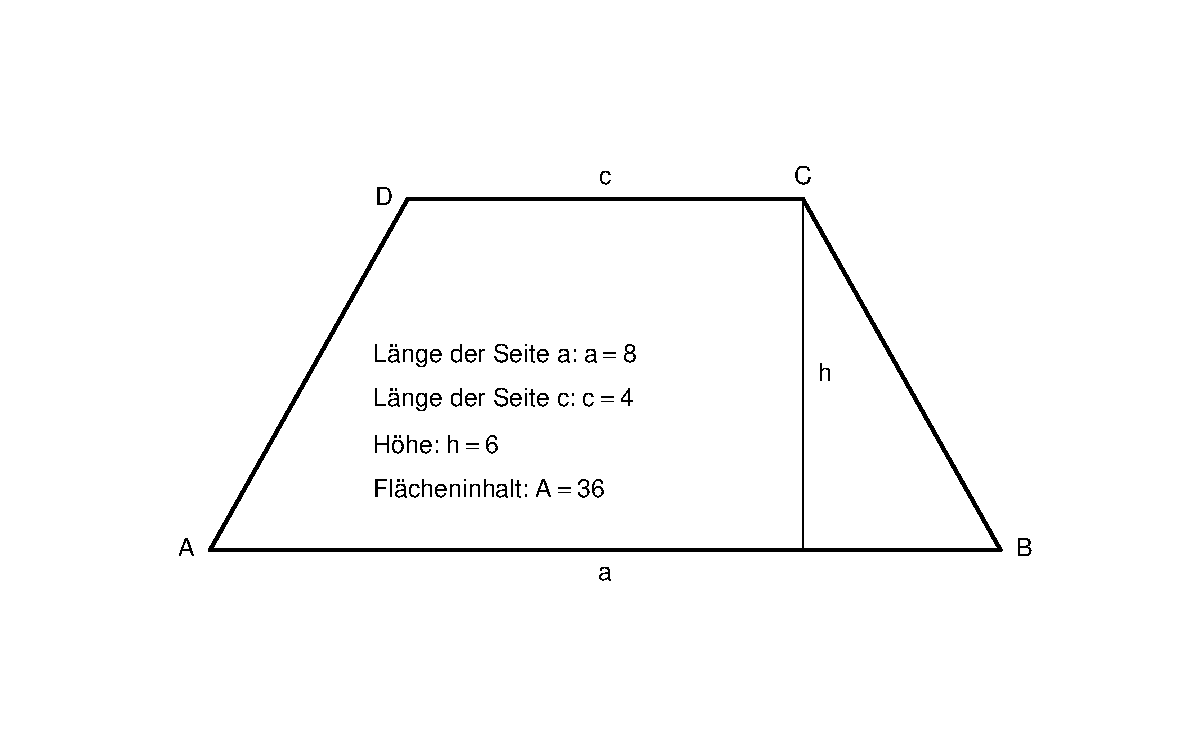
\includegraphics[width=1\linewidth]{Formeln-und-Flächen-8_files/figure-latex/Trapez-1} \end{center}

\textbf{Flächeninhalt des Trapezes:}

\[A = {(a+c) \cdot h \over 2}\]

\textbf{Umfang des Trapezes:}
\[U = a + b + c + d\]

\textbf{Was heißt das doch gleich?}

Hier einmal in Worten: Den Flächeninhalt \(A\) eines Trapezes erhältst du, indem du die Länge der Höhe \(h\) mit der Summe aus der Länge parallelen Seiten a und c multiplizierst und das Ergebnis durch 2 teilst. Auch hier steht die Höhe auf den Seiten a und c senkrecht.

\hypertarget{aufgaben-3}{%
\section*{Aufgaben}\label{aufgaben-3}}
\addcontentsline{toc}{section}{Aufgaben}

\hypertarget{aufgabe-1-3}{%
\subsubsection*{Aufgabe 1}\label{aufgabe-1-3}}
\addcontentsline{toc}{subsubsection}{Aufgabe 1}

Ein Dreieck habe eine Grundseite \(g\) der Länge 4cm und eine zugehörige Höhe \(h\) der Länge 6cm.
Gib die Höhe eines flächengleichen Trapezes mit den parallelen Seiten \(a = 2cm\) und \(c = 4cm\) an.

Lösung

\textbf{Gesucht}

Die Länge der Höhe eines Trapezes.

\textbf{Gegeben}

Gegeben ist:

\begin{enumerate}
\def\labelenumi{\arabic{enumi}.}
\tightlist
\item
  Ein Dreieck mit der Grundseite \(g = 4cm\) und der zugehörige Höhe \(h = 6cm\). Dieses Dreieck hat denselben Flächeninhalt wie das Trapez, dessen Höhe gesucht ist.
\item
  Die Länge der Seite \(a\) des Trapezes: \(a = 2cm\) und
\item
  die Länge der zur Seite \(a\) parallelen Seite \(c\) des Trapezes: \(c= 4cm\).
\end{enumerate}

Den Flächeninhalt eines Dreiecks berechnet man folgendermaßen:
\[ A = {1 \over 2} \cdot g \cdot h \]

Den Flächeninhalt eines Trapezes berechnet man so:
\[ A = {(a+c) \cdot h \over 2} \]

\textbf{Vorüberlegung}

Das Trapez hat den gleichen Flächeninhalt wie ein Dreieck mit der Grundseite \(g = 4cm\) und der zugehörige Höhe \(h = 6cm\).

Dieses Dreieck den Flächeninhalt:
\[ A = {1 \over 2} \cdot g \cdot h = {1 \over 2} \cdot 4 cm \cdot 6 cm = 12 cm² \]
Gesucht ist also die Länge der Höhe \(h\) eines Trapezes mit Flächeninhalt 12 cm² und den parallelen Seiten \(a = 2cm\) und \(c = 4cm\).

\textbf{Einsetzen}

Nun setzen wir alle bekannten Größen ein, das führt zu:
\[ 12 cm² = {(2cm + 4 cm) \cdot h \over 2} \]

\textbf{Auflösen}

Diese Gleichung muss man nach \(h\) auflösen:
\[ \begin{align} 12 cm² &= {(2cm + 4 cm) \cdot h \over 2}\\
{}\\
12cm² &= {6cm \cdot h \over 2} \\
{}\\
12cm² &= 3cm \cdot h \quad\quad |:3cm\\
{}\\
4cm &=h\end{align} \]

\textbf{Antwort}

Die Höhe eines flächengleichen Trapezes muss also 4 cm lang sein.¸

\hypertarget{section-10}{%
\subsubsection*{}\label{section-10}}
\addcontentsline{toc}{subsubsection}{}

\hypertarget{aufgabe-2-3}{%
\subsubsection*{Aufgabe 2}\label{aufgabe-2-3}}
\addcontentsline{toc}{subsubsection}{Aufgabe 2}

Ein Trapez hat den Flächeninhalt 1m². Die Höhe beträgt 20cm. Gib drei verschiedene Möglichkeiten für die Länge der zueinander parallelen Seiten an.

Lösung

\textbf{Gesucht}

Die Längen der parallelen Seiten \(a\) und \(c\).

\textbf{Gegeben}

Gegeben ist:

\begin{enumerate}
\def\labelenumi{\arabic{enumi}.}
\tightlist
\item
  Der Flächeninhalt: \(A=1m²\) und
\item
  die Höhe \(h=20cm\)
\end{enumerate}

Den Flächeninhalt eines Trapezes berechnet man folgendermaßen:
\[A = {(a+c) \cdot h \over 2}\]

\textbf{Einsetzen}

Setzt man nun alle bekannten Größen ein, erhält man folgenden Gleichung:
\[1 m² = {(a+c) \cdot 0,2 m \over 2}\]

\textbf{Auflösen}

Diese Gleichung muss man nach \((a+c)\) auflösen:
\[\begin{align}1 m² &= {(a+c) \cdot 0,2 m \over 2} \\
{}\\
1 m² &= (a+c) \cdot 0,1 m \quad\quad\quad |:0,1m\\
{}\\
10 m &=a+c
\end{align}\]

\textbf{Antwort}

Daraus ergeben sich zum Beispiel folgende Längen für die Seiten a und c:

\begin{enumerate}
\def\labelenumi{\arabic{enumi}.}
\item
  Möglichkeit: Die Seite a ist einen Meter lang, die Seite c neun Meter (denn 1+9=10)
\item
  Möglichkeit: Die Seite a ist zwei Meter lang, die Seite c acht Meter (denn 2+8=10)
\item
  Möglichkeit: Die Seite a ist drei Meter lang, die Seite c sieben Meter (denn 3+7=10)
\end{enumerate}

\hypertarget{section-11}{%
\subsubsection*{}\label{section-11}}
\addcontentsline{toc}{subsubsection}{}

\hypertarget{aufgabe-3-3}{%
\subsubsection*{Aufgabe 3}\label{aufgabe-3-3}}
\addcontentsline{toc}{subsubsection}{Aufgabe 3}

Bei einem Trapez beträgt der Flächeninhalt \(A=12cm²\) und die Höhe \(h=1,5cm\). die zu \(a\) parallele Seite \(c\) ist dreimal so lang wie \(a\). Berechne \(a\) und \(c\).

Lösung

\textbf{Gesucht}

Die Längen der Seiten \(a\) und \(c\).

\textbf{Gegeben}

Gegeben ist:

\begin{enumerate}
\def\labelenumi{\arabic{enumi}.}
\tightlist
\item
  Der Flächeninhalt: \(A=12cm²\) ,
\item
  die Höhe \(h=1,5cm\) und
\item
  der Hinweis, dass die Seite \(c\) dreimal so lang ist wie die Seite \(a\), also: \(c= 3 \cdot a\).
\end{enumerate}

Den Flächeninhalt eines Trapezes berechnet man folgendermaßen:
\[A = {(a+c) \cdot h \over 2}\]

\textbf{Einsetzen}

Setzt man nun alle Angaben ein, erhält man folgenden Gleichung:
\[12 cm² = {(a+3a) \cdot 1,5cm \over 2}\]

\textbf{Auflösen}

Diese Gleichung muss man jetzt nach \(a\) auflösen:

\[ \begin{align}
12 cm² &= {(a+3a) \cdot 1,5cm \over 2}\\
{}\\
12 cm² &= {4a \cdot 1,5 cm \over 2}\\
{}\\
12 cm² &= {a \cdot 6cm \over 2} \\
{}\\
12 cm² &= a \cdot 3cm \quad\quad\quad |:3cm \\
{}\\
4cm &= a \\
{}\\
\Rightarrow a &= 4cm\\
\Rightarrow c &= 3 \cdot a = 3 \cdot 4cm = 12 cm
\end{align}\]

\textbf{Antwort}

Die Seite a ist also 4cm lang, die Länge der Seite c beträgt 12cm.

\hypertarget{section-12}{%
\subsubsection*{}\label{section-12}}
\addcontentsline{toc}{subsubsection}{}

\hypertarget{aufgabe-4-2}{%
\subsubsection*{Aufgabe 4}\label{aufgabe-4-2}}
\addcontentsline{toc}{subsubsection}{Aufgabe 4}

\begin{enumerate}
\def\labelenumi{\alph{enumi})}
\tightlist
\item
  Berechne die Länge der Höhe eines Trapezes mit dem Flächeninhalt \(A=24cm²\) und den parallelen Seiten \(a=6cm\) und \(c=10cm\).
\item
  Gib an, wie man allgemein die Höhe eines Trapezes mit dem parallelen Seiten \(a\) und \(c\) berechnen kann, wenn der Flächeninhalt gegeben ist.
  {[}Mit anderen Worten: Löse die Formel für den Flächeninhalt eines Trapezes nach h auf!{]}
\end{enumerate}

Lösung

\textbf{a)}

\textbf{Gesucht}

Gesucht ist die Länge der Höhe \(h\) eines Trapezes.

\textbf{Gegeben}

Gegeben ist:

\begin{enumerate}
\def\labelenumi{\arabic{enumi}.}
\tightlist
\item
  Der Flächeninhalt: \(A=24cm²\),
\item
  die Seite \(a=6cm\) und
\item
  die dazu parallele Seite \(c=10cm\).
\end{enumerate}

Den Flächeninhalt eines Trapezes berechnet man folgendermaßen:
\[ A = {(a+c) \cdot h \over 2} \]

\textbf{Einsetzen}

Nun setzen wir alle bekannten Größen ein, das führt zu:
\[ 24 cm² = {(6cm + 10 cm) \cdot h \over 2} \]

\textbf{Auflösen}

Diese Gleichung muss man nach \(h\) auflösen:
\[ \begin{align} 24 cm² &= {(6cm + 10 cm) \cdot h \over 2}\\
{}\\
24cm² &= {16cm \cdot h \over 2} \\
{}\\
24cm² &= 8cm \cdot h \quad\quad |:8cm\\
{}\\
3cm &=h\end{align} \]

\textbf{Antwort}

Die Höhe des Trapezes muss also \(3cm\) lang sein.¸

\textbf{b)}

Den Flächeninhalt eines Trapezes berechnet man folgendermaßen:
\[ A = {(a+c) \cdot h \over 2} \]

Diese Gleichung muss man nun nach \(h\) auflösen:
\[\begin{align} A \quad &= {(a+c) \cdot h \over 2} \quad\quad | \cdot 2\\
          {}\\
        2 \cdot A &= (a+c) \cdot h \quad\quad |:(a+c) \\
          {}\\
        {2 \cdot A} \over {a+c} &= \quad h
\end{align}\]

Somit ergibt sich für die Höhe \(h\) folgende Gleichung:
\[h = {2 \cdot A \over a+c}\]

\hypertarget{section-13}{%
\subsubsection*{}\label{section-13}}
\addcontentsline{toc}{subsubsection}{}

\hypertarget{aufgabe-5---zusatzaufgabe-2}{%
\subsubsection*{\texorpdfstring{Aufgabe 5 - \textbf{Zusatzaufgabe}}{Aufgabe 5 - Zusatzaufgabe}}\label{aufgabe-5---zusatzaufgabe-2}}
\addcontentsline{toc}{subsubsection}{Aufgabe 5 - \textbf{Zusatzaufgabe}}

Berechne die fehlenden Größen des Trapezes. Welche Trapeze sind Parallelogramme?

\begin{longtable}[]{@{}lllllll@{}}
\toprule
& a) & b) & c) & d) & e) & f)\tabularnewline
\midrule
\endhead
a & \(5\;m\) & \(4\;m\) & & \(20\;cm\) & \(4,6\;cm\) & \(60\;cm\)\tabularnewline
c & \(3\;m\) & & \(35\;cm\) & & \(74\;mm\) & \(6\;dm\)\tabularnewline
h & & \(6\;m\) & \(1\;m\) & \(1,2\;m\) & \(6\;cm\) & \(12\;cm\)\tabularnewline
Flächeninhalt A & \(20\;m^2\) & \(24\;m^2\) & \(1\;m^2\) & \(0,24\;m^2\) & &\tabularnewline
\bottomrule
\end{longtable}

\hypertarget{section-14}{%
\subsubsection*{}\label{section-14}}
\addcontentsline{toc}{subsubsection}{}

\hypertarget{aufgabe-6---zusatzaufgabe-1}{%
\subsubsection*{\texorpdfstring{Aufgabe 6 - \textbf{Zusatzaufgabe}}{Aufgabe 6 - Zusatzaufgabe}}\label{aufgabe-6---zusatzaufgabe-1}}
\addcontentsline{toc}{subsubsection}{Aufgabe 6 - \textbf{Zusatzaufgabe}}

Zeichne das Viereck in ein Koordinatensystem und ermittle dann den Flächeninhalt. Wähle als Achseneinteilung 2 Kästchen = 1 Einheit.

\begin{enumerate}
\def\labelenumi{\alph{enumi})}
\item
  A(0\textbar4); B(3\textbar4); C(1\textbar8); D(0\textbar8)
\item
  A(4\textbar4); B(7\textbar6); C(9\textbar10); D(3\textbar6)
\end{enumerate}

\hypertarget{vieleck}{%
\chapter{Vieleck}\label{vieleck}}

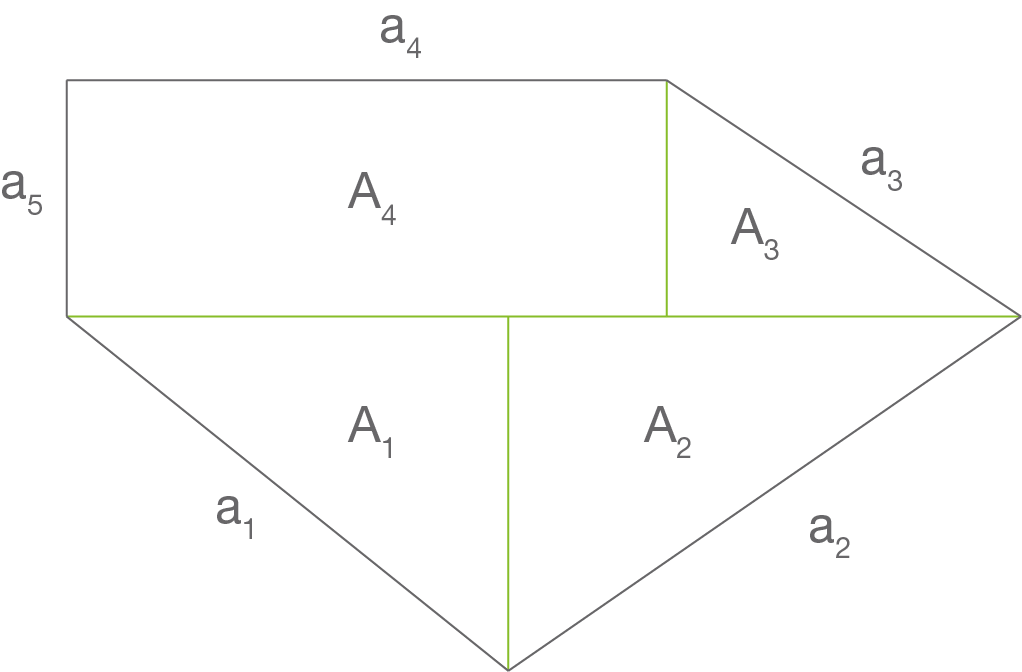
\includegraphics[width=4.16667in,height=\textheight]{./Bilder/VieleckZerlegen.png}

Möchte man den Flächeninhalt eines beliebigen Vielecks bestimmen, so kann man folgendermaßen vorgehen:

\begin{enumerate}
\def\labelenumi{\arabic{enumi}.}
\tightlist
\item
  Zunächst zerlegt man die Vielecksfläche in Teilflächen (Rechtecke, Quadrate, Trapeze, Parallelogramme, Dreiecke), deren Flächeninhalte man berechnen kann.
\item
  Dann berechnet man die Teilflächeninhalte mit Hilfe der entsprechenden Formeln.
\item
  Abschließend bestimmt man den Flächeninhalt des gegebene Vielecks als Summe der Teilflächeninhalte.
\end{enumerate}

\hypertarget{aufgaben-4}{%
\section*{Aufgaben}\label{aufgaben-4}}
\addcontentsline{toc}{section}{Aufgaben}

\hypertarget{aufgabe-1-4}{%
\subsubsection*{Aufgabe 1}\label{aufgabe-1-4}}
\addcontentsline{toc}{subsubsection}{Aufgabe 1}

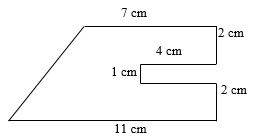
\includegraphics{./Bilder/VieleckA1.jpg}

Berechne den Flächeninhalt.

Lösung

Eine Möglichkeit, den Flächeninhalt zu berechnen, ist, das Vieleck zu einem Trapez zu ergänzen. Anschließend muss dann nur der Flächeninhalt der Ergänzung, also der Flächeninhalt des roten Rechtecks, abgezogen werden.

\textbf{Ergänzung}

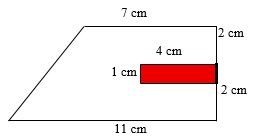
\includegraphics{./Bilder/VieleckL1.png}

\textbf{Berechnung der Trapezfläche}

Für das Trapez gilt:

\begin{itemize}
\tightlist
\item
  \(a= 11 cm\),
\item
  \(c= 7cm\) und
\item
  \(h = 2cm + 1cm + 2cm = 5cm\)
\end{itemize}

Den Flächeninhalt eines Trapezes berechnet man bekanntlich folgendermaßen:
\[A_{Trapez} = {(a+c) \cdot h \over 2}\]

Setzt man alle bekannten Größen ein, ergibt sich folgender Flächeninhalt:
\[ A_{Trapez} = {(11 cm + 7 cm) \cdot 5 cm \over 2} = {18 cm \cdot 5 cm \over 2} = 45 cm²\]

\textbf{Berechnung der Rechtecksfläche}

Das rote Rechteck hat eine

\begin{itemize}
\tightlist
\item
  Länge von \(l = 4cm\) und eine
\item
  Breite von \(b = 1cm\).
\end{itemize}

Den Flächeninhalt eines Rechteck ermittelt man bekanntlich folgendermaßen:
\[A_{Rechteck} = l \cdot b\]\\
Setzt man alle bekannten Größen ein, ergibt sich folgender Flächeninhalt:
\[ A_{Rechteck} = 4 cm \cdot 1cm = 4 cm²\]

\textbf{Berechnung der Vielecksfläche}

Für den Flächeninhalt des Vielecks gilt nun:
\[A_{Vieleck} = A_{Trapez} - A_{Rechteck}\]
Einsetzen der berechneten Flächeninhalte ergibt:
\[A_{Vieleck} = 45cm² - 4cm² =  41cm²\]

\textbf{Antwort}

Die Fläche des Vielecks beträgt \(41cm²\).

\hypertarget{section-15}{%
\subsubsection*{}\label{section-15}}
\addcontentsline{toc}{subsubsection}{}

\hypertarget{aufgabe-2-4}{%
\subsubsection*{Aufgabe 2}\label{aufgabe-2-4}}
\addcontentsline{toc}{subsubsection}{Aufgabe 2}

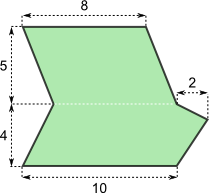
\includegraphics{./Bilder/VieleckA2.png}

Berechne den Flächeninhalt.

Lösung

Eine Möglichkeit, den Flächeninhalt zu berechnen, ist, das Vieleck in ein Parallelogramm, ein Trapez und ein Dreieck zu zerlegen. Der Flächeninhalt des Vielecks ergibt sich dann als die Summe der Teilflächeninhalte.

\textbf{Zerlegung}

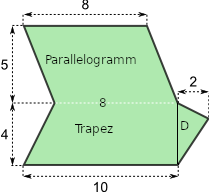
\includegraphics{./Bilder/VieleckL2.png}

\textbf{Der Flächeninhalt des Parallelogramms:}

Für das Parallelogramm gilt:

\begin{itemize}
\tightlist
\item
  \(g= 8\),
\item
  \(h = 5\)
\end{itemize}

Den Flächeninhalt eines Trapezes berechnet man bekanntlich folgendermaßen:
\[A_{Parallelogramm} = g \cdot h\]

Setzt man alle bekannten Größen ein, ergibt sich folgender Flächeninhalt:
\[ A_{Parallelogramm} = 8 \cdot 5 = 40\]

\textbf{Der Flächeninhalt des Trapezes:}

Für das Trapez gilt:

\begin{itemize}
\tightlist
\item
  \(a= 10\),
\item
  \(c= 8\) und
\item
  \(h = 4\)
\end{itemize}

Den Flächeninhalt eines Trapezes berechnet man bekanntlich folgendermaßen:
\[A_{Trapez} = {(a+c) \cdot h \over 2}\]

Setzt man alle bekannten Größen ein, ergibt sich folgender Flächeninhalt:
\[ A_{Trapez} = {(10 + 8) \cdot 4  \over 2} = {18 \cdot 4 \over 2} = 36\]

\textbf{Der Flächeninhalt des Dreiecks:}

Für das Dreieck gilt:

\begin{itemize}
\tightlist
\item
  \(g= 4\),
\item
  \(h = 2\)
\end{itemize}

Den Flächeninhalt eines Dreiecks berechnet man bekanntlich folgendermaßen:
\[A_{Dreieck} = {1 \over 2} \cdot g \cdot h\]

Setzt man alle bekannten Größen ein, ergibt sich folgender Flächeninhalt:
\[ A_{Dreieck} = {1 \over 2} \cdot 4 \cdot 2 = 4\]

\textbf{Der Flächeninhalt des Vielecks:}

Der Flächeninhalt des Vielecks ergibt sich als Summe der Teilflächeninhalte, also:
\[A_{Vieleck} = A_{Parallelogramm} + A_{Trapez} + A_{Dreieck} = 40+36+4 = 80\]

\textbf{Antwort}

Das Vieleck ist \(80\) Quadratflächeneinheiten groß.

\hypertarget{section-16}{%
\subsubsection*{}\label{section-16}}
\addcontentsline{toc}{subsubsection}{}

\hypertarget{aufgabe-3-4}{%
\subsubsection*{Aufgabe 3}\label{aufgabe-3-4}}
\addcontentsline{toc}{subsubsection}{Aufgabe 3}

\begin{center}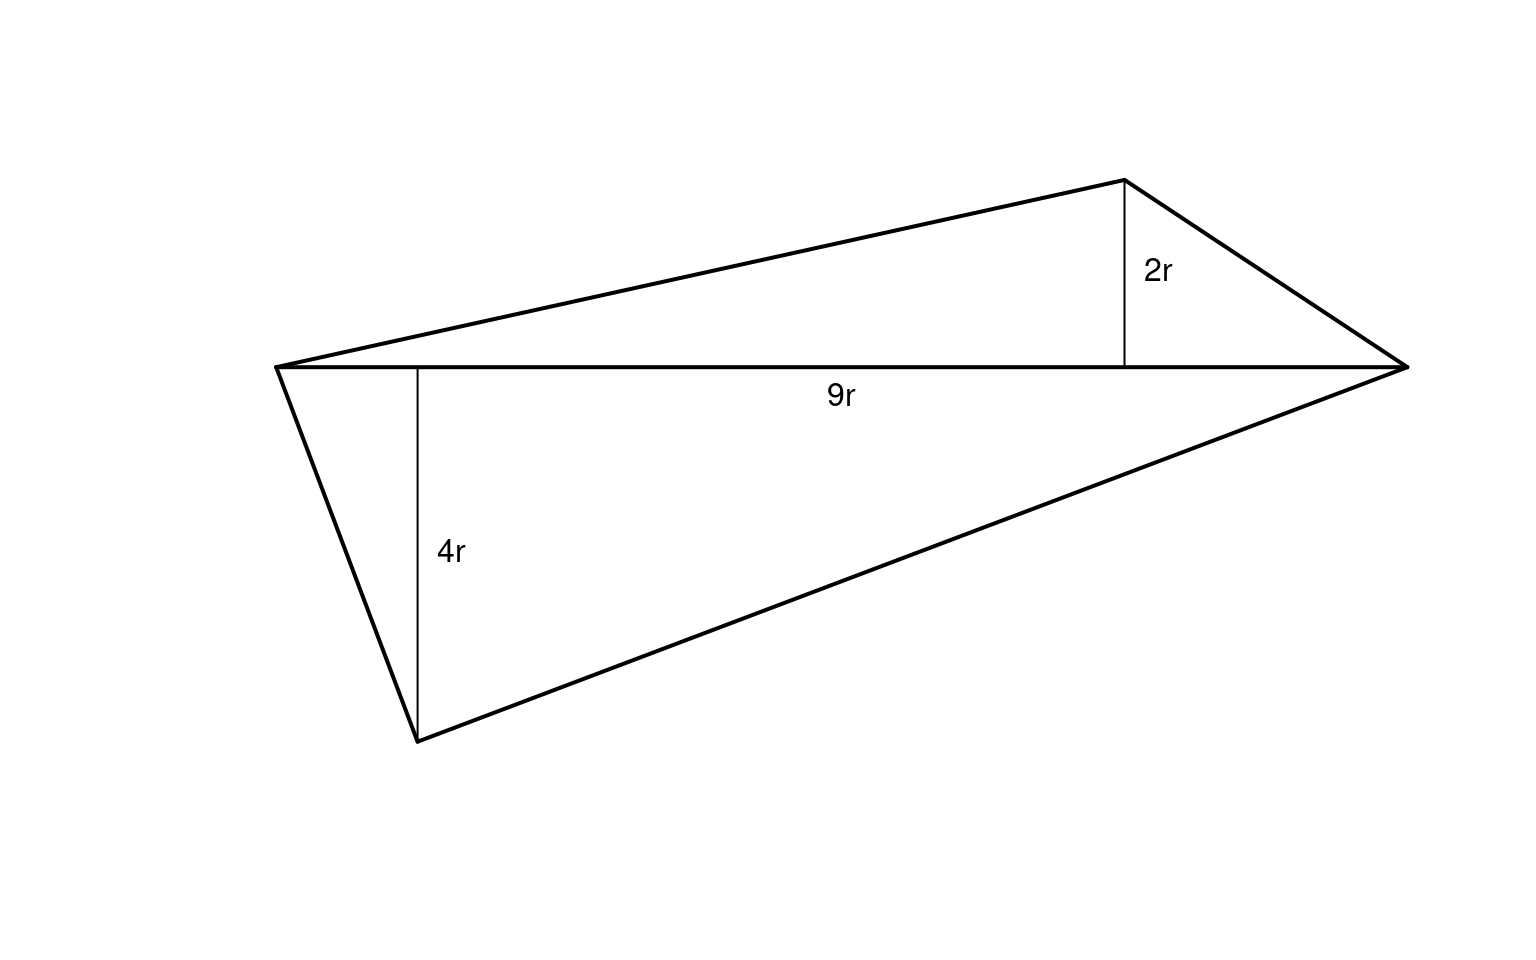
\includegraphics[width=1\linewidth]{Formeln-und-Flächen-8_files/figure-latex/Vieleck-1} \end{center}

Stelle eine Formel auf, mit deren Hilfe man den Flächeninhalt des abgebildeten Vielecks berechnen kan. Vereinfache deine Formel soweit wie möglich!

Lösung

\textbf{Zerlegung}

Ich zerlege das Vieleck in das obere Dreieck mit dem Flächeninhalt \(A_{oberesD}\) und das untere Dreieck mit dem Flächeninhalt \(A_{unteresD}\). Die Summe der beiden Dreieckflächen ergibt den Flächeninhalt des Vielecks.

\textbf{Der Flächeninhalt des oberen Dreiecks}

Für das obere Dreieck gilt:

\begin{itemize}
\tightlist
\item
  \(g= 9r\),
\item
  \(h = r\)
\end{itemize}

Den Flächeninhalt eines Dreiecks berechnet man bekanntlich folgendermaßen:
\[A_{Dreieck} = {1 \over 2} \cdot g \cdot h\]

Setzt man alle bekannten Größen ein, ergibt sich folgender Flächeninhalt:
\[ A_{oberesD} = {1 \over 2} \cdot 9r \cdot 2r = 9r²\]

\textbf{Der Flächeninhalt des unteren Dreiecks}

Für das untere Dreieck gilt:

\begin{itemize}
\tightlist
\item
  \(g= 9r\),
\item
  \(h =4r\)
\end{itemize}

Den Flächeninhalt eines Dreiecks berechnet man bekanntlich folgendermaßen:
\[A_{Dreieck} = {1 \over 2} \cdot g \cdot h\]

Setzt man alle bekannten Größen ein, ergibt sich folgender Flächeninhalt:
\[ A_{unteresD} = {1 \over 2} \cdot 9r \cdot 4r = 18r²\]

\textbf{Der Flächeninhalt des Vielecks}

Der Flächeninhalt des Vielecks ergibt sich als Summe der Teilflächeninhalte, also:
\[A_{Vieleck} = A_{oberesD} + A_{unteresD} = 9r² + 18r² = 27r²\]

\textbf{Antwort}

Das Vieleck ist \(27r²\) Quadratflächeneinheiten groß.

\hypertarget{section-17}{%
\subsubsection*{}\label{section-17}}
\addcontentsline{toc}{subsubsection}{}

\hypertarget{aufgabe-4-3}{%
\subsubsection*{Aufgabe 4}\label{aufgabe-4-3}}
\addcontentsline{toc}{subsubsection}{Aufgabe 4}

\begin{center}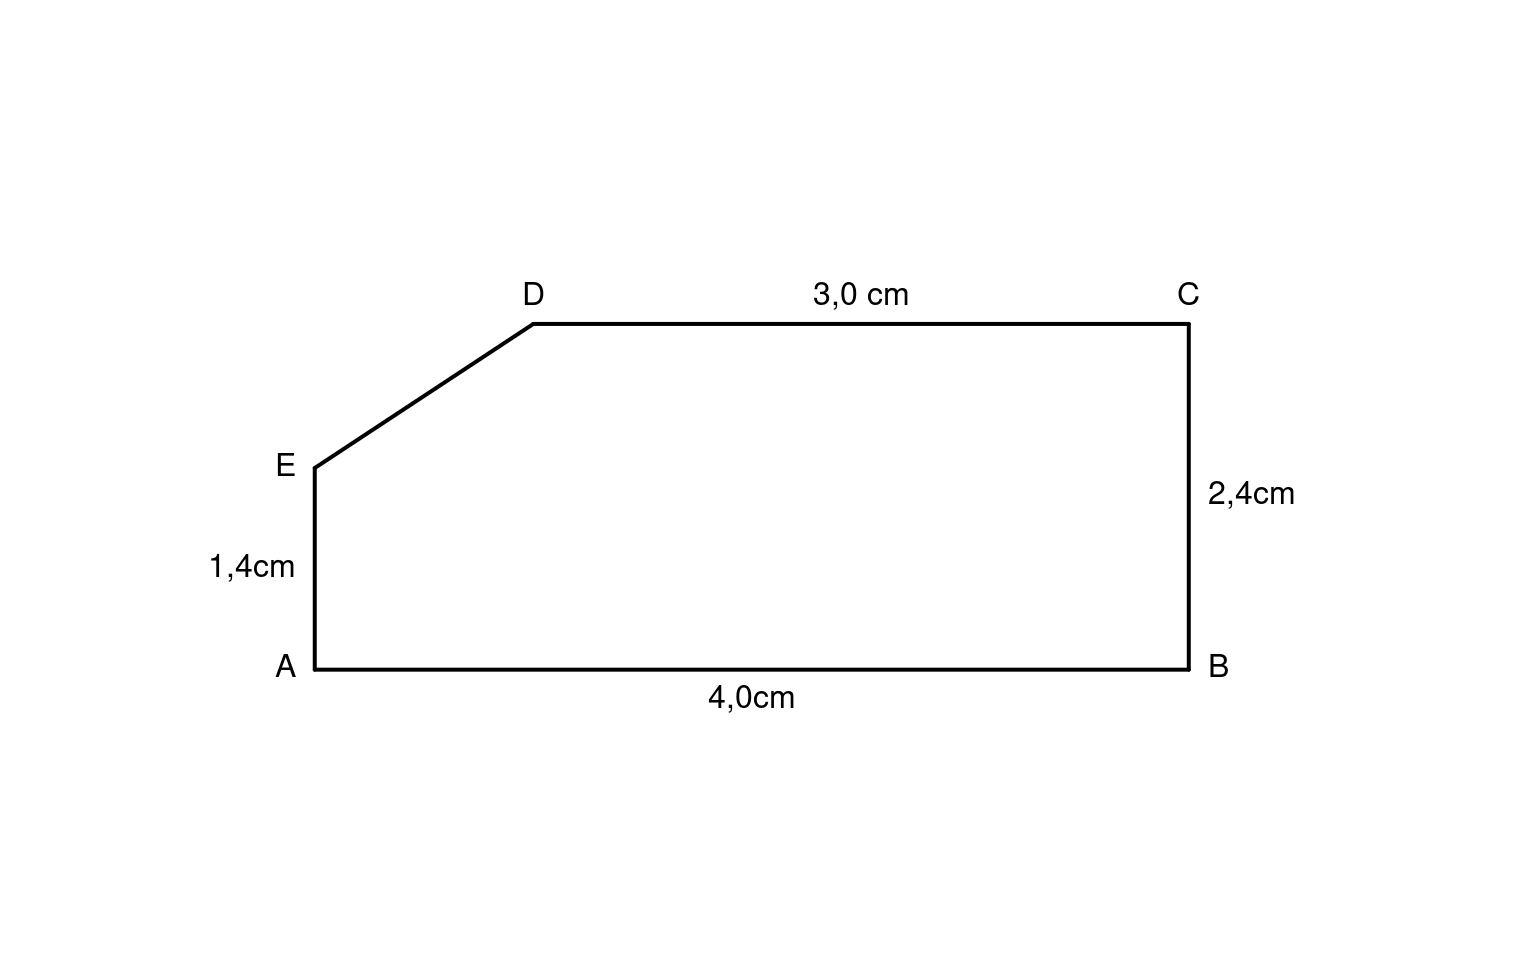
\includegraphics[width=1\linewidth]{Formeln-und-Flächen-8_files/figure-latex/Fuenfeck-1} \end{center}

\begin{enumerate}
\def\labelenumi{\alph{enumi})}
\tightlist
\item
  Berechne den Flächeninhalt des abgebildeten Fünfecks ABCDE.
\end{enumerate}

Lösung

Natürlich gibt es mehr als einen Weg den Flächeninhalt des Fünfecks ABCDE zu berechnen. Man kann oben links ein Dreieck ergänzen

\begin{center}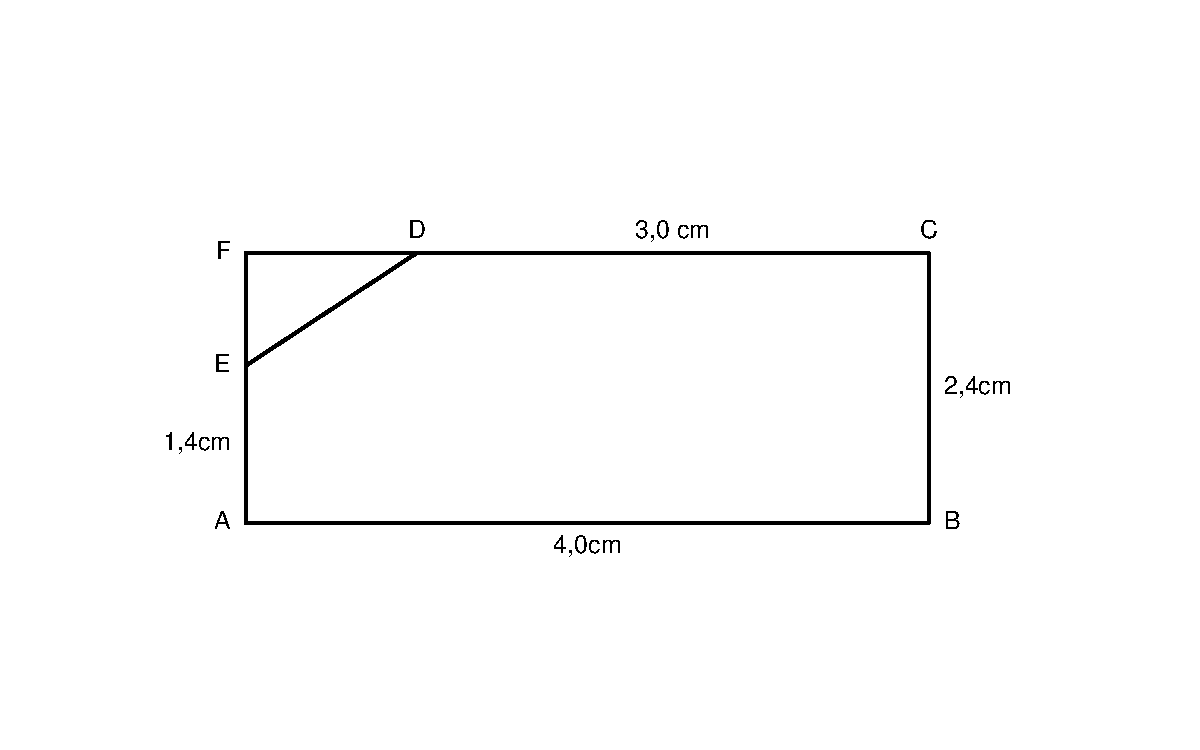
\includegraphics[width=1\linewidth]{Formeln-und-Flächen-8_files/figure-latex/Fuenfeck3-1} \end{center}

oder aber das Fünfeck wie folgt in ein Rechteck und ein Trapez zerlegen.

\begin{center}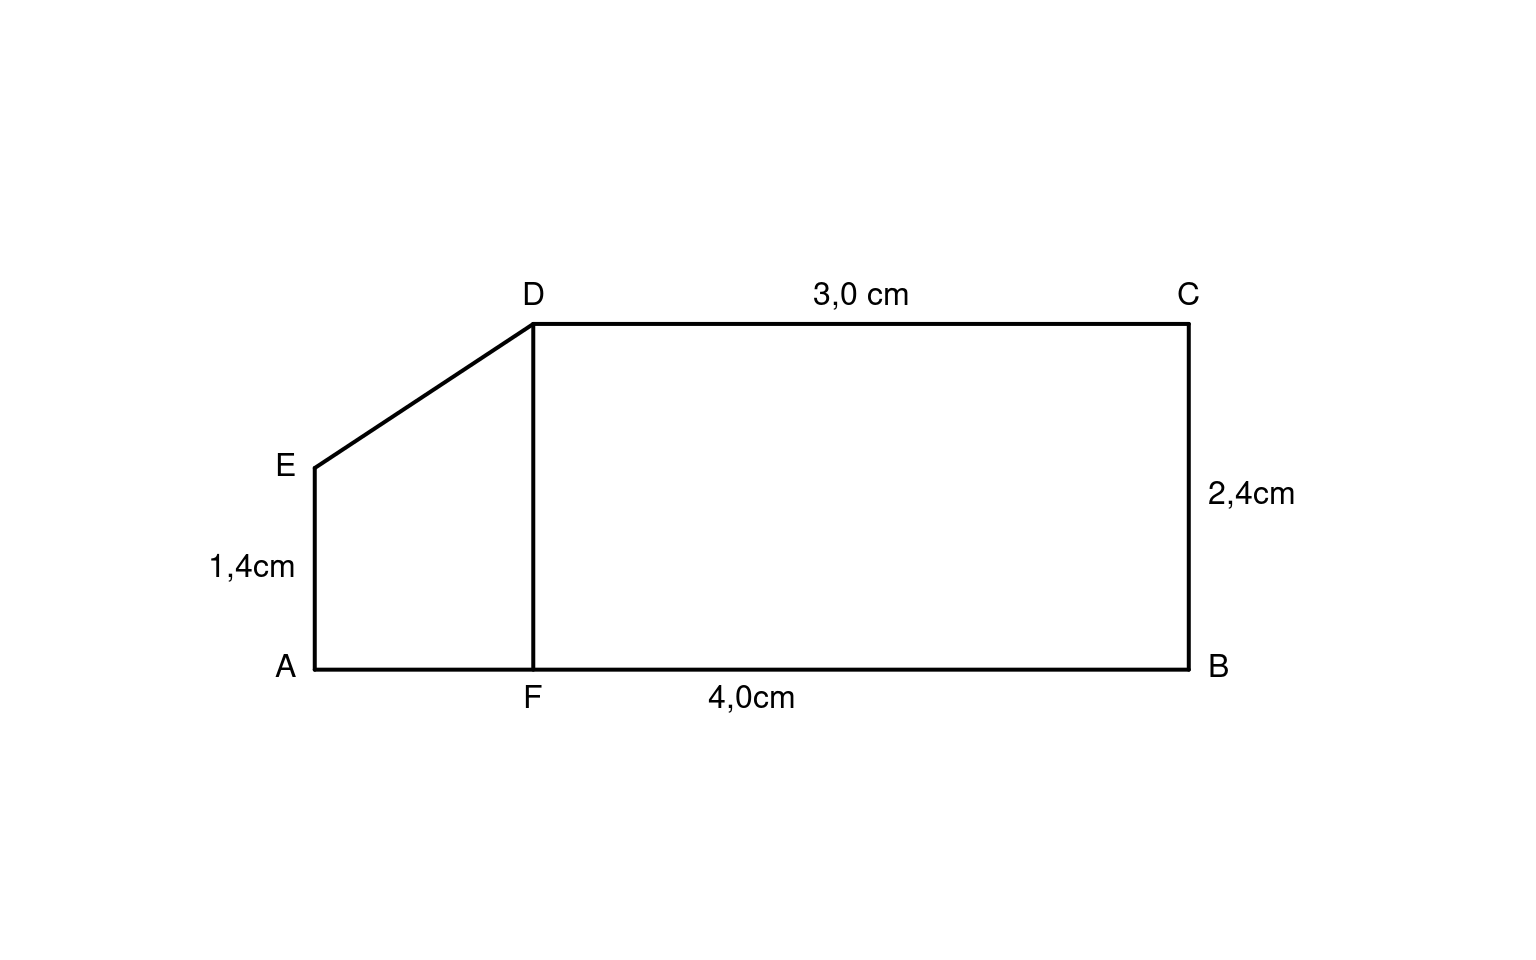
\includegraphics[width=1\linewidth]{Formeln-und-Flächen-8_files/figure-latex/Fuenfeck4-1} \end{center}

Um einmal mehr die Formel für den Flächeninhalt des Trapezes zu verwenden, entscheide ich mich hier für den zweiten Vorschlag: Ich zerlege also das Fünfeck in das Rechteck FBCD und das Trapez AFDE.

Den Flächeninhalt eines Rechtecks berechnet man folgendermaßen:
\[A_R = l \cdot b\]

Für den Flächeninhalt eines Trapezes gilt:
\[A_T = {(a+c) \cdot h \over 2}\]

\textbf{Einsetzen}

Setzt man nun alle bekannten Größen ein, erhält man für den Flächeninhalt des Rechtecks:
\[A_R = 3cm \cdot 2,4cm = 7,2cm²\]
und für den Flächeninhalt des Trapezes:
\[A_T = {(2,4cm+1,4cm) \cdot 1cm \over 2} = 1,9cm²\]
Der Flächeninhalt des Fünfecks ergibt sich nun als die Summe der beiden eben berechneten Flächeninhalte, also:
\[A_F = A_R + A_T = 7,2 cm ² + 1,9 cm² = 9,1cm²\]

\textbf{Antwort}

Das Fünfeck hat einen Flächeninhalt von \(9,1cm²\).

\hypertarget{section-18}{%
\subsubsection*{}\label{section-18}}
\addcontentsline{toc}{subsubsection}{}

\begin{enumerate}
\def\labelenumi{\alph{enumi})}
\setcounter{enumi}{1}
\tightlist
\item
  \textbf{Expertenaufgabe:} Man kann die Ecke E so bewegen, dass der Flächeninhalt des Fünfecks ABCDE unverändert bleibt. Wie ist das möglich?
\end{enumerate}

\hypertarget{section-19}{%
\paragraph*{}\label{section-19}}
\addcontentsline{toc}{paragraph}{}

Tipp 1

Die Diagonale AD zerlegt das Fünfeck in das Viereck ABCD und das Dreieck ADE. Bewegt man nun die Ecke E auf der Parallelen p zu (AD) durch E, so bleibt der Flächeninhalt des Dreiecks ADE immer derselbe. Warum gilt das? Mach dir eine Skizze!

\hypertarget{section-20}{%
\paragraph*{}\label{section-20}}
\addcontentsline{toc}{paragraph}{}

Tipp 2

Betrachte folgende Skizze:

\begin{center}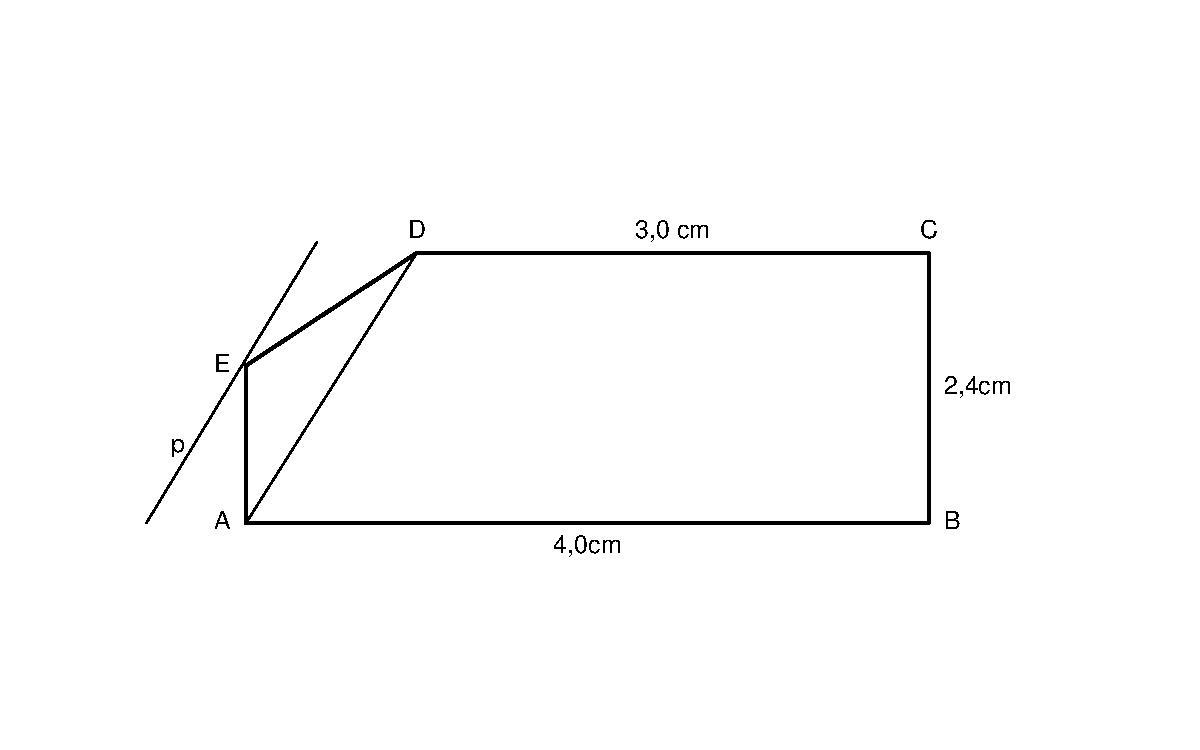
\includegraphics[width=1\linewidth]{Formeln-und-Flächen-8_files/figure-latex/Fuenfeck2-1} \end{center}

Warum bleibt der Flächeninhalt des Dreiecks ADE gleich, unabhängig davon, wohin der Punkt E auf der Geraden p verschoben wird?

\hypertarget{section-21}{%
\paragraph*{}\label{section-21}}
\addcontentsline{toc}{paragraph}{}

Tipp 3

Erinnere dich: Parallele Geraden haben überall denselben Abstand von einander!

\hypertarget{section-22}{%
\paragraph*{}\label{section-22}}
\addcontentsline{toc}{paragraph}{}

Lösung

Betrachte folgende Skizze:

\begin{center}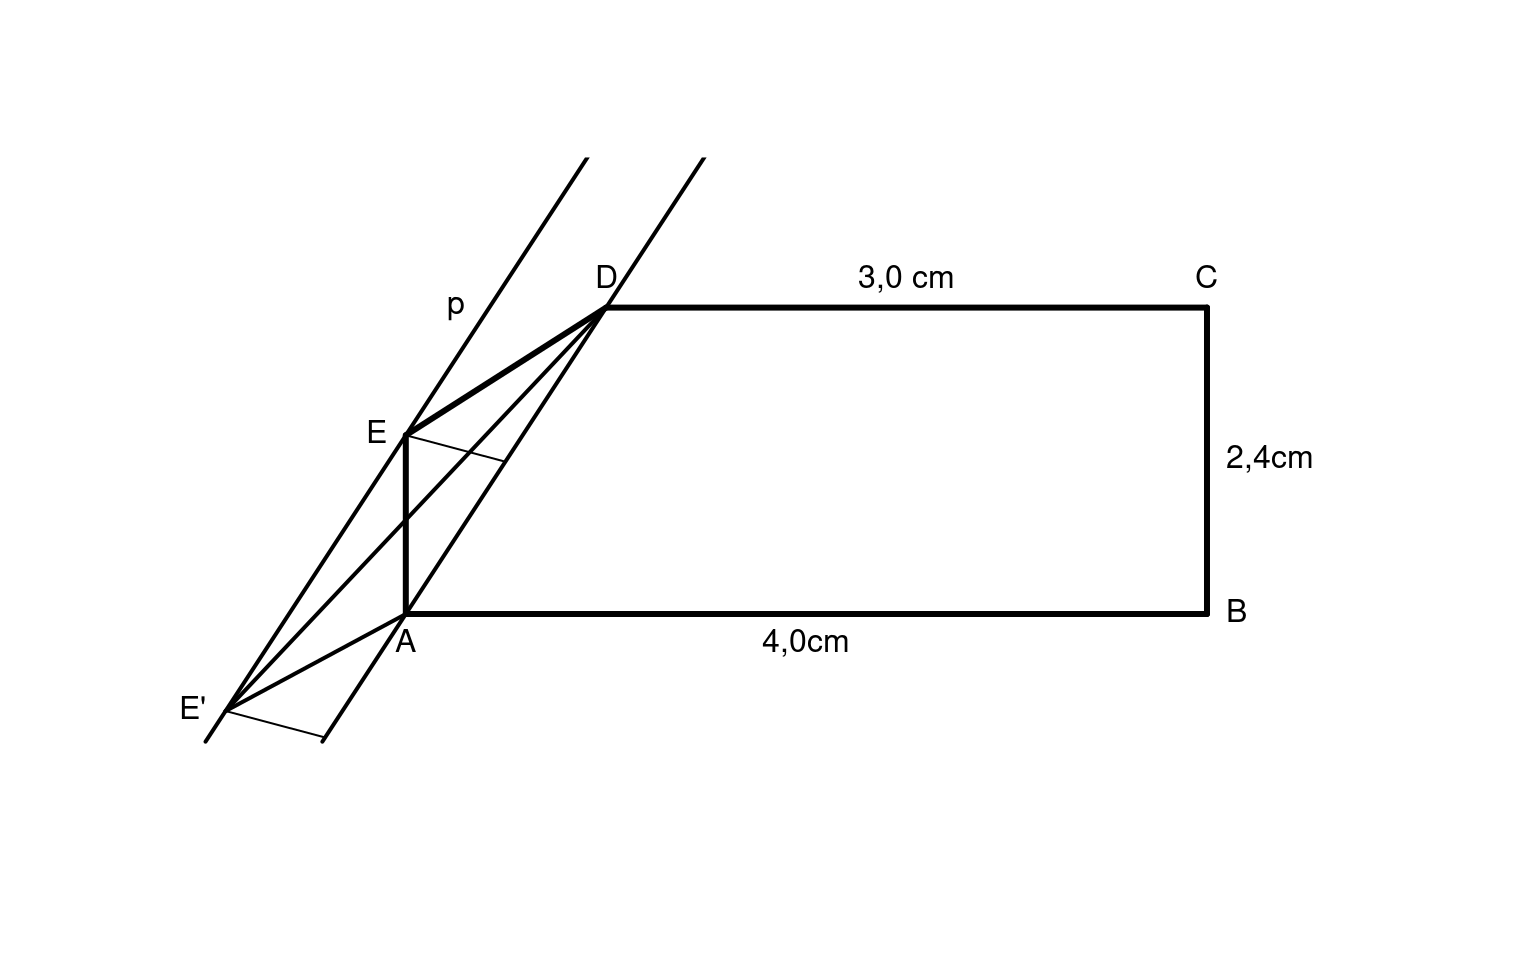
\includegraphics[width=1\linewidth]{Formeln-und-Flächen-8_files/figure-latex/Fuenfeck6-1} \end{center}

Die Diagonale AD zerlegt das Fünfeck in das Viereck ABCD und das Dreieck ADE.

Bewegt man nun die Ecke E auf der durch E verlaufenden und zu (AD) parallelen Geraden p (z.B. nach E'), so bleibt der Flächeninhalt des Dreiecks immer derselbe: Denn parallele Geraden sind bekanntlich immer gleich weit von einander entfernt.
Folglich bleibt die Höhe \(h\) auf die Seite AD immer gleich lang, solange der Punkt E auf der Geraden p verschoben wird.

Da aber auch die Grundlinie AD immer gleich bleibt, ändert sich der Flächeninhalt des Dreiecks nicht, wenn der Punkt auf p verschoben wird.

Der Flächeninhalt des Vierecks ABCD ist unabhängig von E und bleibt deshalb sowieso immer derselbe.

Wenn aber die Flächeninhalte der beiden Teilflächen immer gleich bleiben, so kann sich auch der Flächeninhalt des Fünfecks nicht ändern: Er ergibt sich ja als die Summe der beiden Teilflächeninhalte.

\hypertarget{section-23}{%
\subsubsection*{}\label{section-23}}
\addcontentsline{toc}{subsubsection}{}

\hypertarget{kreis}{%
\chapter{Kreis}\label{kreis}}

Für den Durchmesser \(d\) des Kreises gilt:

Für den Umfang \(U\) des Kreises gilt:

Für den Flächeninhalt gilt:

\(\quad d=2\cdot r\)

\(\quad U= d \cdot \pi\)

\(\quad U = 2 \cdot r \cdot \pi\)

\(\quad A=\pi \cdot r²\)

In diesem Abschnitt dreht sich alles \sout{im} um den Kreis!

\hypertarget{kreisumfang}{%
\section*{Kreisumfang}\label{kreisumfang}}
\addcontentsline{toc}{section}{Kreisumfang}

\begin{figure}
\centering
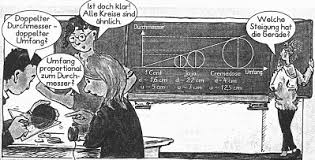
\includegraphics{./Bilder/Umfang.jpeg}
\caption{Das machen wir heute!}
\end{figure}

\hypertarget{kreisuntersuchungen---ein-versuch}{%
\subsubsection*{Kreisuntersuchungen - ein Versuch}\label{kreisuntersuchungen---ein-versuch}}
\addcontentsline{toc}{subsubsection}{Kreisuntersuchungen - ein Versuch}

\begin{quote}
Du brauchst:

\begin{itemize}
\tightlist
\item
  ein Maßband oder eine Stück Schnur und ein Lineal
\item
  ein Blatt Papier und
\item
  einen Bleistift.
\end{itemize}
\end{quote}

\begin{enumerate}
\def\labelenumi{\arabic{enumi}.}
\item
  Geh bitte los und suche verschieden große Gegenstände, die kreisförmig sind bzw. mindestens eine kreisförmige Fläche haben.
\item
  Miss jeweils Umfang und Durchmesser des Kreises und stelle deine Ergebnisse tabellarisch dar.
\end{enumerate}

Eure Messergebnisse

\begin{table}[H]
\centering
\begin{tabular}[t]{l|r|r|r}
\hline
Gegenstand & Durchmesser (cm) & Umfang (cm) & Umfang/Durchmesser\\
\hline
Kerze & 5.5 & 18.0 & 3.272727\\
\hline
Nachttischlampe & 12.0 & 38.0 & 3.166667\\
\hline
Basketball & 25.0 & 75.0 & 3.000000\\
\hline
Spardose & 10.0 & 35.0 & 3.500000\\
\hline
Pringelspackung & 7.5 & 24.5 & 3.266667\\
\hline
Nachttisch & 40.0 & 125.0 & 3.125000\\
\hline
Wasserflasche & 8.0 & 28.5 & 3.562500\\
\hline
Becher & 8.0 & 25.5 & 3.187500\\
\hline
Nutelladeckel & 8.0 & 27.0 & 3.375000\\
\hline
Lampenschirm & 19.0 & 60.0 & 3.157895\\
\hline
Kerze & 7.6 & 24.0 & 3.157895\\
\hline
Glas & 8.0 & 26.0 & 3.250000\\
\hline
Pflanzentopf & 10.0 & 33.0 & 3.300000\\
\hline
Fussball & 21.0 & 66.0 & 3.142857\\
\hline
Flasche & 8.1 & 28.0 & 3.456790\\
\hline
Füller & 1.5 & 15.0 & 10.000000\\
\hline
Handcreme & 3.8 & 12.0 & 3.157895\\
\hline
Kleber & 3.1 & 10.0 & 3.225807\\
\hline
Müslischüssel & 13.0 & 41.0 & 3.153846\\
\hline
Tasse & 6.0 & 21.0 & 3.500000\\
\hline
Schüssel & 13.0 & 38.0 & 2.923077\\
\hline
Spitzer & 3.5 & 14.0 & 4.000000\\
\hline
Dose & 10.0 & 31.5 & 3.150000\\
\hline
Kleber & 3.0 & 10.0 & 3.333333\\
\hline
Kleber 2.0 & 2.0 & 6.5 & 3.250000\\
\hline
Kordel & 4.0 & 13.0 & 3.250000\\
\hline
Stiftehalter & 8.5 & 26.0 & 3.058823\\
\hline
Flasche & 7.0 & 23.0 & 3.285714\\
\hline
Flaschendeckel & 3.0 & 9.5 & 3.166667\\
\hline
Tasse & 9.0 & 20.0 & 2.222222\\
\hline
Blumentopf & 16.0 & 53.5 & 3.343750\\
\hline
Blumentopf 2.0 & 17.5 & 49.0 & 2.800000\\
\hline
Deckel & 6.2 & 16.0 & 2.580645\\
\hline
Münze & 1.8 & 5.5 & 3.055556\\
\hline
Lampenboden & 15.0 & 42.0 & 2.800000\\
\hline
Flaschendeckel & 3.0 & 10.0 & 3.333333\\
\hline
Marmeladenglas & 8.5 & 28.0 & 3.294118\\
\hline
Flaschendeckel & 5.0 & 15.0 & 3.000000\\
\hline
Tasse & 5.0 & 31.0 & 6.200000\\
\hline
Trinkflasche & 6.5 & 21.0 & 3.230769\\
\hline
Glas & 8.5 & 27.5 & 3.235294\\
\hline
Eierbecher & 6.5 & 21.0 & 3.230769\\
\hline
Kölschglas & 5.0 & 17.0 & 3.400000\\
\hline
Deckel & 3.0 & 9.4 & 3.133333\\
\hline
Kleber & 2.5 & 8.5 & 3.400000\\
\hline
Spitzer & 3.7 & 12.8 & 3.459459\\
\hline
Klebeband & 3.3 & 11.5 & 3.484849\\
\hline
Tasse & 9.0 & 26.2 & 2.911111\\
\hline
kleiner Topf & 18.5 & 59.0 & 3.189189\\
\hline
mittlerer Topf & 22.5 & 78.0 & 3.466667\\
\hline
großer Topf & 26.5 & 84.0 & 3.169811\\
\hline
Tasse & 8.5 & 27.0 & 3.176471\\
\hline
Ölflasche & 8.0 & 23.0 & 2.875000\\
\hline
Schälchen & 11.0 & 33.0 & 3.000000\\
\hline
Anspitzer & 4.0 & 15.0 & 3.750000\\
\hline
Klebeband & 9.5 & 30.0 & 3.157895\\
\hline
großer Topf & 22.0 & 64.0 & 2.909091\\
\hline
Griechischer Joghurt & 10.0 & 24.0 & 2.400000\\
\hline
Wasserglas & 8.0 & 26.0 & 3.250000\\
\hline
Tasse & 7.0 & 22.0 & 3.142857\\
\hline
Schüssel & 13.0 & 38.0 & 2.923077\\
\hline
Spitzer & 3.5 & 14.0 & 4.000000\\
\hline
Licht & 4.0 & 13.5 & 3.375000\\
\hline
An-Knopf & 2.0 & 7.0 & 3.500000\\
\hline
Uhr & 4.0 & 13.5 & 3.375000\\
\hline
Spitzer & 3.5 & 13.0 & 3.714286\\
\hline
Lampe & 13.0 & 41.0 & 3.153846\\
\hline
Flasche & 4.5 & 17.0 & 3.777778\\
\hline
Tasse & 8.8 & 29.0 & 3.295454\\
\hline
Packung & 4.5 & 16.0 & 3.555556\\
\hline
Kaffe to go & 7.2 & 24.5 & 3.402778\\
\hline
Lavalam. Deckel & 3.9 & 12.0 & 3.076923\\
\hline
Pfanne & 16.0 & 45.0 & 2.812500\\
\hline
Glas & 7.5 & 26.0 & 3.466667\\
\hline
Tasse & 4.5 & 30.0 & 6.666667\\
\hline
Dose & 7.0 & 34.0 & 4.857143\\
\hline
Deckel & 5.0 & 16.0 & 3.200000\\
\hline
Topf & 21.5 & 67.5 & 3.139535\\
\hline
Glas & 8.0 & 25.5 & 3.187500\\
\hline
Pfanne & 29.5 & 89.0 & 3.016949\\
\hline
kleiner Topf & 15.0 & 48.0 & 3.200000\\
\hline
kleine Pfanne & 26.0 & 76.0 & 2.923077\\
\hline
Tasse & 9.5 & 29.5 & 3.105263\\
\hline
Becher & 10.0 & 35.0 & 3.500000\\
\hline
großer Topf & 25.5 & 76.0 & 2.980392\\
\hline
Duftkerze & 7.1 & 23.3 & 3.281690\\
\hline
Kakteentopf & 6.1 & 21.0 & 3.442623\\
\hline
Trinkflaschenunterseite & 6.3 & 22.0 & 3.492063\\
\hline
Nachttischlampe & 3.2 & 10.3 & 3.218750\\
\hline
Stiftehalter & 8.5 & 26.5 & 3.117647\\
\hline
Spiegel & 17.0 & 47.0 & 2.764706\\
\hline
Müslischale & 12.0 & 35.0 & 2.916667\\
\hline
Tesafilmrolle & 4.0 & 11.0 & 2.750000\\
\hline
Kopf 15 jährige Schwester & 30.0 & 53.0 & 1.766667\\
\hline
Flasche & 9.0 & 25.0 & 2.777778\\
\hline
Kleber 1 & 3.0 & 10.0 & 3.333333\\
\hline
Flasche & 7.0 & 23.5 & 3.357143\\
\hline
Kleber 2 & 2.0 & 6.5 & 3.250000\\
\hline
Tasse & 9.0 & 20.0 & 2.222222\\
\hline
Kordel & 4.0 & 13.0 & 3.250000\\
\hline
Stiftehalter & 8.5 & 26.0 & 3.058823\\
\hline
Flaschendeckel & 3.0 & 9.5 & 3.166667\\
\hline
Blumentopf 1 & 17.5 & 49.0 & 2.800000\\
\hline
Blumentopf 2 & 16.0 & 53.5 & 3.343750\\
\hline
\end{tabular}
\end{table}

\hypertarget{section-24}{%
\subsubsection*{}\label{section-24}}
\addcontentsline{toc}{subsubsection}{}

\begin{table}[H]
\centering
\begin{tabular}[t]{r|r|r}
\hline
Mittelwert Durchmesser (cm) & Mittelwert Umfang (cm) & Mittelwert Umfang/Durchmesser\\
\hline
10.06196 & 31.24674 & 3.150195\\
\hline
\end{tabular}
\end{table}

\begin{enumerate}
\def\labelenumi{\arabic{enumi}.}
\setcounter{enumi}{2}
\tightlist
\item
  Stelle deine Messergebnisse in einem Diagramm dar.
\end{enumerate}

\begin{center}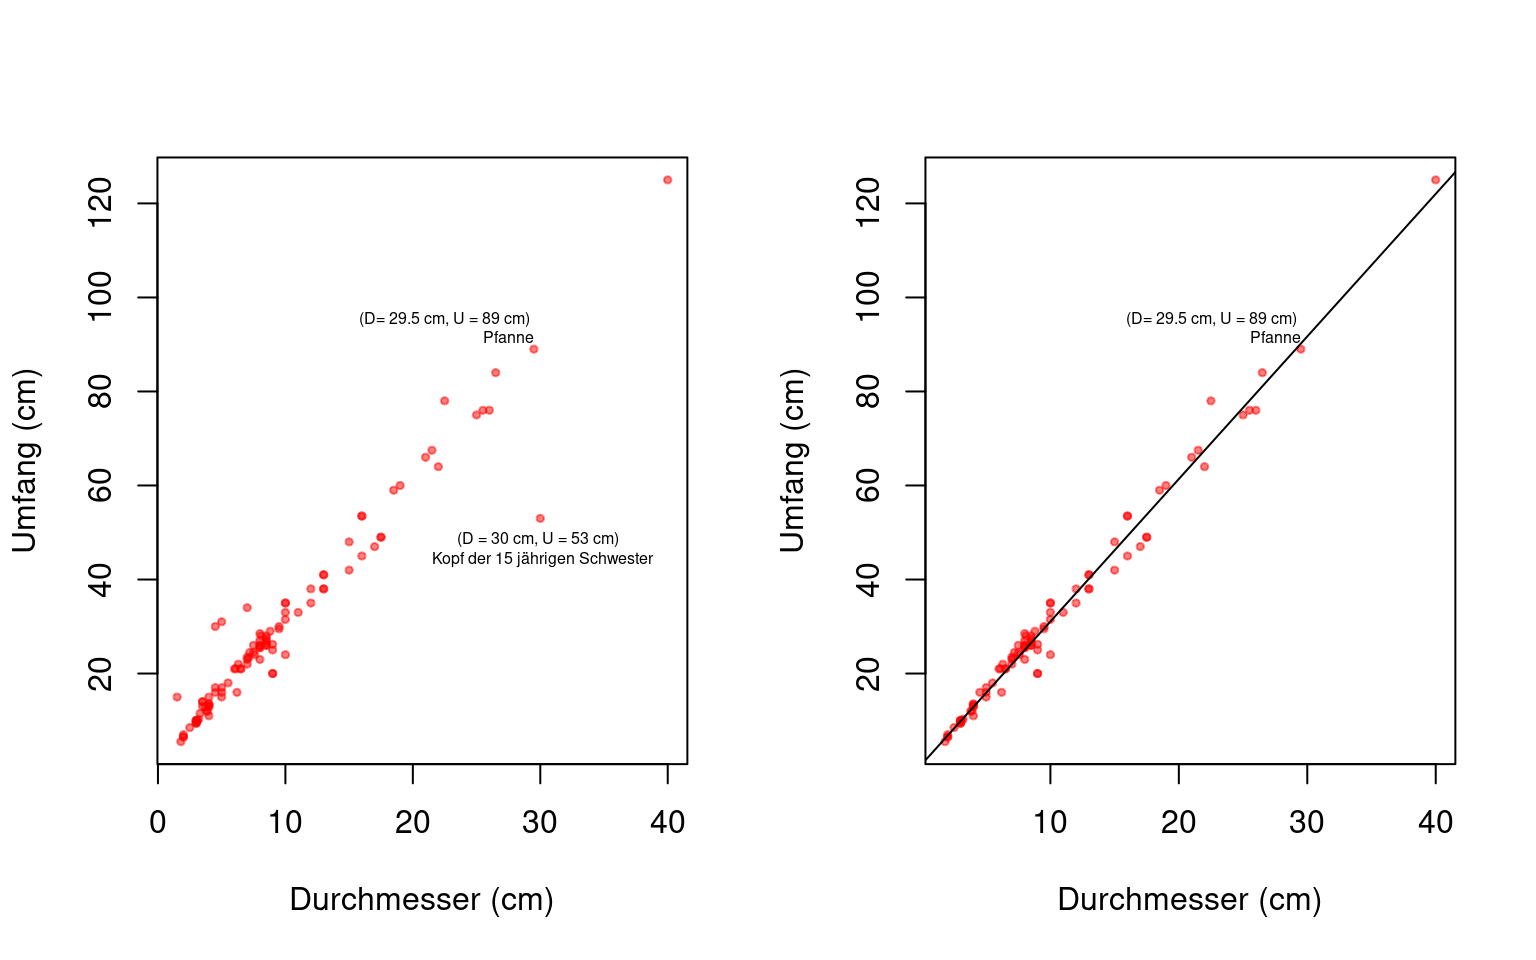
\includegraphics[width=1\linewidth]{Formeln-und-Flächen-8_files/figure-latex/unnamed-chunk-46-1} \end{center}

\hypertarget{zusammenfassung-unserer-ergebnisse}{%
\subsubsection*{Zusammenfassung unserer Ergebnisse}\label{zusammenfassung-unserer-ergebnisse}}
\addcontentsline{toc}{subsubsection}{Zusammenfassung unserer Ergebnisse}

\begin{itemize}
\tightlist
\item
  Unsere Datenpunkte lassen sich gut durch eine Gerade approximieren. Der Umfang eines Kreises wächst also proportional zu seinem Durchmesser.
\item
  Der von uns empirisch ermittelte Proportionalitätsfaktor ist ungefähr 3,15
\item
  Das haben wir gut gemacht.
\end{itemize}

\hypertarget{huxe4tten-wir-keine-messfehler-gemacht-dann}{%
\subsubsection*{Hätten wir keine Messfehler gemacht, dann \ldots{}}\label{huxe4tten-wir-keine-messfehler-gemacht-dann}}
\addcontentsline{toc}{subsubsection}{Hätten wir keine Messfehler gemacht, dann \ldots{}}

\ldots{} hätten wir natürlich den wahren Proportionalitätsfaktor erhalten: \(\pi\).

Es gilt nämlich: \[{U \over d} = \pi\]
oder, wenn man die Gleichung nach \(U\) auflöst:
\[U= \pi \cdot d = \pi \cdot 2 \cdot r\]
Der Durchmesser \(d\) ist ja bekanntlich doppelt so lang wie der Radius \(r\).

\(\pi\) ist eine irrationale Zahl. Ganz exakt lässt sie sich also nicht fassen. Bei den meisten Rechnungen genügt es, als Näherungswert den Wert \(\pi \approx 3,14\) zu verwenden. Euer Taschenrechner kennt \(\pi\).

\hypertarget{kreisfluxe4che}{%
\section*{Kreisfläche}\label{kreisfluxe4che}}
\addcontentsline{toc}{section}{Kreisfläche}

\hypertarget{der-kreisfluxe4che-auf-der-spur---ein-versuchsaufbau}{%
\subsubsection*{Der Kreisfläche auf der Spur - ein Versuchsaufbau}\label{der-kreisfluxe4che-auf-der-spur---ein-versuchsaufbau}}
\addcontentsline{toc}{subsubsection}{Der Kreisfläche auf der Spur - ein Versuchsaufbau}

Der folgende ``mathematische Versuchsaufbau'' soll dir helfen, die Formel für den Flächeninhalt des Kreises herzuleiten und zu verstehen. Probiere also aus, was passiert, wenn du an den gegebenen ``Stellschrauben drehst'' (also die Schieberegler bedienst).

Solltest du Schwierigkeiten bei der Beantwortung der beiden Fragen aus dem ``Versuchsaufbau'' haben, gibt es hier noch drei Tipps:

Tipp 1

Erhöht man die Anzahl der Kreisteile immer mehr, nähert sich die neu angeordnete Fläche einem Rechteck an. Was sind Länge und Breite dieses Rechtecks?

\hypertarget{section-25}{%
\subsubsection*{}\label{section-25}}
\addcontentsline{toc}{subsubsection}{}

Tipp 2

Die Breite des Rechtecks kann man im ``Versuchsaufbau'' ablesen. Sie entspricht dem Radius \(r\) des Kreises. Die Länge des Rechteck muss der halbe Kreisumfang sein. Warum?

\hypertarget{section-26}{%
\subsubsection*{}\label{section-26}}
\addcontentsline{toc}{subsubsection}{}

Tipp 3

Setze die gefundenen Größen:

\begin{itemize}
\tightlist
\item
  Breite des Rechtecks: \(r\) und
\item
  Länge des Rechtecks: \({1 \over 2} \cdot U = {1 \over 2} \pi \cdot 2r\)
\end{itemize}

in die Formel zur Berechung des Flächeninhaltes eines Rechtecks ein und vereinfache diese.

\hypertarget{section-27}{%
\subsubsection*{}\label{section-27}}
\addcontentsline{toc}{subsubsection}{}

\hypertarget{versuchsprotokoll}{%
\subsubsection*{Versuchsprotokoll}\label{versuchsprotokoll}}
\addcontentsline{toc}{subsubsection}{Versuchsprotokoll}

Zunächst zerteilt man den Kreis in gleich große (Kuchen-) Stücke.

Diese ordnet man neu an: Man legt sie so nebeneinander, so dass sie eine annähernd parallelogrammförmige Fläche ergeben. Je größer die Anzahl der Kreisteile wird, desto mehr nähert sich die Fläche einem Rechteck an. Würde man den Kreis in unendlich viele Teile zerschneiden, ergäbe sich schließlich tatsächlich ein Rechteck.

Den Flächeninhalt dieses Rechtecks kann man nun mit der bekannten Formel \(A=l \cdot b\) berechnen.
Die Breite des Rechtecks entspricht dabei dem Radius \(r\), seine Länge dem halben Kreisumfang \({1 \over 2} \cdot U= {1 \over 2} \cdot 2 \cdot \pi \cdot r =\pi \cdot r\).

\hypertarget{ergebnis}{%
\subsubsection*{Ergebnis}\label{ergebnis}}
\addcontentsline{toc}{subsubsection}{Ergebnis}

Damit ergibt sich für die Kreisfläche folgende Formel zur Berechnung des Flächeninhaltes:

\[\begin{align} A &= Länge \cdot Breite\\
{}\\
A &= {1 \over 2} \cdot U \cdot r\\
{}\\
A & ={1 \over 2} \cdot \pi \cdot 2 \cdot r \cdot r\\
{}\\
A & = {1 \over 2} \cdot 2 \cdot \pi \cdot r²\\
{}\\
A &= \pi \cdot r²
\end{align}\]

Für den Flächeninhalt eines Kreises gilt also: \(\quad A= \pi \cdot r²\)

\hypertarget{aufgaben-5}{%
\section*{Aufgaben}\label{aufgaben-5}}
\addcontentsline{toc}{section}{Aufgaben}

\hypertarget{aufgaben-zum-umfang}{%
\subsection*{Aufgaben zum Umfang}\label{aufgaben-zum-umfang}}
\addcontentsline{toc}{subsection}{Aufgaben zum Umfang}

\hypertarget{aufgabe-1-5}{%
\subsubsection*{Aufgabe 1}\label{aufgabe-1-5}}
\addcontentsline{toc}{subsubsection}{Aufgabe 1}

Berechne die fehlenden Größen.

\begin{longtable}[]{@{}llll@{}}
\toprule
& a) & b) & c)\tabularnewline
\midrule
\endhead
Radius \(r\) & \(17cm\) & &\tabularnewline
Durchmesser \(d\) & & & \(9,1 mm\)\tabularnewline
Umfang \(U\) & & \(3,2m\) &\tabularnewline
\bottomrule
\end{longtable}

Lösung

\textbf{Die fehlenden Größen lauten:}

\begin{longtable}[]{@{}llll@{}}
\toprule
& a) & b) & c)\tabularnewline
\midrule
\endhead
Radius \(r\) & \(17cm\) & \(0,509m\) & \(4,55mm\)\tabularnewline
Durchmesser \(d\) & \(34cm\) & \(1,019m\) & \(9,1 mm\)\tabularnewline
Umfang \(U\) & \(106,81cm\) & \(3,2m\) & \(28,59mm\)\tabularnewline
\bottomrule
\end{longtable}

\textbf{Rechnungen:}

\textbf{a)}

\textbf{Durchmesser}

\(d=2 \cdot r = 2 \cdot 17 cm = 34 cm\)

\textbf{Umfang}

\(U = \pi \cdot d = \pi \cdot 34 cm \approx 106,81 cm\)

\textbf{b)}

\textbf{Durchmesser}

Einsetzen führt zu folgender Gleichung:

\(3,2m = \pi \cdot d \quad\)

Auflösen ergibt:

\[ \begin{align} 3,2m &= \pi \cdot d \quad\quad |: \pi \\
{}\\
{3,2m \over \pi} &= d \\
{}\\
\Rightarrow d & \approx 1,019 m
\end{align}\].

\textbf{Radius}

Einsetzen führt zu folgender Gleichung:

\[1,019 m =2 \cdot r\]

Auflösen ergibt:

\[ \begin{align} 1,019 m &=2 \cdot r \quad\quad |: 2 \\
{}\\
{1,019m \over 2} &= r \\
{}\\
\Rightarrow r & \approx 0,509 m
\end{align}\].

\textbf{c)}

\textbf{Umfang}

\(U = \pi \cdot 9,1mm \approx 28,59 mm\)

\textbf{Radius}

Einsetzen führt zu folgender Gleichung:

\[9,1 mm =2 \cdot r\]

Auflösen ergibt:

\[ \begin{align} 9,1 mm &=2 \cdot r \quad\quad |: 2 \\
{}\\
{9,1mm \over 2} &= r \\
{}\\
\Rightarrow r & = 4,55mm
\end{align}\].

\hypertarget{section-28}{%
\subsubsection*{}\label{section-28}}
\addcontentsline{toc}{subsubsection}{}

\hypertarget{aufgabe-2-5}{%
\subsubsection*{Aufgabe 2}\label{aufgabe-2-5}}
\addcontentsline{toc}{subsubsection}{Aufgabe 2}

Walter Hudson, einer der umfangreichsten Männer der Welt, hatte einen Bauchumfang von ca. \(2,80 m\). Passt er durch eine \(80 cm\) breite Tür?

Lösung

\textbf{Vorüberlegung}

Um zu wissen, ob Walter Hudson durch die Tür passt, müsste man seinen Durchmesser kennen.

\textbf{Gegeben}

\begin{enumerate}
\def\labelenumi{\arabic{enumi}.}
\tightlist
\item
  Walter Hudons Bauchumfang mit \(2,80m = 280cm\)
\item
  die Angabe, dass die Tür \(80 cm\) breit ist.
\end{enumerate}

Für den Umfang eines Kreises gilt:

\[ U = \pi \cdot d\].

\textbf{Einsetzen}

Setzt man den gegebenen Bauchumfang ein, ergibt sich folgende Gleichung:
\[ 280 cm = \pi \cdot d \]

\textbf{Auflösen}

Diese Gleichung muss man nach \(d\) auflösen:
\[\begin{align} 280 cm &= \pi \cdot d \quad\quad | : \pi\\
{}\\
{280cm \over \pi } &= d\\
{}\\
\Rightarrow \quad d &\approx 89 cm \quad > 80 cm
\end{align}\]

\textbf{Antwort}

Leider passt Walter Hudson nicht durch die Tür.

\hypertarget{section-29}{%
\subsubsection*{}\label{section-29}}
\addcontentsline{toc}{subsubsection}{}

\hypertarget{aufgabe-3-5}{%
\subsubsection*{Aufgabe 3}\label{aufgabe-3-5}}
\addcontentsline{toc}{subsubsection}{Aufgabe 3}

\begin{enumerate}
\def\labelenumi{\alph{enumi})}
\tightlist
\item
  Der Äquator hat eine Länge von etwa 40000 km. Wie groß ist der Erdradius \(r\)?
\end{enumerate}

Lösung

\textbf{Vorüberlegung}

Die Länge des Äquators entspricht dem Umfang der Erde.

\textbf{Gegeben}

Der Umfang der Erde: \(40000km\)

Für den Umfang eines Kreises gilt:

\[ U = \pi \cdot d\].

\textbf{Einsetzen}

Setzt man den gegebenen Erdumfang ein, ergibt sich folgende Gleichung:
\[ 40000km = \pi \cdot d \]

\textbf{Auflösen}

Diese Gleichung muss man nach \(d\) auflösen:
\[\begin{align} 40000km &= \pi \cdot d \quad\quad | : \pi\\
{}\\
{40000km \over \pi } &= d\\
{}\\
\Rightarrow \quad d &\approx 12732 km
\end{align}\]

Damit folgt für den Erdradius:

\[ r = {1 \over 2} \cdot d = {1 \over 2} \cdot 12732 km \approx 6366 km\]

\hypertarget{section-30}{%
\subsubsection*{}\label{section-30}}
\addcontentsline{toc}{subsubsection}{}

\begin{enumerate}
\def\labelenumi{\alph{enumi})}
\setcounter{enumi}{1}
\tightlist
\item
  Ein 40000 km langes Seil, das am Äquator straff um die Erde gespannt war, wird geringfügig um 1m verlängert und so gestrafft, dass der Abstand von der Erde überall gleich ist. Kannst du jetzt unter diesem Seil hindurchkriechen?
\end{enumerate}

Lösung)

Für den Umfang eines Kreises gilt:

\[U = 2 \cdot \pi \cdot r \]

\textbf{Auflösen}

Auflösen dieser Gleichung nach \(r\) ergibt:

\[ \begin{align} U &= 2 \cdot \pi \cdot r \quad\quad | :2 \pi \\
{}\\
{U \over 2 \cdot \pi} &= r
\end{align}\]

\textbf{Einsetzen}

Setzt man nun die gegebenen Größen ein, ergibt sich:

\[r = {4ooookm + 1m \over 2 \pi} = \underbrace{40000km \over 2\pi}_{Erdradius}+\underbrace{1m \over 2\pi}_{"Zugewinn"}\]

Zum besseren Vorstellen hier noch eine Skizze:

\includegraphics{./Bilder/ÄquatorSeilSkizze.jpeg}

Das Seil steht also \({1 \over 2\pi}m \approx 0,16 cm\) von der Erde ab.

Zumindest ich bin zu groß um darunter durch zu passen \ldots.

\hypertarget{section-31}{%
\subsubsection*{}\label{section-31}}
\addcontentsline{toc}{subsubsection}{}

\hypertarget{aufgabe-4-4}{%
\subsubsection*{Aufgabe 4}\label{aufgabe-4-4}}
\addcontentsline{toc}{subsubsection}{Aufgabe 4}

Die Räder eines Fahrrades haben einen Durchmesser von \(71cm\). Wie viele Umdrehungen macht jedes Rad pro km?

Tipp

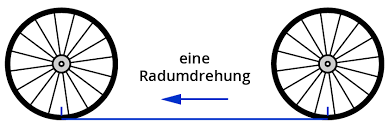
\includegraphics{./Bilder/RadUmdrehung.png}

Wenn sich das Rad einmal ganz dreht, bist du um den Radumfang weitergekommen. Wieviele Umdrehungen passen in einen Kilometer?

\hypertarget{section-32}{%
\subsubsection*{}\label{section-32}}
\addcontentsline{toc}{subsubsection}{}

Lösung

Bei einem Durchmesser von \(71cm\) hat das Rad einen Umfang von

\[U = d \cdot \pi =  71 cm \cdot \pi \approx 223cm = 2,23m\]
In einen Kilometer (\(1000m\)) passen also

\[{1000 m \over 2,23 m} \approx 448,43\]

Radumdrehungen.

\hypertarget{section-33}{%
\subsubsection*{}\label{section-33}}
\addcontentsline{toc}{subsubsection}{}

\hypertarget{section-34}{%
\subsubsection*{}\label{section-34}}
\addcontentsline{toc}{subsubsection}{}

\hypertarget{section-35}{%
\subsubsection*{}\label{section-35}}
\addcontentsline{toc}{subsubsection}{}

\hypertarget{aufgaben-zum-fluxe4cheninhalt}{%
\subsection*{Aufgaben zum Flächeninhalt}\label{aufgaben-zum-fluxe4cheninhalt}}
\addcontentsline{toc}{subsection}{Aufgaben zum Flächeninhalt}

\hypertarget{aufgabe-1-6}{%
\subsubsection*{Aufgabe 1}\label{aufgabe-1-6}}
\addcontentsline{toc}{subsubsection}{Aufgabe 1}

Berechne die fehlenden Größen.

\begin{longtable}[]{@{}llll@{}}
\toprule
& a) & b) & c)\tabularnewline
\midrule
\endhead
Radius \(r\) & & &\tabularnewline
Durchmesser \(d\) & & & \(7,543m\)\tabularnewline
Umfang \(U\) & & \(1,543km\) &\tabularnewline
Flächeninhalt \(A\) & \(13cm²\) & &\tabularnewline
\bottomrule
\end{longtable}

Lösung

\textbf{Die fehlenden Größen lauten:}

\begin{longtable}[]{@{}llll@{}}
\toprule
& a) & b) & c)\tabularnewline
\midrule
\endhead
Radius \(r\) & \(2,034 cm\) & \(0,246 km\) & \(3,772 m\)\tabularnewline
Durchmesser \(d\) & \(4,068 cm\) & \(0,491 km\) & \(7,543m\)\tabularnewline
Umfang \(U\) & \(12,78 cm\) & \(1,543km\) & \(23,70 m\)\tabularnewline
Flächeninhalt \(A\) & \(13cm²\) & \(0,189 km²\) & \(44,69 m²\)\tabularnewline
\bottomrule
\end{longtable}

\textbf{Rechnungen:}

\textbf{a)}

\textbf{Radius}

\(A = \pi \cdot r²\) nach \(r\) auflösen:

\[\begin{align} A &= \pi \cdot r² \quad |:\pi \\
{}\\
{A \over \pi} &= r² \quad |\sqrt{\quad}\\
{}\\
\sqrt{A \over \pi} &= r
\end{align}\]

\(A=13cm²\) einsetzen:

\[\begin{align}r&= \sqrt{13\;cm² \over \pi} \\
{}\\
&\approx 2,034\;cm\end{align}\]

\textbf{Durchmesser}

\[\begin{align} d&=2 \cdot r \\
{}\\
&\approx 2 \cdot 2,034\;cm \\
{}\\
&\approx 4,068\;cm\end{align}\]

\textbf{Umfang}

\[\begin{align} U &= \pi \cdot d \\
{}\\
&\approx \pi \cdot  4,068\;cm \\
{}\\
&\approx 12,78\;cm\end{align}\]

\textbf{b)}

\textbf{Durchmesser}

Die Formel für den Flächeninhalt eines Kreises \(U= \pi \cdot d\) beschreibt den Zusammenhang zwischen Durchmesser und Umfang des Kreises.

Auflösen ergibt:

\[ \begin{align} U &= \pi \cdot d \quad |: \pi \\
{}\\
{U \over \pi} &= d 
\end{align}\].

\(U=1,543 km\) einsetzen:

\[\begin{align} d&={1,543\;km \over \pi}\\ 
{}\\
&\approx 0,491\;km \end{align}\]

\textbf{Radius}

\(d = 2 \cdot r\) nach \(r\) auflösen:

\[\begin{align} d &=2 \cdot r \quad |:2\\
{}\\
{d \over 2} &= r
\end{align}\]

\(0,491 km\) einsetzen:

\[r \approx {0,491 km \over 2} \approx 0,246 km\]

\textbf{Flächeninhalt}

\[\begin{align} A &= \pi \cdot r²\\
{}\\
&\approx \pi \cdot (0,246\;km)² \\
{}\\
&\approx 0,189\;km²\end{align}\]

\textbf{c)}

\textbf{Umfang}

\[\begin{align} U &= \pi \cdot d =\\
{}\\
 &= \pi \cdot 7,543\;m =\\
{}\\
&\approx 23,70\;m \end{align}\]

\textbf{Radius}

\(d = 2 \cdot r\) nach \(r\) auflösen:

\[\begin{align} d &=2 \cdot r \quad |:2\\
{}\\
{d \over 2} &= r
\end{align}\]

\(7,543 m\) einsetzen:

\[\begin{align} r &= {7,543 m \over 2} \\
{}\\
&\approx 3,772\;m \end{align}\]

\textbf{Flächeninhalt}

\[\begin{align} A &= \pi \cdot r² \approx \\
{}\\
&\approx \pi \cdot (3,772 m)²\approx\\
{}\\
&\approx 44,69\;m²\end{align}\]

\hypertarget{section-36}{%
\subsubsection*{}\label{section-36}}
\addcontentsline{toc}{subsubsection}{}

\hypertarget{aufgabe-2-6}{%
\subsubsection*{Aufgabe 2}\label{aufgabe-2-6}}
\addcontentsline{toc}{subsubsection}{Aufgabe 2}

In einer Pizzeria gibt es Pizzen in zwei Größen. Die kleine Pizza hat einen Durchmesser von \(25cm\). Die Fläche der großen Pizza ist doppelt so groß wie die der kleinen Pizza. Berechne den Durchmesser der großen Pizza.

Lösung

\textbf{Gegeben}

\begin{itemize}
\tightlist
\item
  Die kleine Pizza hat den Durchmesser \(d_{klein} = 25 cm\).
\item
  Die Fläche der großen Pizza ist doppelt so groß wie die der kleinen Pizza, also: \(A_{groß}= 2 \cdot A_{klein}\)
\end{itemize}

\textbf{Gesucht}

Der Durchmesser der großen Pizza.

\textbf{Vorgehen}

\(\quad \rightarrow \quad\) Radius der kleinen Pizza ermitteln \(\quad \rightarrow \quad\) Flächeninhalt der kleinen Pizza berechnen \(\quad \rightarrow \quad\) Flächeninhalt der großen Pizza ermitteln \(\quad \rightarrow \quad\) Radius der großen Pizza ermitteln \(\quad \rightarrow \quad\) Durchmesser der großen Pizza berechnen

\textbf{Radius der kleinen Pizza}

\[ r_{klein} = {d_{klein} \over 2} = {25 cm \over 2} = 12,5 cm\]

\textbf{Flächeninhalt der kleinen Pizza}

\[ A_{klein}= \pi \cdot r^2_{klein} = \pi \cdot (12,5cm)² \approx 490,87 cm²\]

\textbf{Flächeninhalt der großen Pizza}

\[A_{groß} = 2 \cdot A_{klein} \approx 981,74 cm²\]

\textbf{Radius der großen Pizza}

\[r_{groß}= \sqrt{A_{groß} \over \pi} \approx \sqrt{312,5cm²} \approx 17,68 cm\]

\textbf{Durchmesser der großen Pizza}

\[d_{groß}= 2 \cdot r_{groß} \approx 35,36 cm\]

\hypertarget{section-37}{%
\subsubsection*{}\label{section-37}}
\addcontentsline{toc}{subsubsection}{}

\hypertarget{aufgabe-3-6}{%
\subsubsection*{Aufgabe 3}\label{aufgabe-3-6}}
\addcontentsline{toc}{subsubsection}{Aufgabe 3}

Untersuche an Zahlenbeispielen und begründe dann allgemein.

\begin{enumerate}
\def\labelenumi{\alph{enumi})}
\tightlist
\item
  Wie verändert sich der Umfang bzw. der Flächeninhalt eines Kreises, wenn sich der Radius verdoppelt?
\end{enumerate}

Lösung

\textbf{Umfang}

Für den Umfang eines Kreises gilt: \(U = 2 \cdot \pi \cdot r\).

Verdoppelt man den Radius (beispielsweise von \(3cm\) auf \(2 \cdot 3cm =6cm\)), setzt man also statt des Radiuses \(r\) den Radius \(2 \cdot r\) in die Formel für den Umfang ein.

Damit erhält man
\[ \begin{align} U_{neu} &= 2 \cdot \pi \cdot (2 \cdot r)= \\
                        {}\\
                         &= 2 \cdot \underbrace{2 \cdot \pi \cdot r}_{= U} =\\
                         {}\\
                         &= 2 \cdot U \end{align}\]

Bei doppeltem Radius verdoppelt sich also der Umfang.

\textbf{Flächeninhalt}

Für den Flächeninhalt eines Kreises gilt: \(A= \pi \cdot r^2\).

Verdoppelt man den Radius (beispielsweise von \(3cm\) auf \(2 \cdot 3cm =6cm\)), setzt man also statt des Radiuses \(r\) den Radius \(2 \cdot r\) in die Formel für den Umfang ein.

Damit erhält man

\[ \begin{align} A_{neu} &= \pi \cdot (2r)^2 =\\
                          {}\\
                         &= \pi \cdot 4\cdot r^2 =\\
                         {}\\
                         &= 4 \cdot \underbrace{\pi \cdot r^2}_{=A} =\\
                         {}\\
                         &= 4 \cdot A \end{align}\]

Bei doppeltem Radius vervierfacht sich also der Flächeninhalt.

\hypertarget{section-38}{%
\subsubsection*{}\label{section-38}}
\addcontentsline{toc}{subsubsection}{}

\begin{enumerate}
\def\labelenumi{\alph{enumi})}
\setcounter{enumi}{1}
\tightlist
\item
  Wie verändert sich der Umfang bzw. der Flächeninhalt eines Kreises, wenn man den Radius um \(10cm\) vergrößert?
\end{enumerate}

Lösung

\textbf{Umfang}

Für den Umfang eines Kreises gilt: \(U = 2 \cdot \pi \cdot r\).

Vergrößert man den Radius eines Kreises um \(10cm\) (z.B. von \(6cm\) auf \(16cm\)), bedeutet dies, dass man in die Formel für den Umfang eines Kreises statt des Radiuses \(r\) den Radius \(r+10cm\) einsetzt.

Damit erhält man

\[ \begin{align} U_{neu} &= 2 \cdot \pi \cdot (r + 10cm) =\\
{}\\
                         &= \underbrace{2 \cdot \pi \cdot r}_{=U} + 2 \cdot \pi \cdot 10cm =\\
                         {}\\
                         &= U + 20\cdot\pi cm \end{align}\]

Erhöht man den Radius um \(10cm\), erhöht sich der Umfang um \(20 \cdot \pi cm\).

\textbf{Flächeninhalt}

Für den Flächeninhalt eines Kreises gilt: \(A= \pi \cdot r^2\).

Vergrößert man den Radius eines Kreises um \(10cm\) (z.B. von \(6cm\) auf \(16cm\)), bedeutet dies, dass man in die Formel für den Flächeninhalt eines Kreises statt des Radiuses \(r\) den Radius \(r+10cm\) einsetzt.

Damit erhält man

\[ \begin{align} A_{neu} &= \pi \cdot (r+10)^2 =\\
{}\\
                         &= \pi \cdot (r^2+2\cdot r \cdot 10 + 100) =\\
                         {}\\
                         &= \pi \cdot (r^2+ r \cdot  20 + 100) =\\
                         {}\\
                         &= \underbrace{\pi \cdot r^2}_{=A} + \pi \cdot r \cdot 20 + \pi \cdot 100 =\\
                         {}\\
                         &= A + 20 \pi \cdot (r+5) \end{align}\]

Erhöht man den Radius um \(10cm\), erhöht sich der Flächeninhalt um \(20 \pi \cdot (r+5)cm²\).

\hypertarget{section-39}{%
\subsubsection*{}\label{section-39}}
\addcontentsline{toc}{subsubsection}{}

\hypertarget{aufgabe-4-5}{%
\subsubsection*{Aufgabe 4}\label{aufgabe-4-5}}
\addcontentsline{toc}{subsubsection}{Aufgabe 4}

Ein kreisrunder Froschteich hat den Radius \(r_1=7m\).

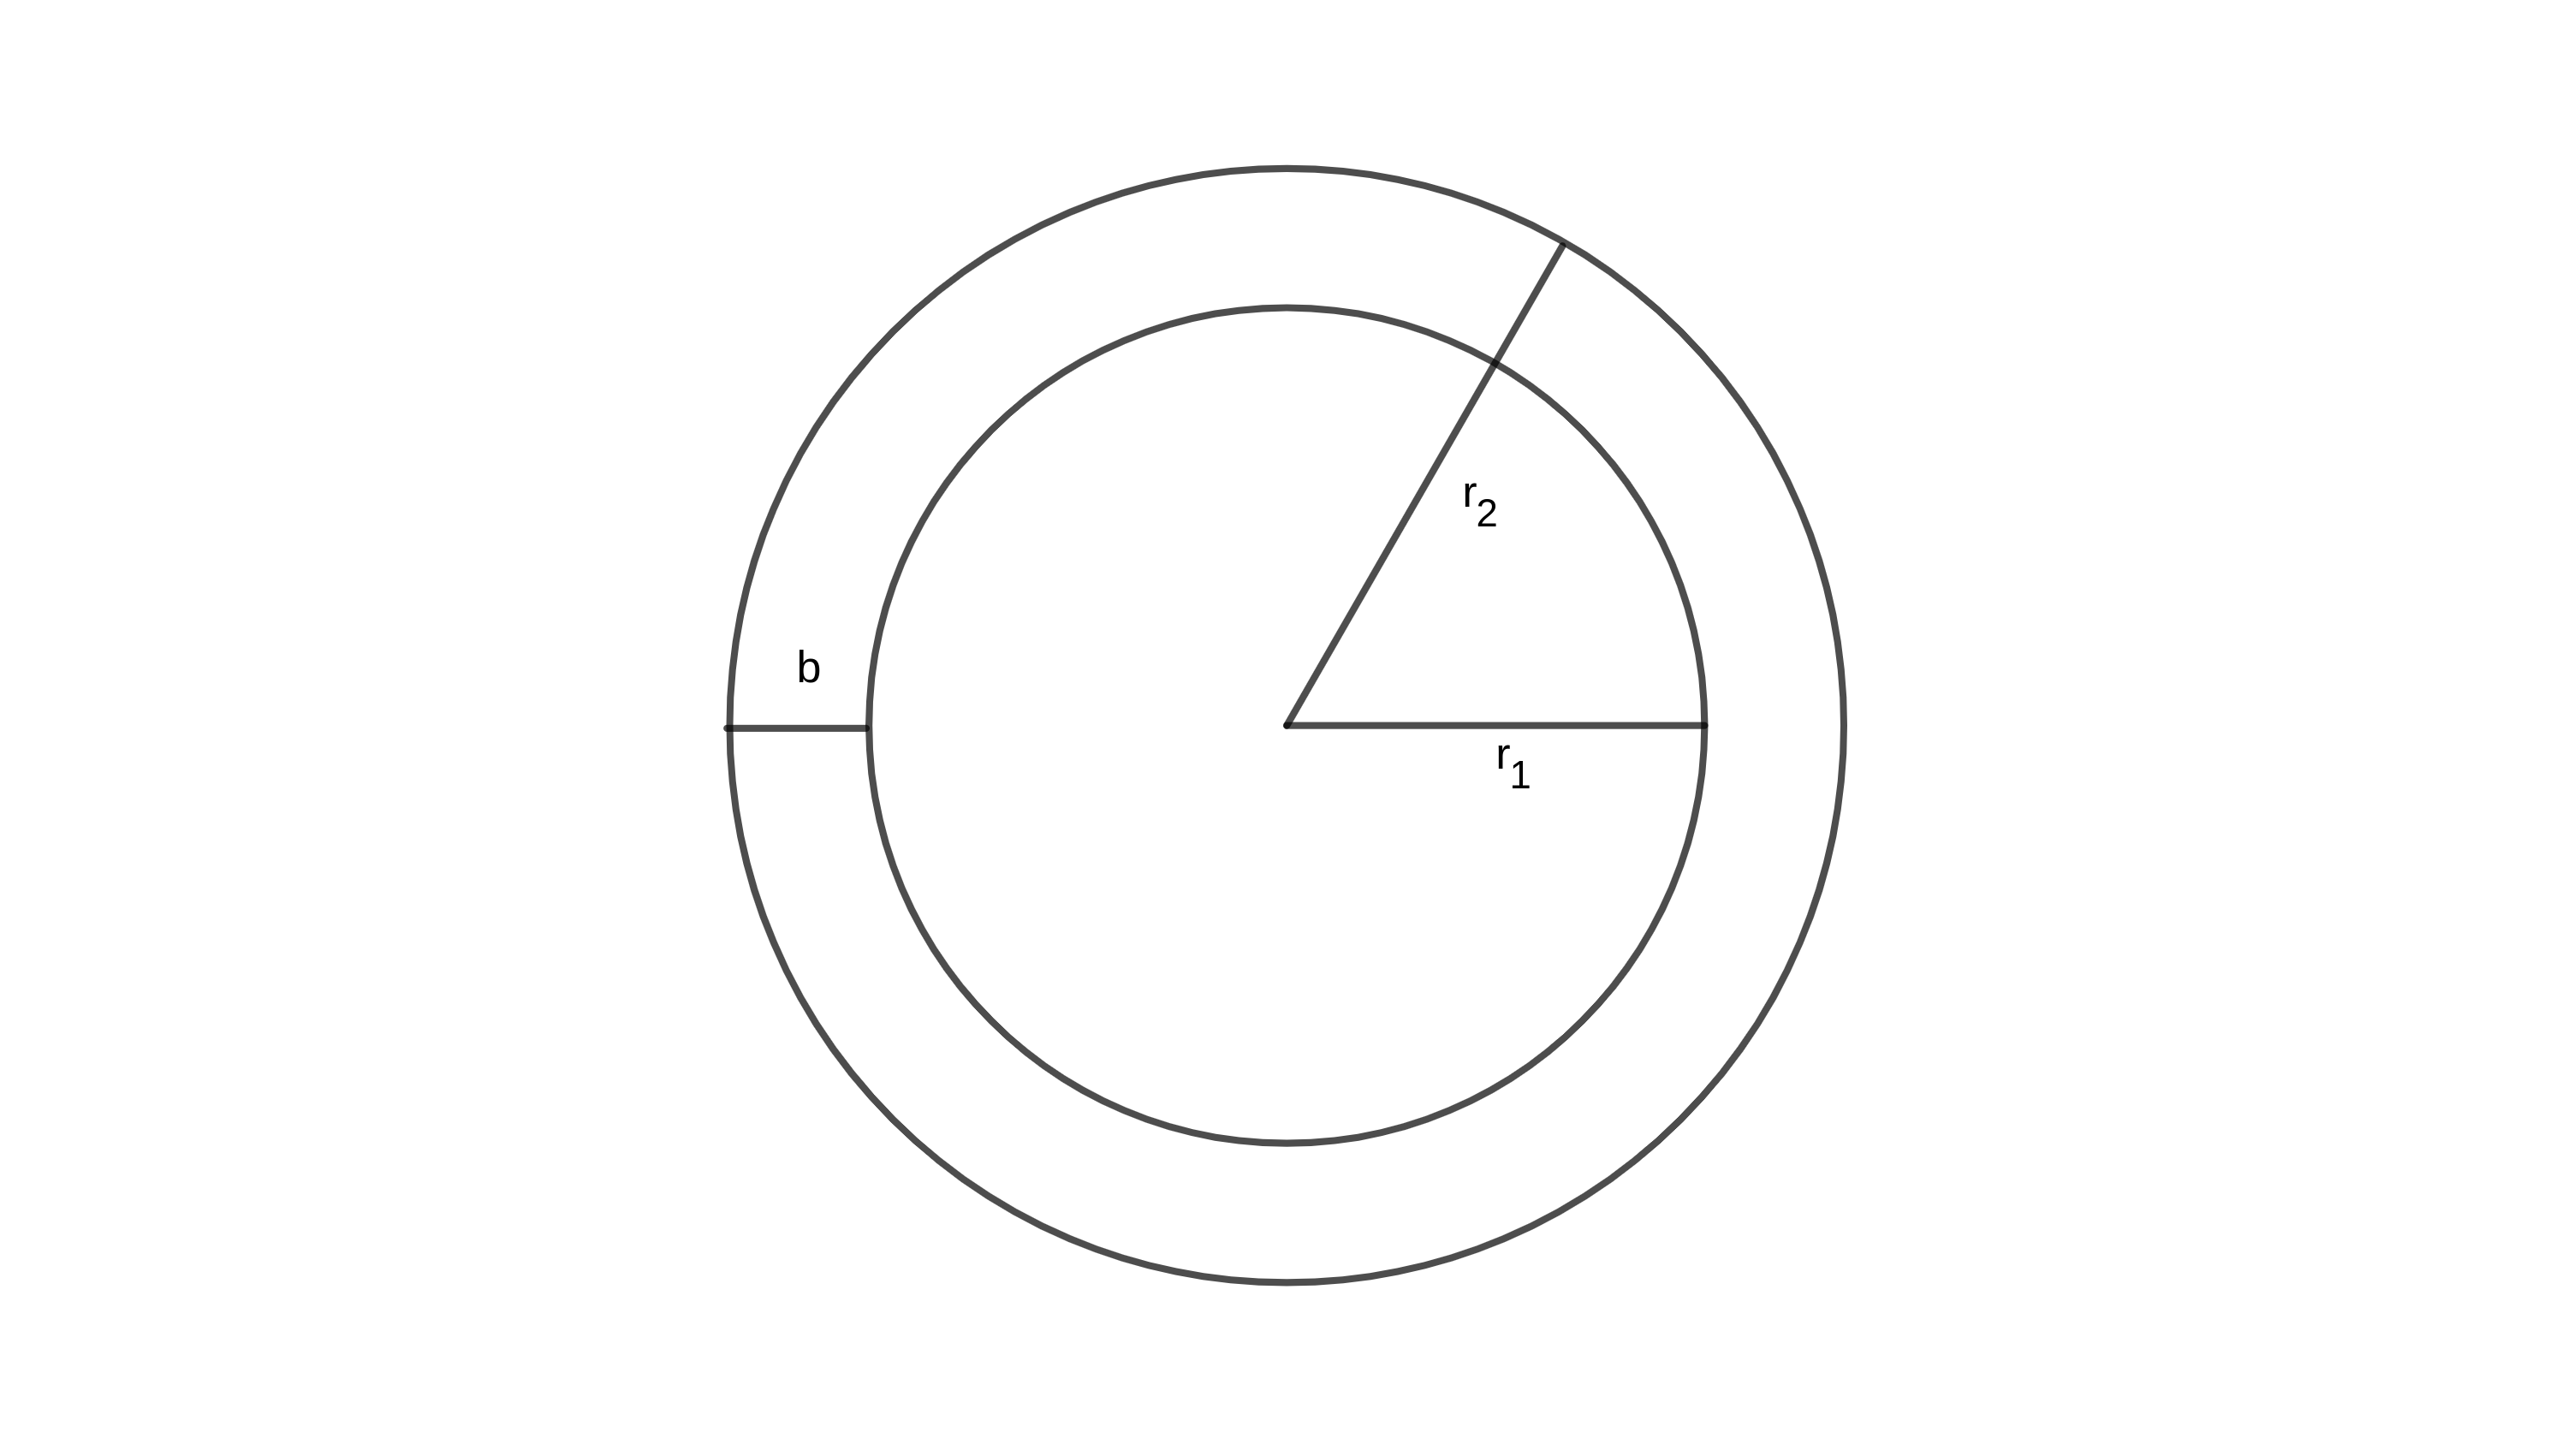
\includegraphics{./Bilder/WegUmTeich.png}

\begin{enumerate}
\def\labelenumi{\alph{enumi})}
\tightlist
\item
  Um den Teich wird ein 3m breiter Weg angelegt. Welchen Flächeninhalt hat der Weg.
\end{enumerate}

Lösung

\textbf{Gegeben}

\begin{itemize}
\tightlist
\item
  Der kleinere Kreis \(k_1\) hat den Radius \(r_1 = 7m\).
\item
  Die Breite \(b\) des Weges beträgt \(3m\). Damit hat der größere Kreis \(k_2\) den Radius \(r_2= 10m\).
\end{itemize}

\textbf{Vorüberlegung}

Zieht man den Flächeninhalt des kleineren Kreises vom Flächeninhalt des größeren Kreises ab, bleibt der Flächeninhalt des Weges übrig. Es gilt also:

\[A_{Weg}=A_{k_2} - A_{k_1}\]

Den Flächeninhalt eines Kreises berechnet man mit der Formel: \(A=\pi \cdot r^2\)

\textbf{Aufstellen der Formel zur Berechnung des Flächeninhaltes des Weges}

\[\begin{align} A_{Weg} &=A_{k_2} - A_{k_1} =\\
                        &= \pi \cdot r^2_2 - \pi \cdot r^2_1 =\\
                        &= \pi \cdot (r^2_2 -r^2_1) \end{align}\]

\textbf{Einsetzen}

\[\begin{align} A_{Weg} &= \pi \cdot (r^2_2 -r^2_1) =\\
                        &=\pi \cdot (100m² - 49m²) =\\
                        &= \pi \cdot 51m² \approx 160,22m² \end{align}\]

\textbf{Antwort}

Der Flächeninhalt des Weges beträgt ca. 160m².

\hypertarget{section-40}{%
\subsubsection*{}\label{section-40}}
\addcontentsline{toc}{subsubsection}{}

\begin{enumerate}
\def\labelenumi{\alph{enumi})}
\setcounter{enumi}{1}
\tightlist
\item
  Wie breit ist der Weg, wenn er einen Flächeninhalt von \(130 m²\) hat?
\end{enumerate}

Lösung

\textbf{Gegeben}

\begin{itemize}
\tightlist
\item
  Der kleinere Kreis \(k_1\) hat den Radius \(r_1 = 7m\).
\item
  Der Weg hat einen Flächeninhalt von \(130 m²\).
\end{itemize}

\textbf{Vorüberlegung}

Die Breite des Weges ergibt sich aus der Differenz der beiden Radien: \(b=r_2 - r_1\).
\(r_1\) ist gegeben, \(r_2\) dagegen muss noch ermittelt werden.

Mit Hilfe des Radiuses \(r_1\) des kleineren Kreises \(k_1\) kann man den Flächeninhalt des kleineren Kreises berechnen: \(A_1 = \pi \cdot r^2_1\). Addiert man zu dieser Fläche die Fläche des Weges \(A_{Weg}\), ergibt sich der Flächeninhalt des größeren Kreises, also \(A_2= A_1+ A_{Weg}\).

Hat man den Flächeninhalt des größeren Kreises, lässt sich der Radius \(r_2\) des größeren Kreises bestimmen.

Für den Radius eines Kreises mit Flächeninhalt \(A\) gilt: \(r = \sqrt{A \over \pi}\).

\textbf{Aufstellen der Formel zur Berechnung der Breite des Weges}
\[ \begin{align} b &= r_2 - r_1 = \\
{}\\
                         &= \sqrt{A_2 \over \pi} - r_1=\\
{}\\
                         &= \sqrt{A_1+  A_{Weg} \over \pi} - r_1= \\
                     {}\\
                     & = \sqrt{\pi \cdot r^2_1+  A_{Weg} \over \pi} - r_1
                     \end{align}\]

\textbf{Einsetzen}

\[ \begin{align} b &=\sqrt{\pi \cdot r^2_1+  A_{Weg} \over \pi} - r_1=\\
{}\\
                    &=\sqrt{\pi \cdot (7m)²+  130m² \over \pi} - 7m \approx\\
                    {}\\
                    & \approx \sqrt{ 283,93804 m² \over \pi} - 7m \approx \\
                    {}\\
                    & \approx \sqrt{90,3802852 m²} - 7m \approx 2,5 m \end{align}\]

\textbf{Antwort}

Der Weg ist ca.\(2,5m\) breit.

\hypertarget{section-41}{%
\subsubsection*{}\label{section-41}}
\addcontentsline{toc}{subsubsection}{}

\hypertarget{aufgabe-5-1}{%
\subsubsection*{Aufgabe 5}\label{aufgabe-5-1}}
\addcontentsline{toc}{subsubsection}{Aufgabe 5}

Aus einer quadratischen Platte mit der Seitenlänge \(a\) wird eine Kreisscheibe herausgeschnitten (vgl. Skizze).

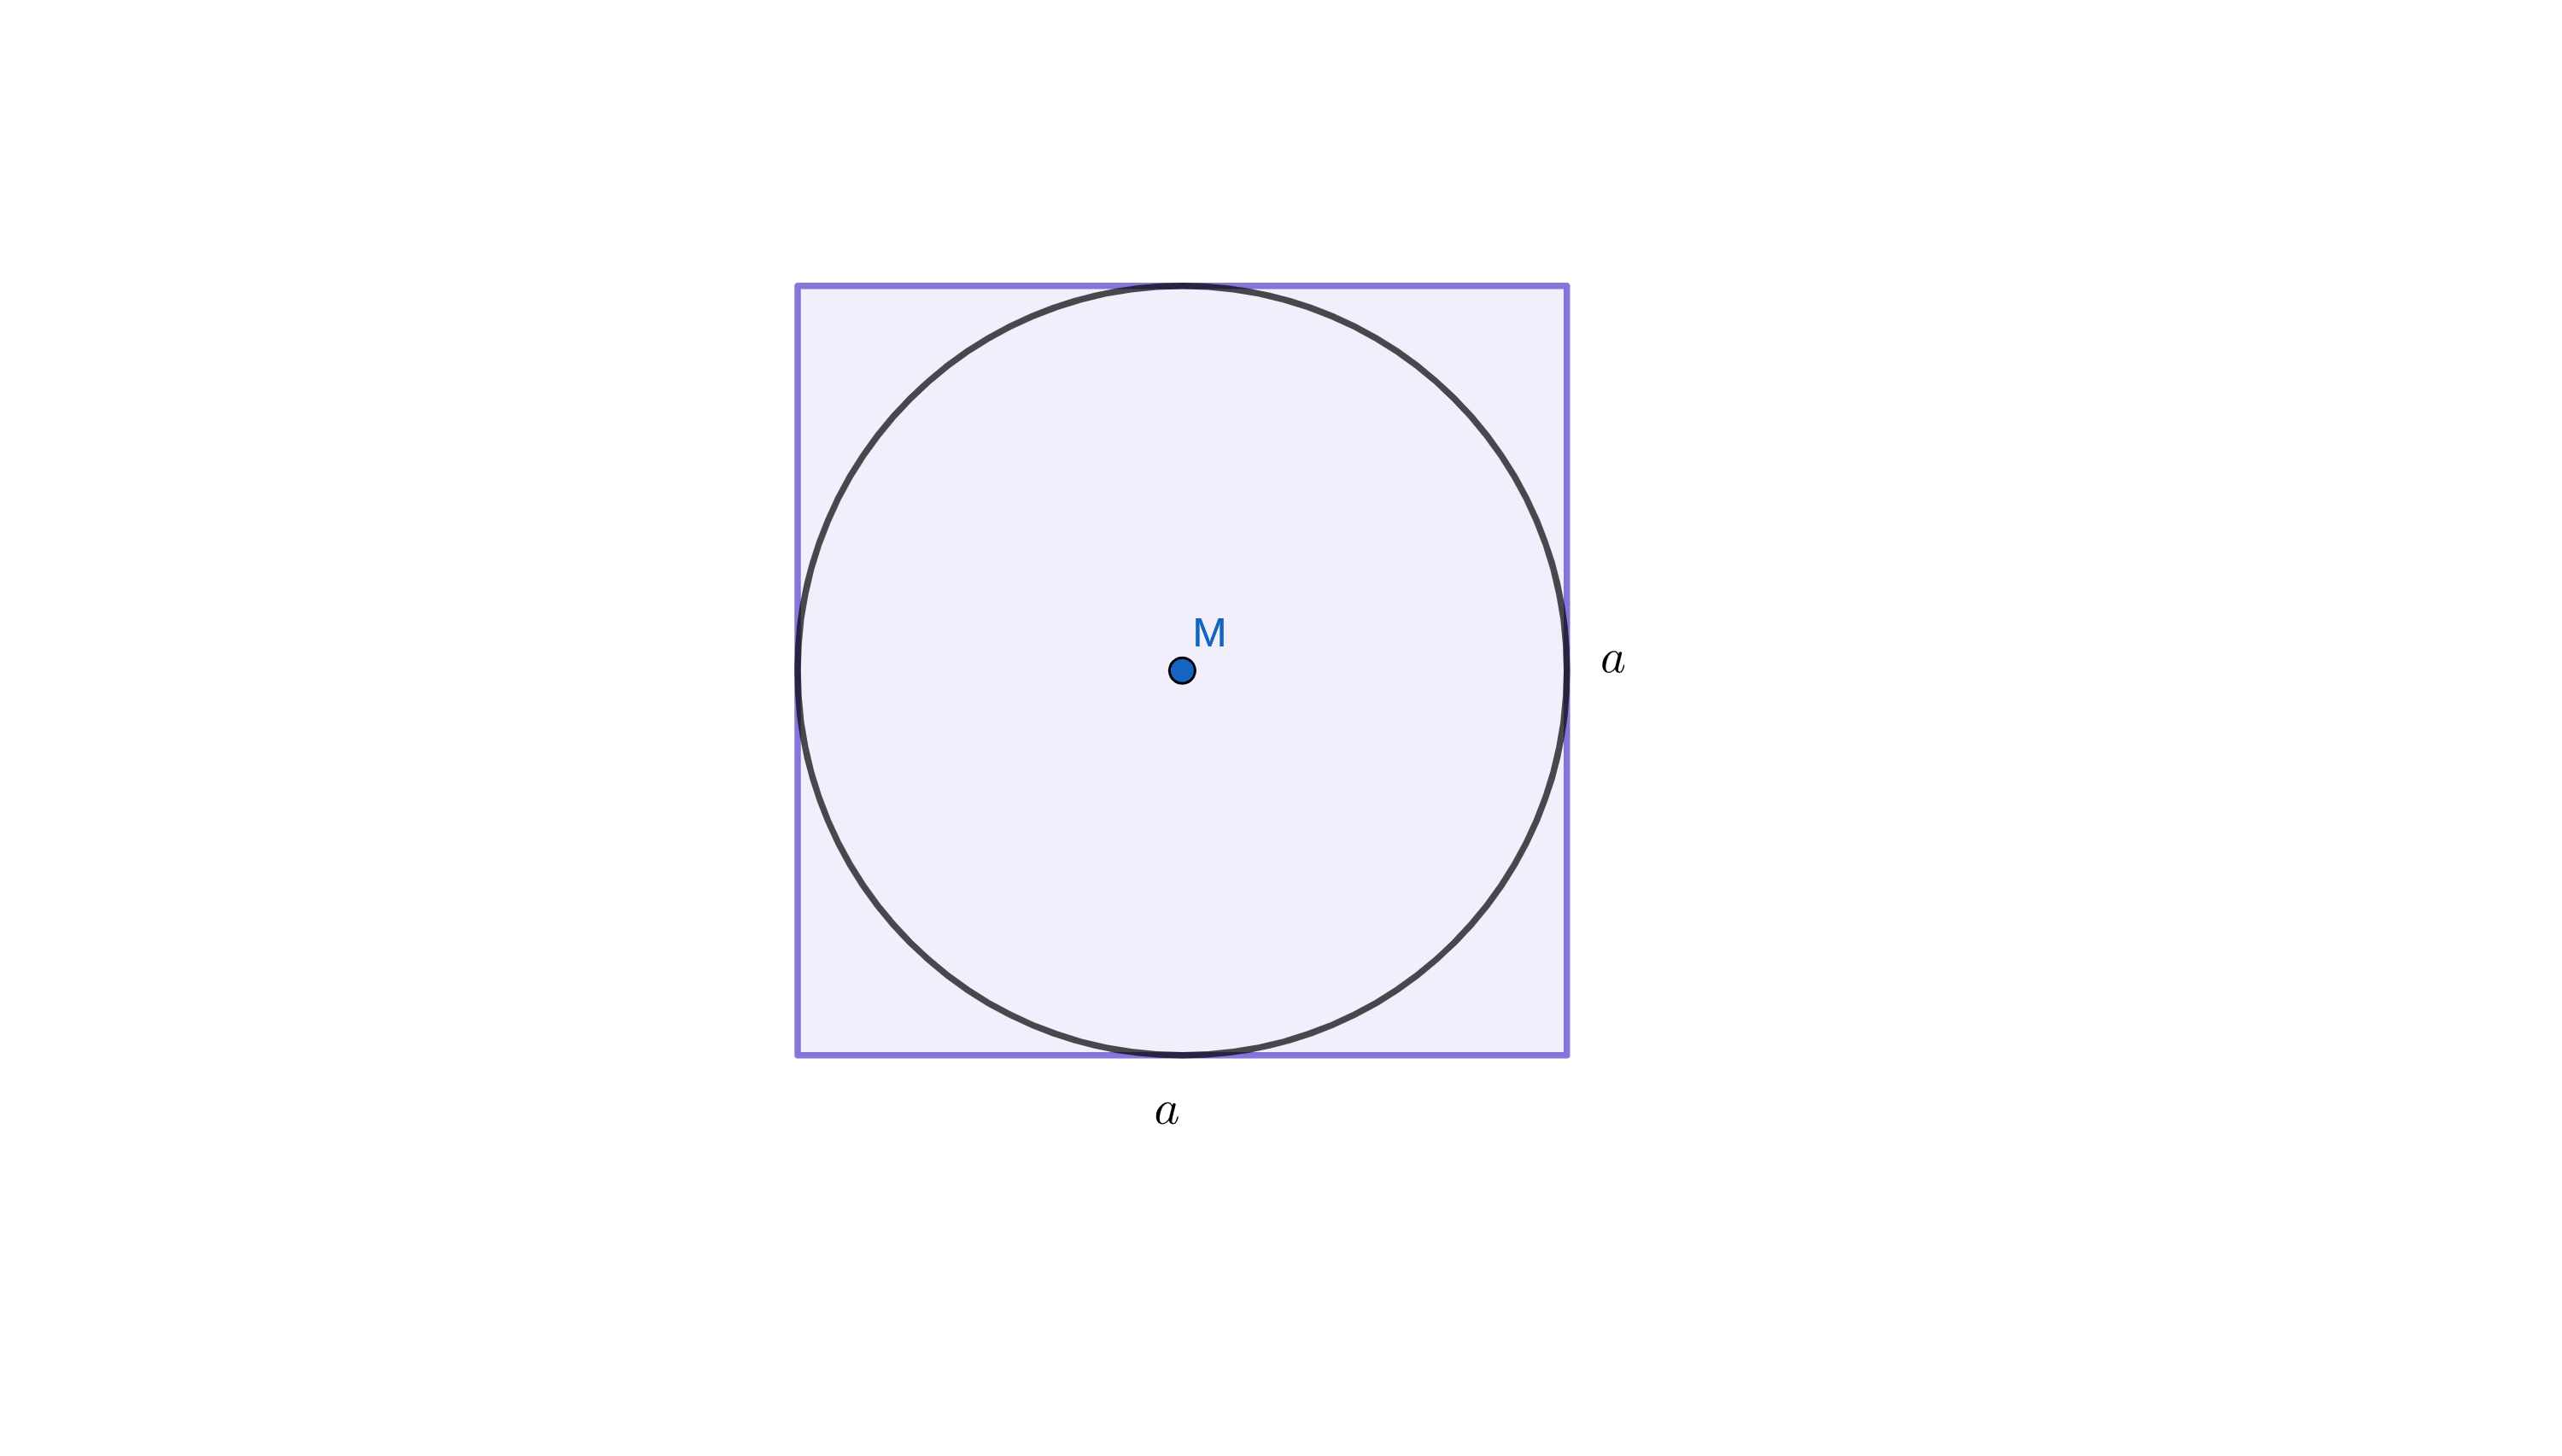
\includegraphics{./Bilder/KreisImQuadrat.png}

\begin{enumerate}
\def\labelenumi{\alph{enumi})}
\tightlist
\item
  Berechne den Verschnitt, wenn die Seite \(a\) 4m lang ist.
\end{enumerate}

Lösung

Ein Quadrat mit Seitenlänge \(4m\) hat den Flächeninhalt \(A_{Quadrat}=16m²\).

In diesem Fall hat der dem Quadrat einbeschriebene Kreis den Durchmesser \(d=4m\) und somit den Radius \(r=2m\).

Damit hat der Kreis einen Flächeninhalt von \(A_{Kreis}= \pi \cdot (2m)² = 4\pi\; m²\).

Der Verschnitt ergibt sich als Differenz der Quadratfläche und der Kreisfläche:

\[ \begin{align} Verschnitt &= A_{Quadrat} - A_{Kreis} =\\
{}\\
                            &= 16 \;m² - 4 \pi \;m² \\
                            {}\\
                            & \approx 3,43\; m^2\end{align}\]

\hypertarget{section-42}{%
\subsubsection*{}\label{section-42}}
\addcontentsline{toc}{subsubsection}{}

\begin{enumerate}
\def\labelenumi{\alph{enumi})}
\setcounter{enumi}{1}
\tightlist
\item
  Stelle eine Formel auf, mit der man den Flächeninhalt des Verschnitts in Abhängigkeit von \(a\) bestimmen kann.
\end{enumerate}

Lösung

\textbf{Vorüberlegung}

Der Verschnitt ergibt sich als Differenz der Quadratfläche und der Kreisfläche. Für die Quadratfläche gilt: \(A_{Quadrat}=a²\).

Der dem Quadrat einbeschriebene Kreis hat den Durchmesser \(d=a\) und damit den Radius \(r= {a \over 2}\). Für seine Fläche gilt also: \(A_{Kreis} = \pi \cdot ({a \over 2})^2\)

\textbf{Aufstellen der Formel}
\[ \begin{align} Verschnitt &= A_{Quadrat} - A_{Kreis} =\\
{}\\
                            &= a^2 - \pi \cdot ({a \over 2})^2 = \\
                            {}\\
                            & = a^2 - \pi \cdot {a^2 \over 4} = \\
                            {}\\
                            & = a^2 - {\pi \cdot a^2 \over 4} = \\
                            {}\\
                            & = a^2 - {\pi \over 4} \cdot a^2 =\\
                            {}\\
                            & = a^2 \cdot (1 - {\pi \over 4})
\end{align}\]

\hypertarget{section-43}{%
\subsubsection*{}\label{section-43}}
\addcontentsline{toc}{subsubsection}{}

\begin{enumerate}
\def\labelenumi{\alph{enumi})}
\setcounter{enumi}{2}
\tightlist
\item
  Wie viel Prozent der Gesamtfläche sind Verschnitt?
\end{enumerate}

Lösung

\textbf{Vorüberlegung}

Gefragt ist also, welchen Anteil der Verschnitt an der Gesamtfläche hat.

\textbf{Anteil des Verschnitts an der Gesamtfläche}

Man muss folgenden Quotienten berechnen:

\[ \begin{align} Anteil &= {Verschnitt \over Quadratfläche} = \\
{}\\
&= {a^2 \cdot (1 - {\pi \over 4}) \over a^2} = \\
{}\\
&= 1- {\pi \over4} \approx 0,2146
\end{align}\]

\textbf{Antwort}

Etwa 21,5\% der Fläche sind Verschnitt.

\hypertarget{section-44}{%
\subsubsection*{}\label{section-44}}
\addcontentsline{toc}{subsubsection}{}

\hypertarget{section-45}{%
\subsubsection*{}\label{section-45}}
\addcontentsline{toc}{subsubsection}{}

\hypertarget{section-46}{%
\subsubsection*{}\label{section-46}}
\addcontentsline{toc}{subsubsection}{}

\hypertarget{gemischte-aufgaben}{%
\subsection*{Gemischte Aufgaben}\label{gemischte-aufgaben}}
\addcontentsline{toc}{subsection}{Gemischte Aufgaben}

\hypertarget{aufgabe-1-7}{%
\subsubsection*{Aufgabe 1}\label{aufgabe-1-7}}
\addcontentsline{toc}{subsubsection}{Aufgabe 1}

Der Umfang eines Quadrates und eines Kreises beträgt jeweils 16 cm. Berechne und vergleiche die Flächeninhalte der beiden Figuren. Wie groß ist der Unterschied?

Lösung

\textbf{Gegeben}

\begin{itemize}
\tightlist
\item
  Ein Quadrat mit dem Umfang 16 cm.
\item
  Ein Kreis mit dem Umfang 16 cm.
\end{itemize}

\textbf{Flächeninhalt des Quadrates}

Ein Quadrat mit Umfang 16 cm hat eine Seitenlänge von \(16cm : 4 = 4cm\).

Daraus ergibt sich ein Flächeninhalt von \(A_{Quadrat} = 4cm \cdot 4cm = 16cm²\)

\textbf{Flächeninhalt des Kreises}

Für den Radius eines Kreises mit einem Umfang von 16 cm gilt: \(r = {U \over 2 \cdot \pi} = {16cm \over 2 \cdot \pi} \approx 2,55cm\).

Daraus ergibt sich ein Flächeninhalt von \(A_{Kreis}= \pi \cdot r^2 \approx \pi \cdot (2,55cm)^2 \approx 20,37 cm^2\)

\textbf{Vergleich der beiden Flächeninhalte}

Der Flächeninhalt des Kreises ist um \(A_{Kreis} - A_{Quadrat} \approx 20,37 cm² - 16 cm ² \approx 4,37 cm²\) größer als der Flächeninhalt des Quadrates.

\hypertarget{section-47}{%
\subsubsection*{}\label{section-47}}
\addcontentsline{toc}{subsubsection}{}

\hypertarget{aufgabe-2-7}{%
\subsubsection*{Aufgabe 2}\label{aufgabe-2-7}}
\addcontentsline{toc}{subsubsection}{Aufgabe 2}

Die größte Pizza der Welt wurde 2012 in Italien gebacken.

5 Pizzabäcker arbeiteten 48 Stunden lang an der Riesenpizza mit einem Durchmesser von 39,93m. Als Zutaten wurden 9900kg Mehl, 5000kg Tomatensoße, 4400kg Mozzarella und 125kg Parmesan verarbeitet.

\begin{enumerate}
\def\labelenumi{\alph{enumi})}
\tightlist
\item
  Welchen Flächeninhalt besaß diese Pizza?
\end{enumerate}

Lösung

Für den Radius der größten Pizza der Welt gilt:
\[r = {d \over 2} = {39,93\;m \over 2} = 19,965\; m\]

Für den Flächeninhalt der größten Pizza der Welt gilt:
\[ \begin{align} A &=\pi \cdot r^2 =\\
                   &= \pi \cdot (19,965\;m)² \approx \\
                   & \approx 1252,24\;m² \end{align}\]

\hypertarget{section-48}{%
\subsubsection*{}\label{section-48}}
\addcontentsline{toc}{subsubsection}{}

\begin{enumerate}
\def\labelenumi{\alph{enumi})}
\setcounter{enumi}{1}
\tightlist
\item
  Wie vielen Pizzen mit einem ``normalen'' Durchmesser von 30cm entspricht diese Fläche?
\end{enumerate}

Lösung

Für den Radius einer ``normalen'' Pizza gilt:
\[r = {d \over 2} = {0,3\;m \over 2} = 0,15\; m\]

Eine ``normale'' Pizza hat einen Flächeninhalt von
\[ \begin{align} A &= \pi \cdot (0,15\;m)^2 \approx \\
                    & \approx 0,070686\;m ^2 \end{align} \]

Wie viele ``normale'' Pizzen passen in die größte Pizza der Welt?

\[1252,24\;m² : 0,070686\;m ^2 \approx 17715,5\]

Die Fläche der größten Pizza der Welt entspricht etwa der 17715,5-fachen Fläche einer ``normalen'' Pizza.

\hypertarget{section-49}{%
\subsubsection*{}\label{section-49}}
\addcontentsline{toc}{subsubsection}{}

\begin{enumerate}
\def\labelenumi{\alph{enumi})}
\setcounter{enumi}{2}
\tightlist
\item
  Wie viele Männer wären notwendig gewesen, um diese Pizza auf einer Riesentafel zu umfassen? Rechne mit einer Spannweite von ungefähr 1,80m für jeden Mann.
\end{enumerate}

Lösung

Für den Umfang der größten Pizza der Welt gilt:
\[ \begin{align} U &= 2 \cdot \pi \cdot r =\\
                   &= 2 \cdot \pi \cdot 19,965\; m \approx \\
                   & \approx 125,44\;m \end{align}\]

Berechnung der Anzahl der Männer mit Spannweite \(1,80\;m\), die nötig sind, um die Riesenpizza zu umfassen:

\[125,44\;m : 1,80\;m \approx 70\]
70 Männer mit einer Spannweite von \(1,80\;m\) hätten die Weltrekordpizza umfassen können.

\hypertarget{section-50}{%
\subsubsection*{}\label{section-50}}
\addcontentsline{toc}{subsubsection}{}

\hypertarget{aufgabe-3-7}{%
\subsubsection*{Aufgabe 3}\label{aufgabe-3-7}}
\addcontentsline{toc}{subsubsection}{Aufgabe 3}

Eine hungrige Ziege wird mit einer ein Meter langen Schnur in der Mitte einer Wiese angepflockt. Damit sie die Wiese nach und nach abgrasen kann, wird die Schnur jeden Tag um einen Meter verlängert.

\begin{enumerate}
\def\labelenumi{\alph{enumi})}
\tightlist
\item
  Welche Formen haben die Flächen, die jeden Tag neu hinzukommen? Fertige eine Skizze an, berechne die Flächen für den 1., 2. und 3. Tag und trage deine Ergebnisse in eine Tabelle ein.
\end{enumerate}

\begin{longtable}[]{@{}lll@{}}
\toprule
& Länge des Seils (in Metern) & Neu hinzukommende Fläche (in m²)\tabularnewline
\midrule
\endhead
1. Tag & &\tabularnewline
2. Tag & &\tabularnewline
3. Tag & &\tabularnewline
4. Tag & &\tabularnewline
5. Tag & &\tabularnewline
6. Tag & &\tabularnewline
7. Tag & &\tabularnewline
8. Tag & &\tabularnewline
9. Tag & &\tabularnewline
10. Tag & &\tabularnewline
\bottomrule
\end{longtable}

Tipp

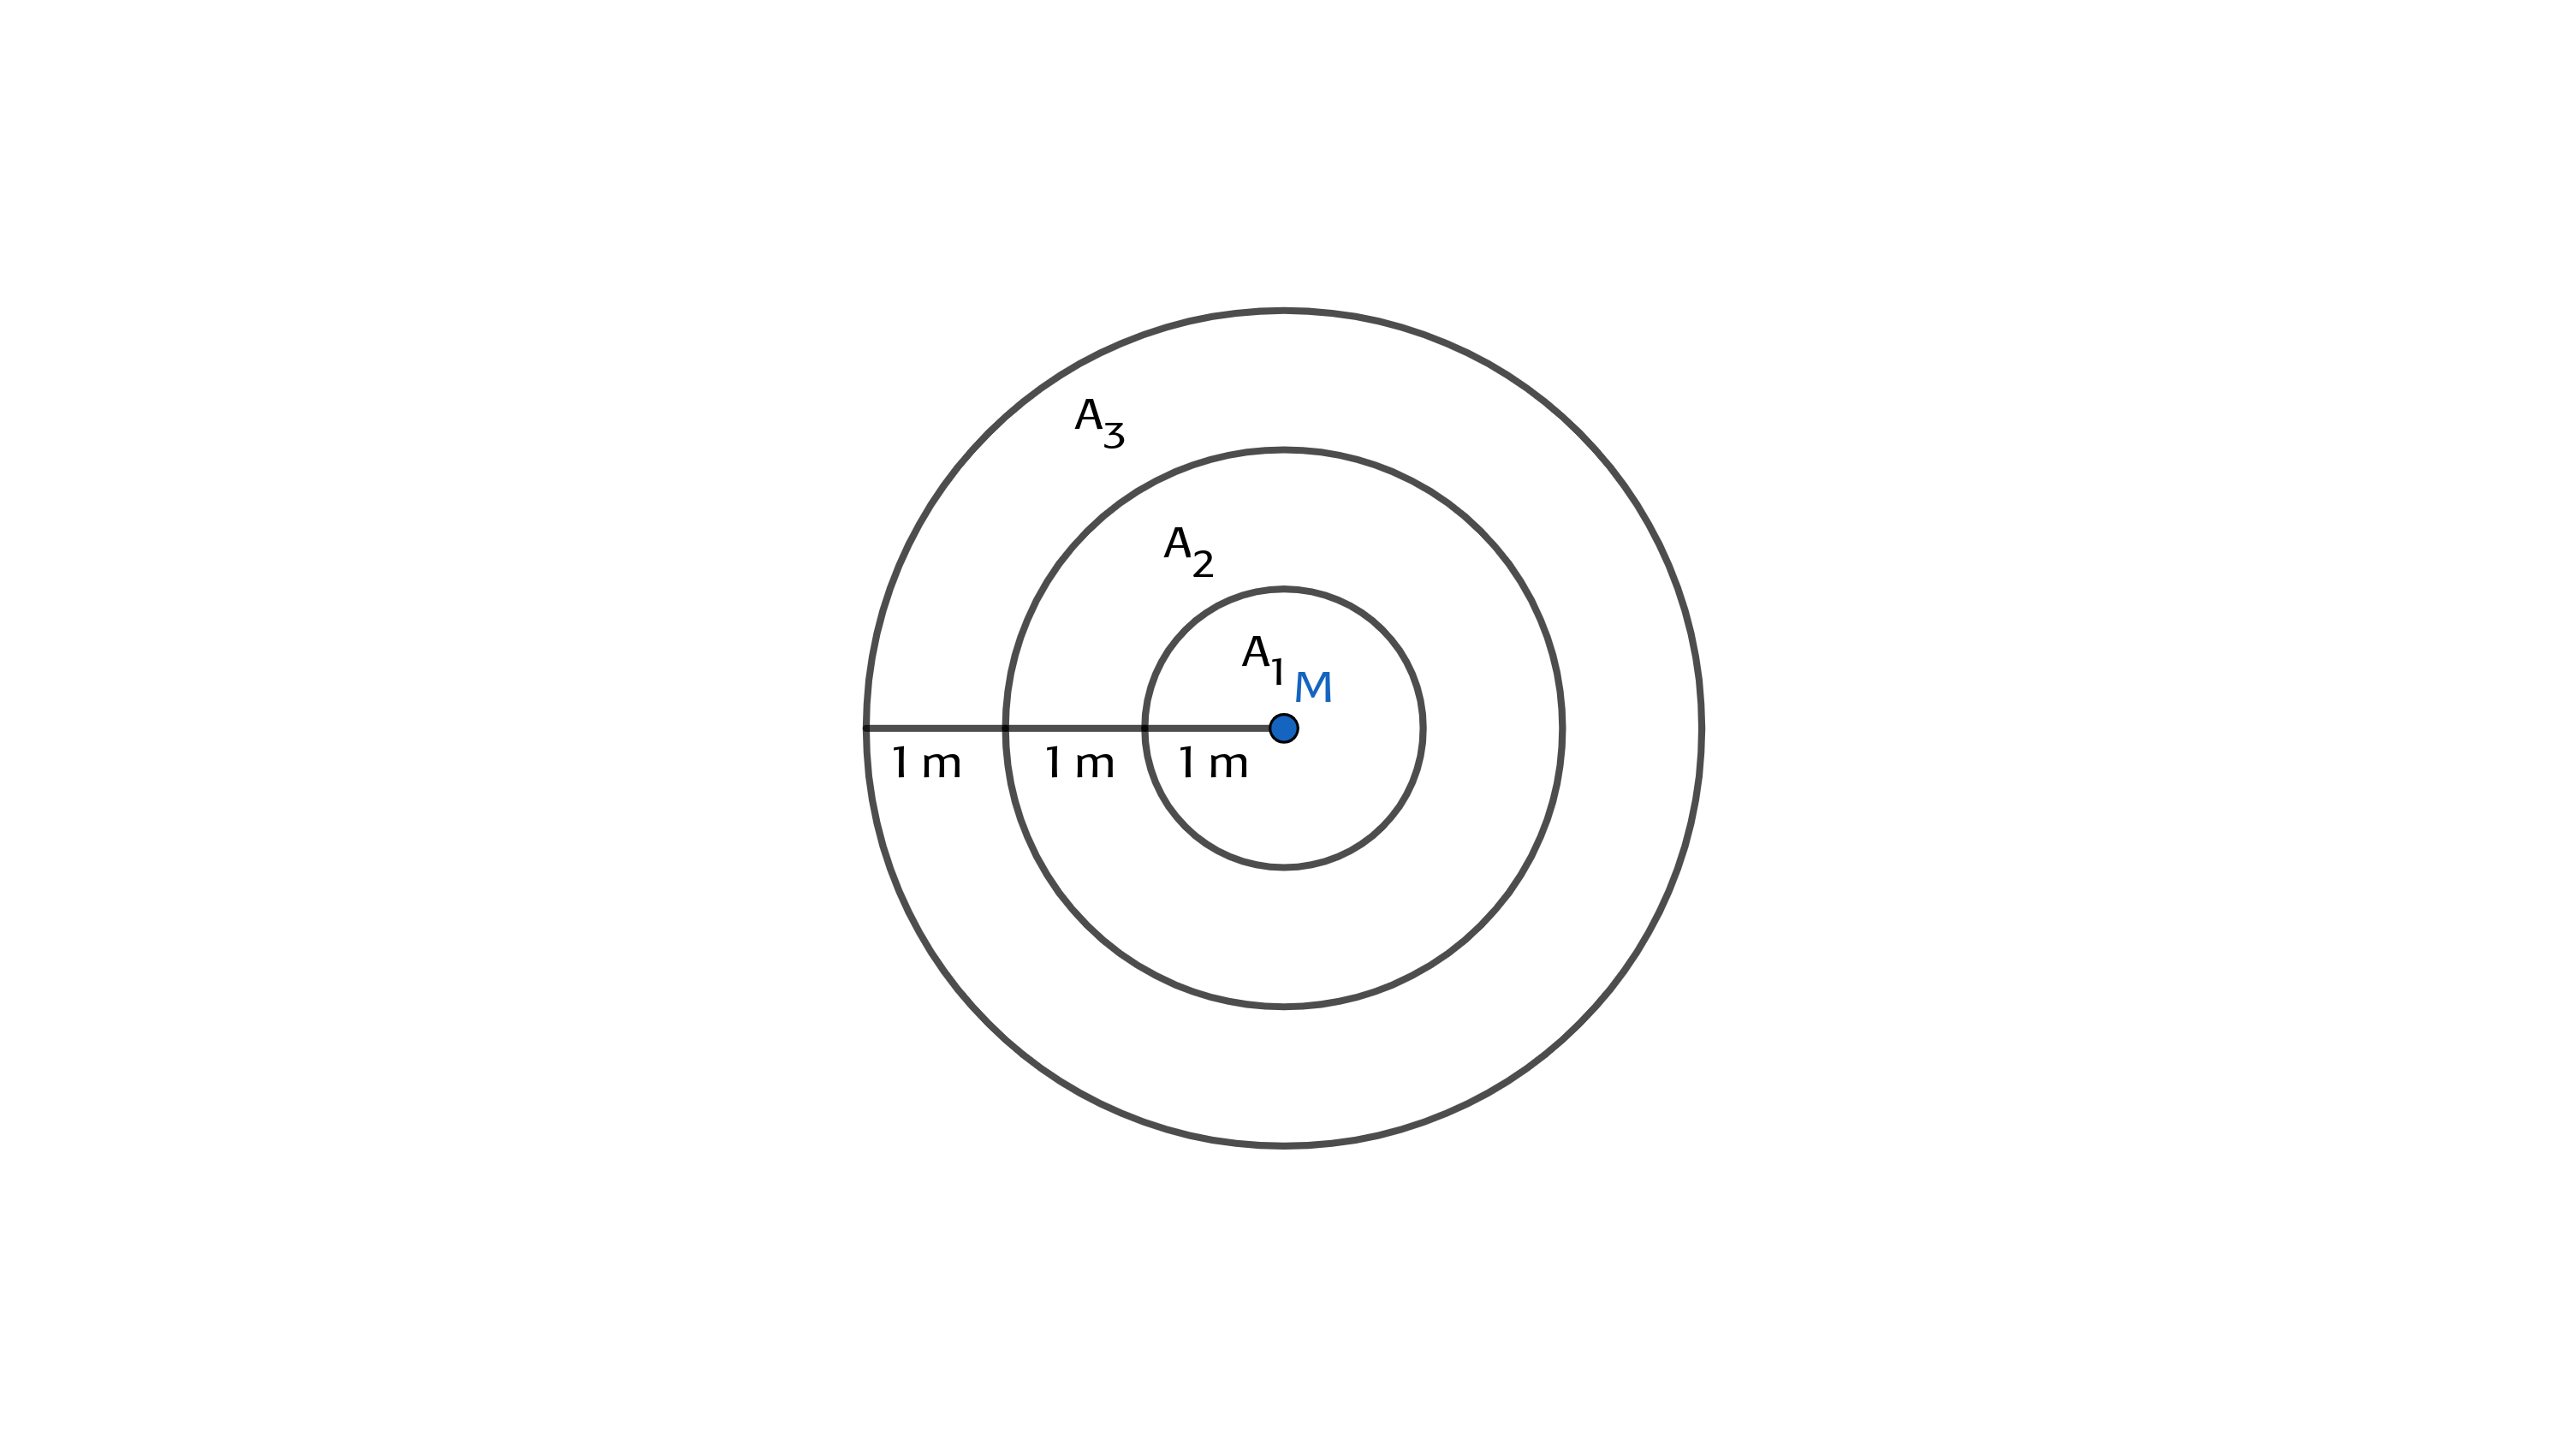
\includegraphics{./Bilder/hungrigeZiege.png}

\hypertarget{section-51}{%
\subsubsection*{}\label{section-51}}
\addcontentsline{toc}{subsubsection}{}

Lösung

Die erste Fläche \(A_1\) ist ein Kreis mit dem Radius \(1\;m\).

Alle weiteren Flächen sind Kreisringe mit der Breite \(1\;m\).

Die Skizze findest du im Tipp1 zur Teilaufgabe 1a).

\textbf{Berechnung der ersten drei Flächen}

\[\begin{align} A_1 & = \pi \cdot r^2_1 = \\
                    &= \pi \cdot (1m)^2 \approx 3,14\;m^2 \quad \end{align}\]

\[\begin{align} A_2 &= \pi \cdot r^2_2 - \pi \cdot r^2_1 =\\
                    &= \pi \cdot (2m)^2 - \pi\cdot 1\;m^2 =\\
                    &= \pi \cdot 4m^2 - \pi\;m^2 =\\
                    &= \pi \cdot (4m^2- 1m^2)=\\
                    &= 3\pi\;m^2\approx 9,42\;m^2
\end{align}\]

\[\begin{align} A_3 &= \pi \cdot r^2_3 - \pi \cdot r^2_2 =\\
                    &= \pi \cdot (3m)^2 - 4\pi\;m^2 =\\
                    &= \pi \cdot 9m^2 - 4\pi\;m^2 =\\
                    &= \pi \cdot (9m^2-4m^2)=\\
                    &= 5\pi\;m^2\approx 15,71\;m^2
\end{align}\]

Folglich sieht die Tabelle jetzt so aus:

\begin{longtable}[]{@{}lll@{}}
\toprule
& Länge des Seils (m) & Neu hinzu- kommende Fläche (m²)\tabularnewline
\midrule
\endhead
1. Tag & 1 & 3,14\tabularnewline
2. Tag & 2 & 9,42\tabularnewline
3. Tag & 3 & 15,71\tabularnewline
\bottomrule
\end{longtable}

\hypertarget{section-52}{%
\subsubsection*{}\label{section-52}}
\addcontentsline{toc}{subsubsection}{}

\begin{enumerate}
\def\labelenumi{\alph{enumi})}
\setcounter{enumi}{1}
\tightlist
\item
  Stelle nun eine allgemeine Berechnungsformel für die am n-ten Tag neu hinzukommende Fläche \(A(n)\) auf. Vervollständige mit Hilfe dieser Formel obige Tabelle.
\end{enumerate}

Tipp

Eine Formel zur Berechnung eines Kreisrings gab es schon mal\ldots{} In der Aufgabe mit dem Froschteich.

\hypertarget{section-53}{%
\subsubsection*{}\label{section-53}}
\addcontentsline{toc}{subsubsection}{}

Lösung

Das Seil, mit dem die Ziege angebunden ist, hat am n-ten Tag eine Länge von \(n\) Metern. Am Vortag, also am (n-1)-ten Tag, hatte das Seil eine Länge von \((n-1)\) Metern. Für die am n-ten Tag neu hinzukommende Fläche gilt somit:

\[\begin{align} A_n &= \pi \cdot r^2_n - \pi \cdot r^2_{n-1}=\\
                    &=\pi \cdot n^2 - \pi \cdot (n-1)^2=\\
                    &= \pi \cdot n^2 - \pi \cdot (n^2 - 2n + 1)= \\
                    &=\pi \cdot (n^2 - (n^2- 2n + 1))=\\
                    &=\pi \cdot (n^2- n^2+2n-1)=\\
                    &=\pi \cdot(2n-1)
\end{align}\]

Damit ergibt sich folgende Tabelle:

\begin{longtable}[]{@{}lll@{}}
\toprule
& Länge des Seils (m) & Neu hinzu- kommende Fläche (m²)\tabularnewline
\midrule
\endhead
1. Tag & 1 & 3,14\tabularnewline
2. Tag & 2 & 9,42\tabularnewline
3. Tag & 3 & 15,71\tabularnewline
4. Tag & 4 & 21,99\tabularnewline
5. Tag & 5 & 28,27\tabularnewline
6. Tag & 6 & 34,56\tabularnewline
7. Tag & 7 & 40,84\tabularnewline
8. Tag & 8 & 47,12\tabularnewline
9. Tag & 9 & 53,41\tabularnewline
10. Tag & 10 & 59,69\tabularnewline
\bottomrule
\end{longtable}

\hypertarget{section-54}{%
\subsubsection*{}\label{section-54}}
\addcontentsline{toc}{subsubsection}{}

\begin{enumerate}
\def\labelenumi{\alph{enumi})}
\setcounter{enumi}{2}
\tightlist
\item
  Welche Fläche hat die Ziege nach 15 Tagen insgesamt abgegrast?
\end{enumerate}

Lösung

Nach 15 Tagen hat die Ziege eine Kreisfläche mit einem Radius von \(15\) Metern abgefressen. Also:

\[\begin{align} F_{abgegrast} &= \pi \cdot (15m)^2=\\
                              &= 225\pi\;m^2 \approx \\
                              &\approx 706,86\;m^2\end{align}\]

\hypertarget{section-55}{%
\subsubsection*{}\label{section-55}}
\addcontentsline{toc}{subsubsection}{}

\begin{enumerate}
\def\labelenumi{\alph{enumi})}
\setcounter{enumi}{3}
\tightlist
\item
  Wie viele Tage müssen mindestens vergehen, damit die Ziege insgesamt mehr als 150m² abgegrast hat?
\end{enumerate}

Lösung

\textbf{Vorüberlegung}
Gefragt ist, wann die abgefressene Kreisfläche größer oder gleich 150m² ist. Der Radius des Kreises entspricht dabei der Seillänge, aus der praktischer Weise ganz einfach auf die Anzahl der vergangenen Tage geschlossen werden kann. Das Seil hat ja am ersten Tag eine Länge von einem Meter, am zweiten Tag eine Länge von zwei Metern, am dritten Tag eine Länge von drei Metern usw. Am n-ten Tag hat es eine Länge von n Metern.

Wenn man also den Radius des Kreises kennt, weiß man, wann die Ziege 150m² ``gemäht'' hat.

\textbf{Berechnung der zu 150m² passenden Seillänge l}

\[\begin{align} l &= \sqrt{A\over\pi}\\
                  & = \sqrt{150\;m^2 \over \pi} \approx\\
                  &\approx 7\;m\end{align}\]

Wenn das Seil \(7\;m\) lang ist, hat die Ziege 150m² abgefressen. Es braucht also 7 Tage.

\textbf{Alternative:}

Addiere die in der Tabelle festgehaltenen Werte für die neu hinzugekommene Fläche, bis der Wert 150 übersteigt. Also:
\(3,14 + 9,42 + 15,71 + 21,99 + ...\overset{?}{=}150\)

\hypertarget{section-56}{%
\subsubsection*{}\label{section-56}}
\addcontentsline{toc}{subsubsection}{}

\hypertarget{aufgabe-4-6}{%
\subsubsection*{Aufgabe 4}\label{aufgabe-4-6}}
\addcontentsline{toc}{subsubsection}{Aufgabe 4}

Es ist ein heißer Sommer. Etwas Abkühlung ist gefragt. Auch Anna, die gerade 12 Jahre alt geworden ist, jammert über die Hitze. Da bringt ihre Oma aus dem Baumarkt ein rundes Planschbecken mit. Laut Verpackung benötigt es in aufgebautem Zustand \(2\;m^2\) Fläche. Anna schimpft:" Das ist ja viel zu klein für mich!" Hat sie Recht?

Lösung

\textbf{Vorüberlegung}

Gesucht ist der Durchmesser des Planschbeckens. Kennt man ihn, kann man vielleicht abschätzen, ob sich Anna noch bequem in das Planschbecken legen kann.

\textbf{Ermittlung des Durchmessers}

Gegeben ist die Kreisfläche: \(A = 2\;m^2\)

Folglich gilt für den Radius: \(r = \sqrt{A \over \pi} \approx 0,8\;m\)

Damit ergibt sich ein Durchmesser von etwa \(1,60\;m\)

\textbf{Antwort}

Da Mädchen mit 12 Jahren im Durchschnitt \(1,49\;m\) sind, kann man davon ausgehen, dass Anna zumindest bequem im Wasser liegen kann. Mit Schwimmen wird's aber nix.

\hypertarget{section-57}{%
\subsubsection*{}\label{section-57}}
\addcontentsline{toc}{subsubsection}{}

\hypertarget{aufgabe-5-2}{%
\subsubsection*{Aufgabe 5}\label{aufgabe-5-2}}
\addcontentsline{toc}{subsubsection}{Aufgabe 5}

Beim Torwandschießen versucht man, einen Fußball durch ein Loch zu schießen. Die Löcher haben dabei einen Durchmesser von \(55\;cm\). Ein Fußball hat einen Umfang von maximal \(70\;cm\). Wie viel Platz ist zwischen dem Ball und dem Rand des Loches, wenn man genau mittig trifft?

Lösung

\textbf{Berechnung des Fußballdurchmessers}

Es gilt: \(d={U \over \pi} \approx 22,3\;cm\)

\textbf{Vergleich der beiden Durchmesser}

Der Durchmesser des Torwandloches ist um ungefähr \(55\;cm - 22,3\;cm \approx 32,7\;cm\) größer als der Durchmesser des Balles.

\textbf{Platz zwischen dem Ball und dem Rand des Loches}

Da auf beiden Seiten gleich viel Abstand zum Rand des Torwandloches sein soll, muss man diese Differenz noch halbieren.

Also sind rund um den Ball noch etwa \(32,7\;cm : 2 \approx 16,35\;cm\) Platz.

\hypertarget{section-58}{%
\subsubsection*{}\label{section-58}}
\addcontentsline{toc}{subsubsection}{}

\hypertarget{aufgabe-6-1}{%
\subsubsection*{Aufgabe 6}\label{aufgabe-6-1}}
\addcontentsline{toc}{subsubsection}{Aufgabe 6}

Es ist Corona. Trotzdem - zumindest die Abiturprüfungen können wohl nicht vom heimischen Rechner aus geschrieben werden. Nun stellt sich die Frage, wieviele Abiturienten gleichzeitig in der Aula ihre Abiturprüfung schreiben dürfen\ldots.

Nimm an, die Aula sei quadratförmig und habe einen Flächeninhalt von \(100\;m^2\). Die Abiturienten müssen natürlich einen Abstand von 2m zueinander einhalten.

\begin{enumerate}
\def\labelenumi{\alph{enumi})}
\item
  Wie viele Abiturienten passen unter diesen Bedingungen in die Aula? Erstelle zunächst eine Skizze!
\item
  Die drei Mathelehrer, die mit der Bearbeitung dieser Aufgabe betraut wurden, kommen leider zu recht unterschiedlichen Ergebnissen und geraten darüber in Streit. Herr A. behauptet fest, es würden lediglich 25 Abiturient:innen in die Aula passen. Herr B. dagegen, berechnet die für jede:n benötigte Kreisfläche und folgert, dass 31 Abiturient:innen in die Aula passen. Bei Herrn C., der die punktförmigen Abiturient:innen auch an die Wand setzt, passen sogar 36 Personen in die Aula. Vollziehe die drei Ansätze nach! Erstelle zu jeder Situation entweder eine Skizze oder führe eine kurze Rechnung durch.
\item
  Wie kann es sein, dass Herr C. 36 Abiturient:innen in die Aula stecken kann, obwohl Herr B. doch durch Rechnung gezeigt hat, dass nur 31 Personen unter Coronabedingungen in die Aula passen?
\item
  Herr B., der niemandem mehr als die minimal benötigte Kreisfläche zugestehen möchte, ist erbost über die Flächenverschwendung von Herrn A. Wie viel Prozent der Fläche ``verschwendet'' Herr A.? Wie viel Prozent der Fläche ``verschwendet'' Herr C., von dessen Ansatz Herr B. begeistert ist?
\end{enumerate}

Lösung

\hypertarget{section-59}{%
\subsubsection*{}\label{section-59}}
\addcontentsline{toc}{subsubsection}{}

\hypertarget{trainingsraum}{%
\chapter{Trainingsraum}\label{trainingsraum}}

Du hast jetzt alle Formeln und Flächen kennengelernt und auch bereits viele Aufgaben gerechnet. Hier gibt es noch eine Übersicht über alle Formeln und ein paar letzte Aufgaben, zum Üben und Einprägen des Erarbeiteten.

Viel Spaß und Erfolg!

\hypertarget{uxfcbersicht-uxfcber-alle-vorgekommenen-formeln}{%
\section*{Übersicht über alle vorgekommenen Formeln}\label{uxfcbersicht-uxfcber-alle-vorgekommenen-formeln}}
\addcontentsline{toc}{section}{Übersicht über alle vorgekommenen Formeln}

\hypertarget{formeln-zuordnen}{%
\section*{Formeln zuordnen}\label{formeln-zuordnen}}
\addcontentsline{toc}{section}{Formeln zuordnen}

\hypertarget{dropZone}{}
\hypertarget{dropBox1}{}
Trapezfläche

\hypertarget{dropBox2}{}
\(A=\pi \cdot r^2\)

\hypertarget{dropBox3}{}
\(\sqrt{7}\)

\hypertarget{dropBox4}{}
Hund

\hypertarget{animals}{}
Hier der Text

\hypertarget{trainingsaufgaben}{%
\section*{Trainingsaufgaben}\label{trainingsaufgaben}}
\addcontentsline{toc}{section}{Trainingsaufgaben}

\hypertarget{das-kannst-du-jetzt}{%
\chapter{Das kannst du jetzt\ldots{}}\label{das-kannst-du-jetzt}}

Wie immer im Matheunterricht werden dir die Inhalte dieses Themas wiederbegegnen. Daher findest du hier zunächst eine Checkliste, die dir als Orientierung dienen soll, ob du die besprochenen Themen verinnerlicht hast. Lies sie dir bitte gründlich durch. Solltest du nicht wissen, was mit dem jeweiligen Punkt gemeint ist, oder ahnen, dass du in einem Bereich Lücken hast, bearbeite bitte zunächst die in der letzten Spalte verlinkten Materialien - einfach auf ``nachlesen'' klicken.

Wenn du der Ansicht bist, dass du eigentlich alles (wieder) weißt, geht es mit dem \textbf{Abschlussquiz} weiter. Bearbeite das Quiz und arbeite immer dann, wenn du eine Aufgabe nicht lösen konntest oder sie falsch gelöst hast, die zu diesem Thema auf der Checkliste verlinkten Materialien zum ``Nachlesen'' durch.

\hypertarget{checkliste}{%
\section{Checkliste}\label{checkliste}}

\begin{table}[H]
\centering
\begin{tabular}[t]{l|l|l}
\hline
Themenbereich & Ich kann & Was war das doch gleich?\\
\hline
Umgang mit Termen & ... Terme mit mehreren Variablen aufstellen & [Terme aufstellen](https://gdischinger.github.io/Mathe\_8d/03FormelnErstellen/Grundlagen/TermeAufstellen.html)\\
\hline
 &  & \\
\hline
 & ... gleichartige Terme zusammenfassen & [Umgang mit Termen](https://gdischinger.github.io/Mathe\_8d/03FormelnErstellen/Grundlagen/TermeZusammenfassen.html)\\
\hline
 & ... Plus- und Minusklammern in Termen auflösen & \\
\hline
 & ... Terme mit Zahlen multiplizieren und durch Zahlen dividieren & \\
\hline
 & ... Terme mit Hilfe der Vorrangregeln vereinfachen & \\
\hline
 & ... eine Klammer in Termen ausmultiplizieren & \\
\hline
 & ... gemeinsame Faktoren aus Summen oder Differenzen ausklammern & \\
\hline
 & ... zwei Klammern in Termen ausmultiplizieren & \\
\hline
 & ... die binomischen Formeln anwenden. & [Binomische Formeln](https://gdischinger.github.io/Mathe\_8a/03FormelnErstellen/Grundlagen/BinomischeFormeln.html)\\
\hline
 &  & \\
\hline
Dreieck & ... den Flächeninhaltes eines Dreiecks berechnen & [Dreieck](https://gdischinger.github.io/Mathe\_8d/03FormelnErstellen/Dreieck.html)\\
\hline
 & ... die Grundseite eines Dreiecks berechnen, wenn der Flächeninhalt und die Höhe gegeben sind. & \\
\hline
 & ... die Höhe eines Dreiecks berechnen, wenn der Flächeninhalt und die Grundseite gegeben sind. & \\
\hline
 &  & \\
\hline
Trapez & ... den Flächeninhalt eines Trapezes berechnen. & [Trapez](https://gdischinger.github.io/Mathe\_8d/03FormelnErstellen/Trapez.html)\\
\hline
 & ... die Höhe eines Trapezes berechnen, wenn der Flächeninhalt und die Längen der beiden parallelen Seiten gegeben sind. & \\
\hline
 & ... die Länge einer der parallelen Seiten eines Trapezes berechnen, wenn der Flächeninhalt und die Höhe gegeben sind. & \\
\hline
 &  & \\
\hline
Parallelogramm & ... den Flächeninhalt eines Parallelogramms berechnen. & [Parallelogramm](https://gdischinger.github.io/Mathe\_8d/03FormelnErstellen/Parallelogramm.html)\\
\hline
 & ... die Grundseite eines Parallelogramms berechnen, wenn der Flächeninhalt und die Höhe gegeben sind. & \\
\hline
 & ... die Höhe eines Parallelogramms berechnen, wenn der Flächeninhalt und die Grundseite gegeben sind. & \\
\hline
 &  & \\
\hline
Vieleck & Flächeninhalte zusammengesetzter Figuren berechnen & [Vieleck](https://gdischinger.github.io/Mathe\_8d/03FormelnErstellen/Vieleck.html)\\
\hline
 &  & \\
\hline
Kreis & ... den Flächeninhalt eines Kreises berechnen. & [Kreis](https://gdischinger.github.io/Mathe\_8d/03FormelnErstellen/Kreis.html)\\
\hline
 & ... den Umfang eines Kreises berechnen. & \\
\hline
 & .. den Radius/Durchmesser eines Kreises berechnen, wenn der Flächeninhalt des Kreises gegeben ist. & \\
\hline
 & ... den Radius/Durchmesser eines Kreises berechnen, wenn der Umfang des Kreises gegeben ist. & \\
\hline
 & ... den Radius eines Kreises berechnen, wenn der Durchmesser des Kreises gegeben ist und umgekehrt. & \\
\hline
\end{tabular}
\end{table}

\hypertarget{abschlussquiz}{%
\section{Abschlussquiz}\label{abschlussquiz}}

Bearbeite folgende Aufgaben. Du brauchst dazu \textbf{einen Zettel und einen Stift}! Beachte bitte, dass auch \textbf{mehrere Lösungen richtig} sein können. Überprüfe am Ende deine Ergebnisse und \textbf{stelle deine Rechnungen in OneNote ein} - im Abschnitt Hausaufgaben auf einer Seite mit dem Titel 24. Februar. Manche Aufgaben kannst du vielleicht ohne Zwischenschritte lösen, dann müssen sie auch nicht auf deinem Schmierpapier vermerkt sein. Andere Aufgaben wirst du aber nicht ohne Zwischenschritte lösen können\ldots.

  \bibliography{book.bib,packages.bib}

\end{document}
